\documentclass[a4paper]{article}
\usepackage{spconf}

% \usepackage[utf8]{inputenc}

% \usepackage{graphicx, url}
% \usepackage{amsmath, amsfonts, xfrac}
% \usepackage{mathtools}

\usepackage{multirow}

\usepackage[utf8]{inputenc}

\usepackage[mathcal]{euscript}
\usepackage{booktabs}

\usepackage{graphicx, url}

\usepackage[cmex10]{amsmath}
\usepackage{amsmath, amsfonts, amssymb, amsthm}
\usepackage{mathptmx}

\usepackage{subcaption}
\usepackage{float}

\usepackage[nocompress]{cite}


\usepackage{tikz}
\usetikzlibrary{positioning}

\newcommand{\Real}{\mathbb{R}}
\newcommand{\Cplx}{\mathbb{C}}

\newcommand{\pr}{\mathbb{P}}
\newcommand{\ex}{\mathbb{E}}
\newcommand{\var}{\text{var}}
\newcommand{\Pcal}{\mathcal{P}}
\newcommand{\Dcal}{\mathcal{D}}
\newcommand{\Ncal}{\mathcal{N}}
\newcommand{\Lcal}{\mathcal{L}}

\newcommand{\defn}{\mathop{\overset{\Delta}{=}}\nolimits}
\newcommand{\lpto}{\mathop{\overset{L^p}{\to}}\nolimits}

\newcommand{\re}{\operatorname{Re}\nolimits}
\newcommand{\im}{\operatorname{Im}\nolimits}

\title{Numerical study of the Crossing Tree for Self-similar Processes}
\twoauthors
  {Ivan Nazarov}
    {IITP RAS, Skoltech\\ Moscow, Russia}
  {Geoffrey Decrouez}
    {National Research University\\ Higher School of Economics\\ Moscow, Russia}

\begin{document}
\maketitle

\begin{abstract}
The crossing tree is a method for studying multi-resolution properties of time series,
in particular scale invariance. It provides an ad-hoc representation of the signal
independent of the time scale across a wide range of resolutions and. In this paper
we conduct a numerical study of the statistical properties of the structure of the
crossing tree for typical monofractal scale-invariant processes. We gather evidence
supporting shared common features of across crossing trees of the processes of this
class.
\end{abstract}


 a recent tool, created to study scale invariance properties
exhibited by network traffic, financial time-series, and natural phenomena in physics
and biology, such as turbulence, earthquakes and heart beat.

\section{Introduction} % (fold)
\label{sec:introduction}

A process is self-similar (or scale-invariant) if its trajectories share similar
characteristic dynamic patterns across multiple time-scales. Time series with this
phenomenon have been observed in EEG and ECG traces, seismology, hydrodynamics,
network traffic and high frequency finance, \cite{}.
% references
A typical approach to studying self-similar is to use wavelet-based coefficients
to analyze and correlate dynamic patterns across different time resolutions of a
process, \cite{Jaffard2007}. Wavelet-based multi-resolution analysis requires specifying
a reference pattern, i.e. the mother wavelet, and favours regularly samples time
series. An alternative approach is to use a crossing tree -- a concept introduced
in \cite{BarlowPerkins88} to study diffusion on fractal sets. In \cite{jones2004}
it was used to study self-similarity and local regularity in network traffic data.
The crossing tree is a path adapted method which relies on a space decomposition
of the signal and as such can be applied to irregular time series, \cite{decrouez2013}.
In \cite{decrouez2015} it was shown that the estimates of the singularity spectrum
under the multifractal formalism provided by the crossing tree approach have better
properties compared to the wavelet-based methods.

In this paper we conduct a small numerical experiment to find evidence for common
statistical properties of the crossing tree shared across different type of self-similar
monofractal processes. First, based on the results in \cite{ECP1673}, we make a
conjecture on the distribution of the structure of the tree, and the average duration
of crossings. The paper is structured as follows: the construction of a crossing tree
is given in sec.~\ref{sec:the_crossing_tree}, in sec.~\ref{sec:self_sim_processes}
we review the self-similar processes used in the study, and sec.~\ref{sec:experiment}
outlines the setup and discusses the results of the Monte Carlo experiment.

% section introduction (end)

\section{The crossing tree} % (fold)
\label{sec:the_crossing_tree}

In this section we construct a crossing tree of a real-valued process $(X(t))_{t\in[0, \infty)}$
with almost surely continuous paths. The tree reveals scale invariance through hitting
times of within lattices with increasingly coarser spatial resolution. If $\delta>0$
is the resolution of the base lattice, then the crossing tree naturally arises from
the succession of hitting times of adjacent uniformly spaced lattices $(x_0 + \delta 2^n \mathbb{Z})_{n\geq 0}$
with a fixed origin $x_0\in \Real$.

The crossing times $(T_k^n)_{k\geq0}$ of the $\delta 2^n \mathbb{Z}$ lattice, the
\emph{$n$-th level crossing times}, are defined iteratively: for any $k\geq 0$
\begin{equation} \label{eq:xing_time}
  T_{k+1}^n = \inf\bigl\{t\geq T_k^n\,:\,
        X(t)\in x_0 + \delta 2^n \mathbb{Z}\,, X(t)\neq X(T^n_k)
    \bigr\} \,,
\end{equation}
with $T_0^n = 0$. Though in general $T_0^n$ is not a crossing time, without the
loss of generality of the construction, we can consider processes starting at the
origin $X(0)=x_0=0$. In this case for continuous processes this definition is equivalent
to the first hitting time $t\geq T_k^n$ with $|X(t) - X(T^n_k)| \geq \delta 2^n$.
Thus we define the \emph{$n$-th level crossing} as the slice of the process over
$[T_k^n, T_{k+1}^n)$, $k\geq 0$, during which it moves at least $\pm \delta 2^n$.
The duration of the $k$-th $n$-the level crossing, $n\geq0$, is $W_{k+1}^n = T_{k+1}^n - T_k^n$.

The crossing tree naturally emerges from the alignment between the crossings of
lattices with adjacent resolutions $\delta 2^n \mathbb{Z}$ and $\delta 2^{n+1} \mathbb{Z}$.
A typical crossing tree along with a process, over which it was constructed is depicted
in fig.~\ref{fig:sample_tree}. In \cite{decrouez2013,ECP1673} the tree is constructed
over resolutions $\delta 2^n \mathbb{Z}$ even for negative $n$. Though, in practice
the time series are sampled at finite frequency and it is unreasonable to go beyond
the finest lattice $\delta \mathbb{Z}$, in theory infinitely fine and coarse resolutions
give a one-to-one description of the underlying continuous random process in terms
of the scale $\delta$, the crossing times $(T_k^n)_{k\geq 0}$, and the crossing
orientations $(\alpha_k^n)_{k\geq 1}$ given by
\begin{equation*} \label{eq:xing_orientations}
    \alpha_k^n = \text{sign}\bigl( X(T_k^n) - X(T_{k-1}^n) \bigr) \,.
\end{equation*}
% In the following we establish the emergent tree-structure.

\begin{figure}[ht]
    \centering
    \begin{subfigure}{\linewidth}
        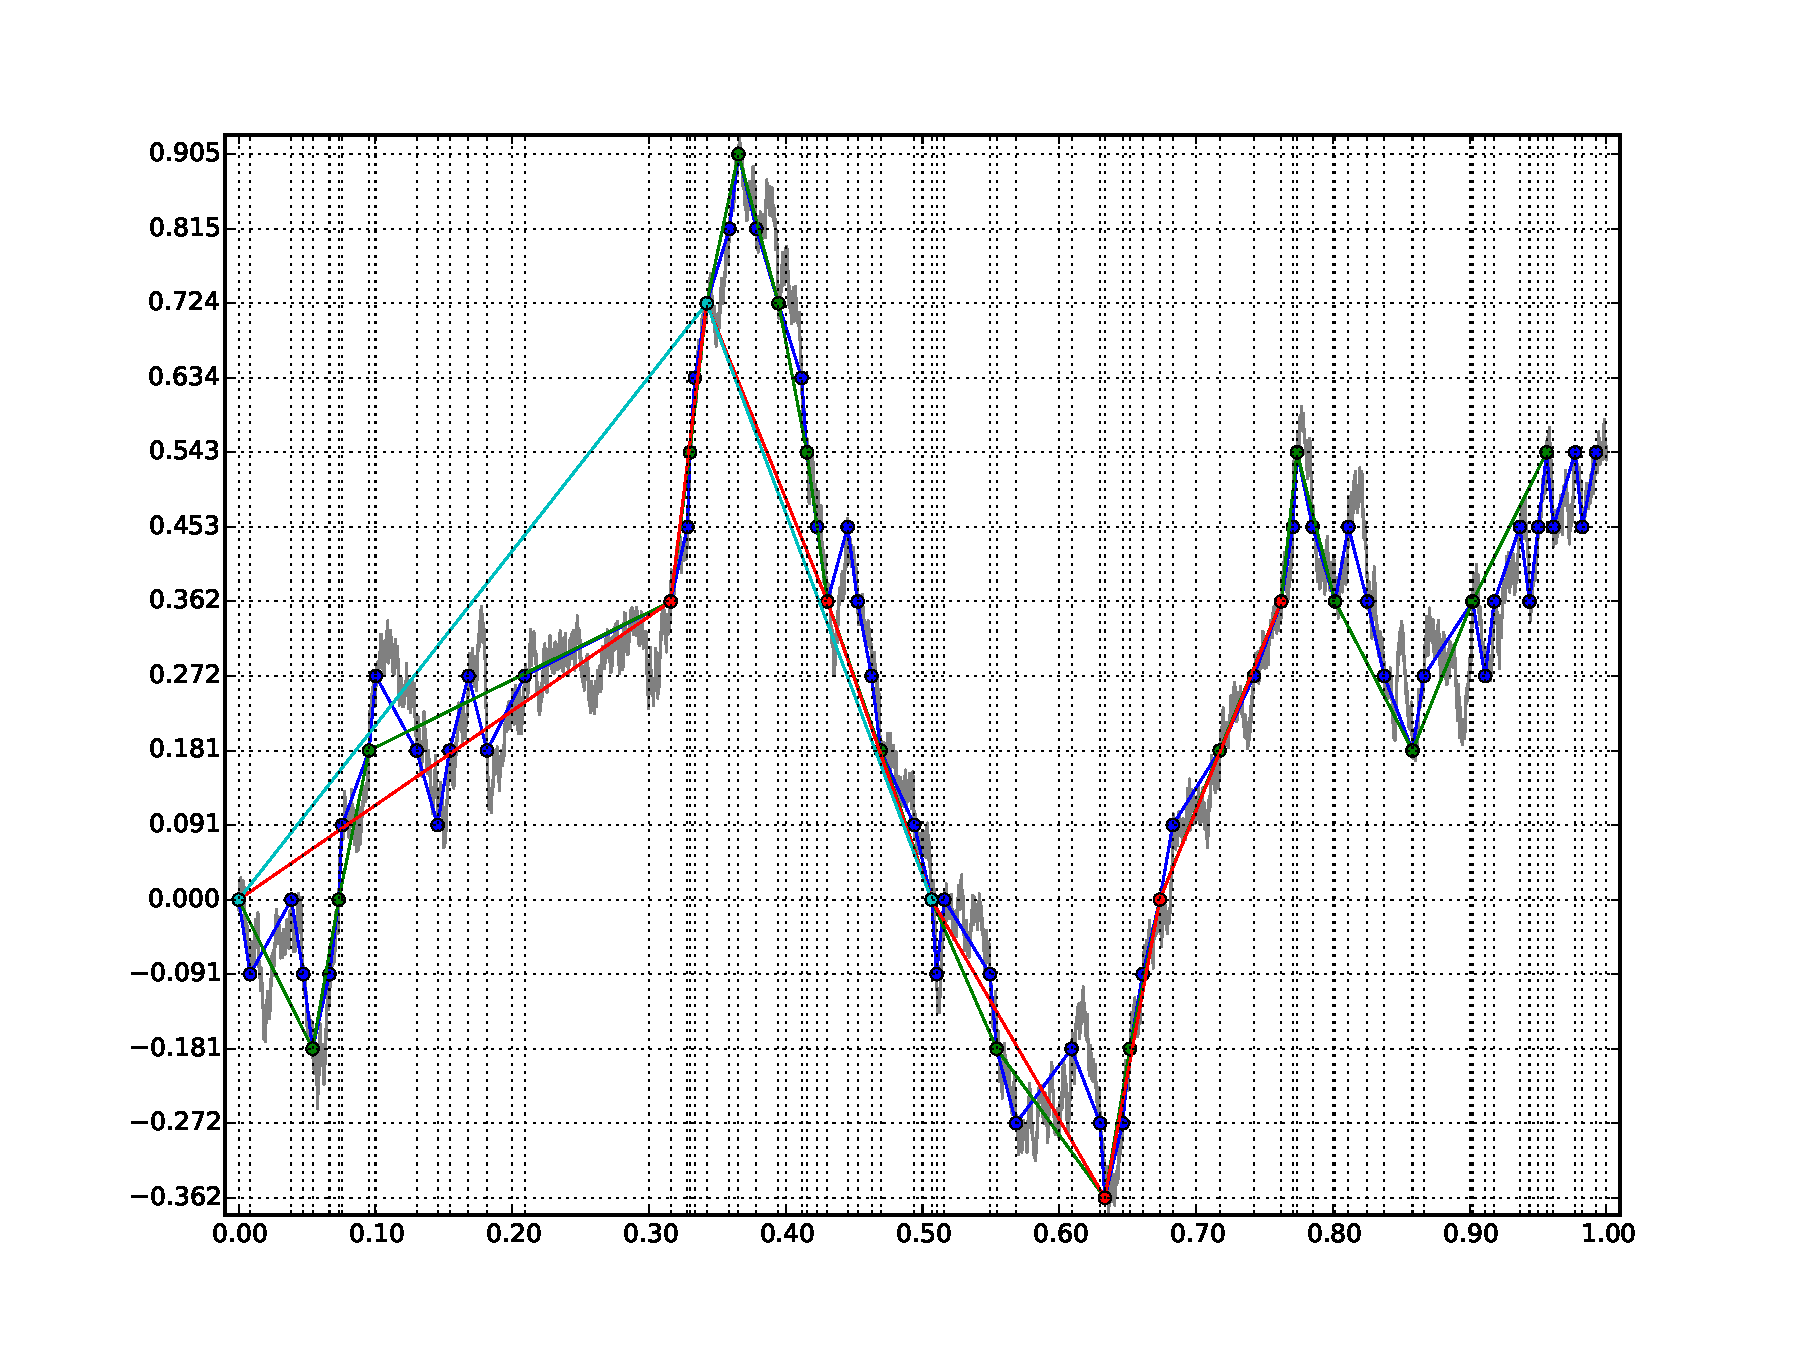
\includegraphics[draft,width=\linewidth]{../plots/sample_path.pdf}
    \end{subfigure}\\
    \vspace{-20pt}
    \begin{subfigure}{\linewidth}
        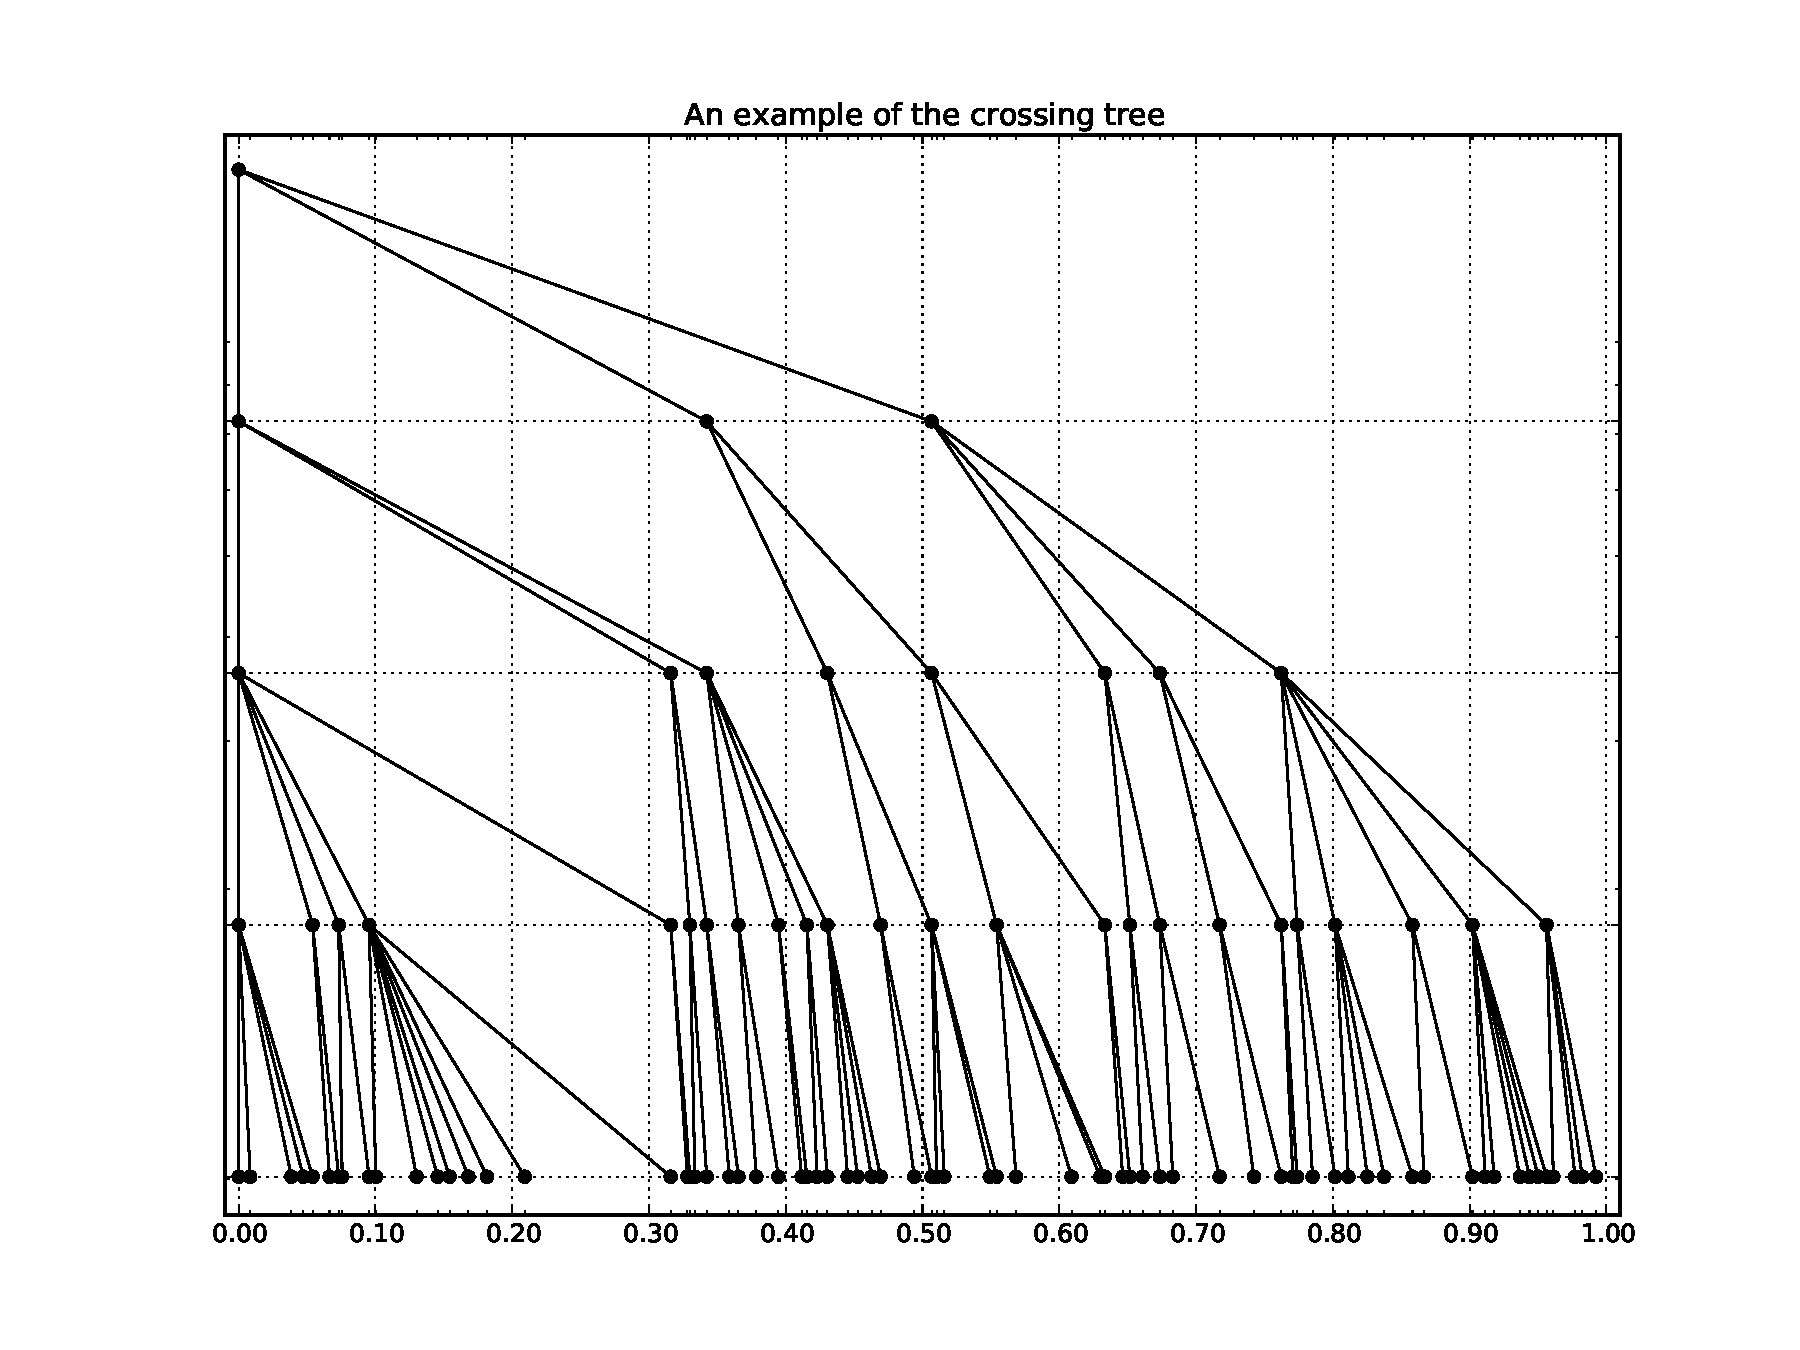
\includegraphics[draft,width=\linewidth]{../plots/sample_tree.pdf}
    \end{subfigure}
    \vspace{-10pt}
    \caption{\emph{top}: the crossing times and levels of a sample trajectory of
    a continuous process; \emph{bottom}: the corresponding crossing tree.}
    \label{fig:sample_tree}
    \vspace{-10pt}
\end{figure}

\subsection{Theoretical construction} % (fold)
\label{sub:theoretical_construction}

The $n$-th level crossing times are non-decreasing, but for continuous processes
$T_k^n < T_{k+1}^n$. We proceed by contradiction. By continuity of $X(t)$ at $T_k^n$
there is $\epsilon>0$ with $|X(t) - X(T_k^n)| < \frac{1}{2}\delta 2^n$ for all
$t\in [T_k^n, T_k^n + \epsilon)$. But by definition in the right $\epsilon$ vicinity
of $T_{k+1}^n$ there is a $t$ with $|X(t) - X(T_k^n)|\geq \delta 2^n$. Therefore,
if $T_k^n = T_{k+1}^n$, then there would be an $t$ for which $\delta 2^n < \frac{1}{2}\delta 2^n$,
which is a contradiction.

Another property is that $|X(T_{k+1}^n) - X(T_k^n)| = \delta 2^n$ when $T_{k+1}^n$
is finite. Indeed, the function $t \mapsto |X(t) - X(T_k^n)|$ is continuous at $T_{k+1}^n$,
whence $|X(T_{k+1}^n) - X(T_k^n)| \geq \delta 2^n$. We proceed by contradiction:
if $|X(T_{k+1}^n) - X(T_k^n)| > \delta 2^n$, then continuity implies that there is
$t\in (T_k^n, T_{k+1}^n)$ with $|X(t) - X(T_k^n)| > \delta 2^n$, which contradicts
the definition of $T_{k+1}^n$.
% not the greatest lower bound on all $s\geq T_k^n$ with $|X(s)-X(T_k^n)| \geq \delta 2^n$.

To summarize, the crossing times of a continuous process are such, that $T_k^n < T_{k+1}^n$,
$|X(T_{k+1}^n) - X(T_k^n)| = \delta 2^n$ for all $k\geq0$ with $T_{k+1}^n < +\infty$.

The halving of spatial resolution of any adjacent lattices permits a parent-child
relation between the corresponding crossings. Indeed, a child of an $m$-th $(n+1)$-st
level crossing is any $n$-th level crossing, a \emph{subcrossing}, which takes place
during it. The set of all \emph{offspring} subcrossings is given by
\begin{equation} \label{eq:crossing_offspring}
    J_{m+1}^{n+1}
        = \bigl\{ k \geq 0 \,:\,
            [T_k^n, T_{k+1}^n) \subseteq [T_m^{n+1}, T_{m+1}^{n+1})
        \bigr \} \,,
\end{equation}
with $J_0^{n+1} = \emptyset$. Furthermore, there necessarily is $k\geq 0$ such that
$T_m^{n+1} = T_k^n$, since $\delta 2^{n+1} \mathbb{Z} \subset \delta 2^n \mathbb{Z}$.
Note, that the parent crossing does not have to be complete ($T_{m+1}^{n+1} < \infty$)
for it to have subcrossings.

Let the number of complete $n$-he level crossings be $N_n = |\{k\geq 1\,:\, T_k^n < +\infty\}|$,
and $Z_k^n = \bigl| J_k^n \bigr|$ for $n\geq1$ and $k = 1,\ldots, N_n$ be the number
of subcrossings of the $k$-th complete $n$-th level crossing. Then $\sum_{k=1}^{N_{n+1}} Z_k^{n+1} \leq N_n$,
since there might be incomplete crossings.

There is a finer structure to the set of subcrossings of the $m$-th $(n+1)$-st level
crossing. If $k\geq 0$ is such that $T_k^n \in [T_m^{n+1}, T_{m+1}^{n+1})$ and
$X(T_m^{n+1}) = X(T_k^n)$, then for all $t \in [T_k^n, T_{k+1}^n)$
\begin{equation*}
    |X(t) - X(T_m^{n+1})| = |X(t) - X(T_k^n)| < \delta 2^n < \delta 2^{n+1} \,,
\end{equation*}
which implies that $t \leq T_{m+1}^{n+1}$. Therefore $T_{k+1}^n \leq T_{m+1}^{n+1}$.
Note that $T_{m+1}^{n+1} < +\infty$ implies $T_{k+1}^n < T_{m+1}^{n+1}$. Indeed,
if this is otherwise, then $X(T_m^{n+1}) = X(T_k^n)$, which contradicts continuity:
\begin{equation*}
    \delta 2^n = |X(T_{k+1}^n) - X(T_k^n)|
        = |X(T_{m+1}^{n+1}) - X(T_m^{n+1})| = \delta 2^{n+1}\,.
\end{equation*}
Furthermore $T_{k+2}^n \leq T_{m+1}^{n+1}$: the case $T_{m+1}^{n+1} = \infty$ is trivial,
but when the $m$-th $n+1$-st level crossing is complete we proceed by contradiction.
Indeed, the definition of $T_{k+2}^n$ implies that having $T_{m+1}^{n+1} < T_{k+2}^n$
would imply $|X(T_{m+1}^{n+1}) - X(T_{k+1}^n)| < \delta 2^n$. However finiteness
of $T_{m+1}^{n+1}$ implies $|X(T_{k+1}^n) - X(T_k^n)| = \delta 2^n$ and
$|X(T_{m+1}^{n+1}) - X(T_m^{n+1})| = \delta 2^{n+1}$. Hence the triangle inequality
and $X(T_m^{n+1}) = X(T_k^n)$ imply
\begin{align*}
    \delta 2^{n+1}
        &= \bigl|X(T_{m+1}^{n+1}) - X(T_m^{n+1})\bigr| \\
        &\leq \bigl|X(T_{m+1}^{n+1}) - X(T_{k+1}^n)\bigr|
           + \bigl|X(T_{k+1}^n) - X(T_k^n)\bigr| \\
        &< \delta 2^n + \delta 2^n \,.
\end{align*}
Therefore $X(T_m^{n+1}) = X(T_k^n)$ and $T_k^n \in [T_m^{n+1}, T_{m+1}^{n+1})$ imply
\begin{equation} \label{eq:duration_partition}
    \bigl[T_k^n, T_{k+1}^n\bigr) \cup \bigl[T_{k+1}^n, T_{k+2}^n\bigr)
        \subseteq \bigl[T_m^{n+1}, T_{m+1}^{n+1}\bigr)
    \,.
\end{equation}

%% A simple illustration of the movements within one crossing
\begin{figure}
    \centering
    \resizebox{\linewidth}{!}{
        \tikzset{bullet/.style={circle,draw, fill=black,minimum size=5pt,inner sep=0pt},}
        \begin{tikzpicture}[grow=right, sloped]
    %% Crossings
            \node [bullet] (o) {};
            \node [bullet] (u) [above right = 3em and 9em of o.west, anchor = west] {};
            \node [bullet] (d) [below right = 3em and 9em of o.west, anchor = west] {};
            \node [bullet] (uu) [above right = 3em and 9em of u.west, anchor = west] {};
            \node [bullet] (ud) [above right = 3em and 9em of d.west, anchor = west] {};
            \node [bullet] (dd) [below right = 3em and 9em of d.west, anchor = west] {};
    %% The anchor and labels
            \node [draw=none] [left = 0em of o.west, anchor = east] {$X(T_k^n)$};
            \node [draw=none] [right = 0em of ud.east, anchor = west] {$X(T_k^n) = X(T_{k+2}^n)$};
            \node [draw=none] [right = 0em of uu.east, anchor = west] {$X(T_k^n) + 2 \delta 2^n$};
            \node [draw=none] [right = 0em of dd.east, anchor = west] {$X(T_k^n) - 2 \delta 2^n$};
            \node [draw=none] [left = 0em of u.west, anchor = south east] {$X(T_k^n) + \delta 2^n$};
            \node [draw=none] [left = 0em of d.west, anchor = north east] {$X(T_k^n) - \delta 2^n$};
    %% Crossing times nodes at the bottom
            \node [draw=none] (t2) [below = 1.25em of dd.south, anchor = west] {$T_{k+2}^n$};
            \node [draw=none] (t1) [left = 9em of t2.west, anchor = west] {$T_{k+1}^n$};
            \node [draw=none] (t0) [left = 9em of t1.west, anchor = west] {$T_k^n$};
    %% Dumy nodes on the top level
            \node [fill=none,draw=none] (dummy2) [above = 1em of uu.north, anchor = north] {};
            \node [fill=none,draw=none] (dummy1) [left = 9em of dummy2.west, anchor = west] {};
            \node [fill=none,draw=none] (dummy0) [left = 9em of dummy1.west, anchor = west] {};
    %% Paths to levels
            \path[thick,draw]
                (o) edge node[above] {$+\delta 2^n$} (u)
                (o) edge node[below] {$-\delta 2^n$} (d)
                (u) edge node[above] {$+\delta 2^n$} (uu)
                (u) edge node[below] {$-\delta 2^n$} (ud)
                (d) edge node[above] {$+\delta 2^n$} (ud)
                (d) edge node[below] {$-\delta 2^n$} (dd);
    %% Crossing times
            \draw[black, dashed] (dummy2.west -| t2.west) -- (t2.west -| t2.west) {};
            \draw[black, dashed] (dummy1.west -| t1.west) -- (t1.west -| t1.west) {};
            \draw[black, dashed] (dummy0.west -| t0.west) -- (t0.west -| t0.west) {};
        \end{tikzpicture}
    }
    %% A very informative caption
    \caption{Possible traversals over $t\in \bigl[T_k^n, T_{k+2}^n\bigr)$ for a
    continuous process.}
    \label{fig:xing_tree_structure}
    \vspace{-10pt}
\end{figure}

Another important observation is that any complete crossing has an even number of
subcrossings in \eqref{eq:crossing_offspring}. Indeed, if $T_k^n = T_m^{n+1}$ and
$T_{m+1}^{n+1} < +\infty$, then there is an integer $p > 0$ with $T_{k+p}^n = T_{m+1}^{n+1}$.
However, \eqref{eq:duration_partition} implies that there are two possibilities at
$T_{k+2}^n$:
\begin{enumerate}
    \item the path crossed a level other than $X(T_k^n)$, inducing a crossing of
    $\delta 2^{n+1}\mathbb{Z}$ lattice;
    \item the path returned to $X(T_k^n)$ level, in which case $X(T_{k+2}^n) = X(T_m^{n+1})$
    and thus by the time $T_{k+2}^n$ no $(n+1)$-st level crossing occurred.
\end{enumerate}
In the former case $T_{m+1}^{n+1} \leq T_{k+2}^n$ and thus $p=2$, while in the latter
case this argument can be repeated for $k \leftarrow k+2$. Hence there is a $q > 0$
with $p = 2q + r$, $r \in \{0, 1\}$, and
\begin{equation*} \label{eq:subcrossing_partition}
    \bigcup_{j=0}^{q-1} \bigl[T_{k+2j}^n, T_{k+2j+1}^n\bigr)
                   \cup \bigl[T_{k+2j+1}^n, T_{k+2j+2}^n\bigr)
        \subseteq \bigl[T_m^{n+1}, T_{m+1}^{n+1}\bigr) \,.
        \tag{\ref{eq:duration_partition}'}
\end{equation*}
Note, that $r\neq 1$, since over $\bigl[T_{k'}^n, T_{k'+1}^n\bigr)$, $k' = k + 2q$,
a continuous process necessarily moves $\pm \delta 2^n$, (fig.~\ref{fig:xing_tree_structure}).
Therefore $\bigl| J_{m+1}^{n+1} \bigr| = p = 2q$.

By \eqref{eq:subcrossing_partition} subcrossings of a complete crossing are paired,
and the last pair always has the same orientation, which concludes the parent crossing
by hitting $\delta 2^{n+1} \mathbb{Z}$. Thus complete crossings can be broken into
a series of \emph{excursions} -- pairs of oppositely oriented subcrossings within
$\pm\delta 2^n$ levels, followed by a psir of indentically oriented subcrossings.
Let $V_k^n$ be the movement pattern of the $k$-th $n$-th level excursion: either
`+-' for up-down, or `-+' for down-up movements.

% subsection theoretical_construction (end)

\subsection{Practical construction} % (fold)
\label{sub:practical_construction}

The tree is built from the crossings at the finest scale $\delta > 0$ by gradually
halving the resolution, until no complete crossings occur. To this end the univariate
time series $(t_i, x_i)_{i=1}^m$ is interpolated by a piecewise linear continuous
trajectory $X(t)$, with static values outside of $[t_1, t_m]$. This interpolation
implies that the $n$-th level crossing times \eqref{eq:xing_time} by the intersections
of the linear segments with lines of the lattice $\delta 2^n \mathbb{Z}$, which
are not immediately preceded by a crossing of the same lattice line. This procedure
has linear time and memory complexity in output size: $\mathcal{O}(N_n)$ where $N_n$
is the number of complete crossings $N_n = |\{k\geq 1\,:\, T_k^n < +\infty\}|$.

Once the crossing times for all resolutions are computed, the offspring of level
$n+1$ crossings is determined directly by \eqref{eq:crossing_offspring}. For this
its sufficient to find locations, at which the times $(T_k^n)_{k=1}^{N_n}$ should
be inserted into $(T_m^{n+1})_{m=1}^{N_{n+1}}$ to keep the latter sorted, up to
numerical accuracy. In fact this alignment can be done in a single pass through
the $n$-th level crossing times, and thus has complexity $\mathcal{O}(N_n)$.

Since \eqref{eq:subcrossing_partition} implies that each new level of the tree has
no more than half of the crossings of the preceding level, and each level is visited
only once, the complexity of the crossing tree construction is $\mathcal{O}(N_0)$,
where $N_0$ is the number of crossings of the finest lattice $\delta \mathbb{Z}$.
In turn, $N_n$ can be upper bounded by the ratio of the total absolute variation
of the path to the scale. For time series data $(t_i, x_i)_{i=1}^m$ with increments
$\Delta_i = x_i - x_{i-1}$ we have $N_n \leq (\delta 2^n)^{-1} \sum_{i=1}^m |\Delta_i|$.

In addition to the construction complexity of the tree, the choice of $\delta > 0$
affects its depth and how well each level is populated by crossings. For relatively
small $\delta$ the crossing tree will be quite deep, but its lower levels will be
overcrowded by short crossings, since at high resolutions the path is a series of
direct upward or downward movements. On the other hand, a large $\delta$ produces
a shallow tree with less discretization bias, but underpopulated \emph{offspring}
distribution within each level, which could lead to provide less reliable estimates
of scale invariance.

The base scale $\delta$ can be picked adaptively: by either the standard deviation
or the inter-quartile range of the increments, or the mean or the median of their
absolute values.

% subsection practical_construction (end)

% section the_crossing_tree (end)

\section{Characterization with the crossing tree} % (fold)
\label{sec:characterization_with_the_crossing_tree}

The crossing tree produces a set of characteristics, which in some cases uniquely
identify certain continuous stochastic processes, \cite{ECP1673}. One such process
in the Brownian Motion (BM) -- a unique zero-mean Gaussian process with covariance
kernel $R(s,t)=\min\{s, t\}$ and almost surely continuous paths starting at the origin.
In \cite{ECP1673} it is shown that BM is a unique continuous process starting at
the origin with the following properties:
\begin{itemize}
    \item each level has infinitely many offspring ($N_n = +\infty$);
    \item the scaled crossing durations $(\delta 2^n)^{-\frac{1}{H}} W_k^n$
    are independent within each level and identically distributed with mean $1$
    and finite variance;
    \item the number of subcrossings $Z_k^n$ is iid with
    \begin{equation}\label{conj:subcross}
        \pr(Z_k^n = 2m) = \theta_H (1 - \theta_H)^{m-1} \,,
    \end{equation}
    with $\theta_H = 2^{1 - H^{-1}}$ for integer $m\geq 1$;
    \item the excursion directions $V_k^n$ are independent of the parent crossing
    directions and iid with $\pr(V_k^n=\text{`+-'}) = 2^{-2 H^{-1}}$;
\end{itemize}
where $H = \frac{1}{2}$. This characterisation is based on the construction of the
BM on a nested fractal in \cite{BarlowPerkins88}. Furthermore the BM is an example
of an $H$-self similar process with stationary increments having $H=\frac{1}{2}$.

It seems plausible that parts of this characterisation can be extended to Gaussian
$H$-sssi processes with $H \in(\frac{1}{2}, 1)$. Indeed, \cite{jonesshen2005} show
that if the process is continuous, self-similar and has stationary and ergodic increments,
then the sequences of the number of subcrossings $Z^n = (Z_k^n)_{k\geq 0}$ are identically
distributed across levels, and stationary and ergodic within each level. The same
result holds for scaled crossing durations. Therfore, we conjecture that for $H$-sssi
(sec.~\ref{sec:self_sim_processes}) processes the crossing tree has these statistical
properties:
\begin{description}
    \item[C1] conditioning on the parent crossing, $V_k^n$ have distribution
    $\pr(V_k^n = \text{`+-'}|\text{`+'}) = \pr(V_k^n = \text{`-+'}|\text{`-'}) = 2^{-2 H^{-1}}$;
    \item[C2] $Z_k^n$ are distributed as \eqref{conj:subcross}, but possibly correlated;
    \item[C3] $(\delta 2^n)^{-\frac{1}{H}} W_k^n$ are identically distributed with mean $1$.
\end{description}
This conjecture makes it possible to use the crossing tree to estimate $H$ based
on the offspring distribution and mean durations: $H^{-1} \approx \log_2 \ex Z^n$,
or $H^{-1} \approx \log_2 \frac{\ex W^{n+1}}{\ex W^n}$. 

In sec.~\ref{sec:experiment} we conduct an extensive simulation study on Gaussian
and non-Gaussian $H$-sssi processes, reviewed in sec.~\ref{sec:self_sim_processes},
to test plausibility of the conjecture.

% section characterization_with_the_crossing_tree (end)

\section{Typical self-similar processes} % (fold)
\label{sec:self_sim_processes}

In the simulation study we consider continuous monofractal real-valued stochastic
processes: Gaussian and Hermite $H$-sssi processes (sec.~\ref{sub:h_sssi_proc}),
and the Weierstrass function (sec.~\ref{sub:weierstrass_function}).

\subsection{Gaussian and Hermite $H$-sssi processes} % (fold)
\label{sub:h_sssi_proc}

A process $(X(t))_{t\geq0}$ is $H$-self similar (or $H$-\textbf{ss}) if for all $a>0$
\begin{equation*} \label{eq:def_ss}
    (X(at))_{t\geq0} \overset{\Dcal}{\sim} (a^H X(t))_{t\geq0} \,,
\end{equation*}
understood as equality of all finite dimensional distributions. A process is said
to have stationary increments (\textbf{si}) if
\begin{equation*}\label{eq:def_si}
    (X(t)-X(s))_{t\geq0} \overset{\Dcal}{\sim} (X(t-s)-X(0))_{t\geq0} \,,
\end{equation*}
for any $s\geq 0$. If $(X(t))_{t\geq0}$ is $H$-ss then $X(t) \overset{\Dcal}{\sim} t^H X(1)$
for any $t>0$, and if, in addition, it has zero mean and stationary increments, then
its covariance function is given by
\begin{align}\label{eq:h_sssi_cov}
    \ex X(t) X(s)
        &= \frac{1}{2} \bigl(\ex X(s)^2 + \ex X(t)^2 - \ex(X(s) - X(t))^2 \bigr) \nonumber \\
        % &= \frac{1}{2} \bigl( s^{2H} \ex X(1)^2 + t^{2H}\ex X(1)^2 - \ex(X(|s-t|))^2 \bigr) \\
        &= \frac{1}{2} (s^{2H}  + t^{2H} - |s-t|^{2H}) \ex X(1)^2 \,.
\end{align}

A stochastic process $(X(t))_{t\geq0}$ is Gaussian with mean $\mu(t)$ and covariance
kernel $R(s,t)$ (positive definite function) if for any $n\geq 1$, $0 \leq t_i < t_{i+1}$
with $i=1,\ldots,n$, the vector $(X(t_i))_{i=1}^n\in \Real^{n\times1}$ is $n$-dimensional
Normal with mean $(\mu(t_i))_{i=1}^n$ and covariance matrix $(R(t_i, t_j))_{i,j=1}^n\in \Real^{n\times n}$.
Now, the Brownian Motion (BM) process $(B(t))_{t\geq0}$ is a zero-mean Gaussian process
with $X(0)=0$ and almost surely continuous paths such that its covariance kernel is
$R(s,t)=\min\{s, t\}$. Gaussianity and covariance structure imply that BM is an $H$-sssi
process for $H=\frac{1}{2}$, since for any $a>0$ the process $(a^{-\frac{1}{2}} B_{at})_{t\geq0}$
is just another version of the BM.

Fractional Brownian motion (fBM) -- a generalization of the BM to an $H$-sssi Gaussian
process for $H \in (\frac{1}{2}, 1)$, -- was introduced in \cite{doi:10.1137/1010093}.
Formally, fBM, denoted by $(B_H(t))_{t\geq0}$, is a continuous zero-mean Gaussian
process with stationary increments and the covariance kernel given by \eqref{eq:h_sssi_cov}.
This class of processes exhausts all Gaussian $H$-sssi processes, \cite{embrechts2002},
and has an It\^o integral representation with respect to the BM $(W_x)_{x\in\Real}$
\begin{equation}\label{eq:fbm_int_repr}
    B_H(t) = C \int_\Real \biggl(
            \int_0^t (u-x)_+^{H-\frac{3}{2}} {du}
        \biggr) {dW_x} \,,
\end{equation}
for a normalising constant $C$, which depends on $H$.

fBM processes, are a particular instance of a class of generally non-Gaussian $H$-sssi
processes, called the \textbf{Hermite} processes, named after the stochastic integral
kernel used in its definition. It is an important class of non-Gaussian self-similar
processes, \cite{maejima2007}. The $H$-sssi Hermite process $(Z_H^m(t))_{t\geq 0}$
of order $m$, $H \in (\frac{1}{2}, 1)$, is defined as % multiple Wiener-It\^o integral
% of order $m$ with respect to the standard BM $(W_t)_{t\geq0}$:
\begin{equation}\label{eq:def_hermite}
    Z_H^m(t) = C \int_{\Real^m}' \Biggl(
            \int_0^t \prod_{k=1}^m (u - x_k)_+^{H_0-\frac{3}{2}} du
        \Biggr) dW_{x_1} \ldots dW_{x_m}\,,
\end{equation}
where $H = m (H_0-1)+1$, $C$ is a normalising constant, and $\int_{\Real^m}'$ is an
$m$-dimensional integral over $\Real^m$ excluding the diagonals. For $m=1$ the Hermite
process is the fBM \eqref{eq:fbm_int_repr}, but for $m\geq 1$ higher order Hermite
processes correspond to non-Gaussian $H$-sssi,
\cite{Bai20141710,Chronopoulou:1114288,embrechts2000introduction}.
% http://samm.univ-paris1.fr/Sofwares-Logiciels

% subsection h_sssi_proc (end)

\subsection{Weierstrass function} % (fold)
\label{sub:weierstrass_function}

An example of a non $H$-sssi process, which has scale invariance is the Weierstrass
function, \cite{decrouez2013}. This process $W_H:[0,1] \mapsto \Real$ has continuous,
nowhere differentiable paths, and is defined as the trigonometric series:
\begin{equation} \label{eq:def_weir}
    W_H(t) = \sum_{k\in \mathbb{Z}} \lambda_0^{-k H} \bigl(
            \cos(2\pi \lambda_0^k t + \phi_k) - \cos \phi_k
        \bigr) \,,
\end{equation}
where $H\in(0, 1)$, the phase shifts $(\phi_k)_{k\in\mathbb{Z}}$ are iid uniformly
random over $[0, 2\pi]$, and $\lambda_0 > 1$ is the \emph{fundamental harmonic}.

This process has discrete scale invariance ($W_H(\lambda_0 t) \overset{\Dcal}{\sim} \lambda_0^H W_H(t)$,
\cite{decrouez2015}), and is H\"older continuous with exponent $H$: there is $C \geq 0$
such that
\begin{equation} \label{eq:def_holder}
    \bigl| W_H(s) - W_H(t) \bigr| \leq C |s - t|^H \,,
\end{equation}
that for all $s,t\geq [0,1]$. Indeed, a trigonometric identity for difference of
cosines involving angles $2\pi \lambda_0^k t + \phi_k + \pi \lambda_0^k \Delta$
and $\pi \lambda_0^k \Delta$ implies that for any $\Delta$ we have
\begin{equation*}
    \bigl| W_H(t+\Delta) - W_H(t) \bigr|
        \leq 2 \sum_{k\in \mathbb{Z}} \lambda_0^{-k H} |\sin(\pi \lambda_0^k \Delta)| \,.
\end{equation*}
If $K^+_\Delta = \inf\{k\geq 1\,:\, \lambda_0^k |\Delta| \geq 1\}$ and $K^-_\Delta$
is the least $k\geq 1$ with $\lambda_0^{-k} |\Delta| \leq 1$, then by breaking up
the right-hand series at indices $k\in\{-K^-_\Delta, 0, K^+_\Delta\}$, and using
$|\sin \theta| \leq |\theta|$, it can be seen that the variation is upper bounded
by $C(\lambda_0, H) |\Delta|^H$.

% subsection weierstrass_function (end)

\subsection{Simulation of the processes} % (fold)
\label{sub:simulation_of_the_processes}

The usual method for generating a sample of the fractional Gaussian Noise is through
the Cholesky decomposition of the covariance matrix, which has complexity $\mathcal{O}(N^2)$,
where $N$ is the length of the sample. This is sufficient for small samples, but
in order to have better approximations of continuous processes it is necessary to
use very large $N$. One viable alternative is to use the Circulant Embedding Method
which has $\mathcal{O}(N \log N)$ complexity, \cite{WRCR:WRCR6232}. This method
proceeds by factorizing a special embedding of the correlation matrix to produce
random vectors with exact correlation structure of the fractional Gaussian Noise
via the Fourier Transform, \cite{Perrin:1058211}.

All processes in this study are sampled on a regular grid $(t_k)_{i=0}^N$ in $[0,1]$
with spacing $\Delta=\frac{1}{N}$, and $t_i = i \Delta$. On this grid sample paths
of the fractional Brownian Motion can be generated by integrating the fGN with variance
$\Delta^\frac{1}{H}$. The Hermite processes are generated based on the Non Central
Limit Theorem, \cite{embrechts2002,tudor2008}, which states that if $(\xi_k)_{k\geq0}$
is a centered stationary Gaussian sequence with $\ex\xi_k^2=1$ and
$\ex \xi_k \xi_0 \approx C |k|^\frac{2H-2}{m}$ for large $k$ and $H\in(\frac{1}{2}, 1)$,
then
\begin{equation*}
    \biggl(\frac{1}{n^H} \sum_{j=1}^{\lfloor n t\rfloor}
        H_m(\xi_j)\biggr)_{t\geq0} 
            \overset{\Dcal}{\longrightarrow} \bigl(Z_H^m(t)\bigr)_{t\geq0} \,,
\end{equation*}
as $n\to\infty$, where $H_m(x) = (-1)^m e^\frac{x^2}{2}\frac{d^m}{dx^m}e^{-\frac{x^2}{2}}$
is the Hermite polynomial of degree $m$. The sequence $(\xi_k)_{k\geq0}$ can be sampled
from the fractional Gaussian Noise with Hurst index $H_0 = \frac{H-1}{m}+1$ as in
\eqref{eq:def_hermite}, \cite{embrechts2000introduction}.

Sample paths of the Weierstrass function are approximated by truncating \eqref{eq:def_weir}
at $|k| \leq 1+\bigl\lfloor \log_{\lambda_0} \frac{N}{2} \bigr\rfloor$, which ensures
that the harmonics are adequately sampled over the grid, \cite{decrouez2013}.

% subsection simulation_of_the_processes (end)

% section self_sim_processes (end)

\section{Setup and results} % (fold)
\label{sec:experiment}

In order to gather empirical evidence either supporting or refuting this claim,
extensive numerical study was in order. The Monte-Carlo simulation was performed
on each of the processes mentioned in the previous chapter (p.~\pageref{sec:self_sim_processes}).
The software part of the experiment was implemented in Python in conjunction with
Numpy \cite{harris_array_2020} and FFTW \cite{gomersall_pyfftw_2016}, a standalone
open source library dedicated to efficiently computing Fast Fourier Transforms.%
%
\footnote{
    The source code of the experiment is available at
    \url{https://github.com/ivannz/crossing_paper2017}
}

\subsection{Analysis using the crossing tree} % (fold)
\label{sub:analysis_using_the_crossing_tree}

For each sample path of the process we construct the crossing tree, which yields
the offspring $(Z_k^n)$, excursions $(V_k^n)$ and duration $(W_k^n)$ observations.
Provided the levels are well sampled, we can test the offspring distribution properties:
\cite{ECP1673}, it is reasonable to
expect that the offspring distributions of crossings of consecutive
levels of the tree are identical.

\begin{enumerate}
    \item consider $h$ bins: $\{2m\}_{m=1}^{h-1}$ and $\{2h, 2h+2,\ldots\}$;
    \item compute the empirical probabilities $\hat{p}_k^n$ of the number of
    offspring $(Z_k^n)$ in each bin at every level from $p$ to $q$;
    \item pool all the offspring $Z_k^n$ at levels from $p$ to $q$ and compute
    the empirical distribution $\bar{p}_i$ over the bins;
    \item provided each bin is sufficiently populated, the hypothesis of identical
    distribution across levels can be tested with a standard $\chi^2$ test:
    \begin{equation*}
        t^{(p,q)} = \sum_{n=p}^q \sum_{k=1}^h N_n
            \frac{(\hat{p}_k^n - \bar{p}_k)^2}{\bar{p}_k}
            \sim \chi^2_{(q-p)(h-1)}
            \,.
    \end{equation*}
\end{enumerate}

Another characteristic of the process is the distribution of excursion patterns within
a parent crossing, conditional on its direction. Indeed, subcrossing orientations
of a complete crossing come in

% subsection analysis_using_the_crossing_tree (end)

\subsection{Results} % (fold)
\label{sub:results}

The crossing trees were constructed for a base scale $\delta$ dependent on each particular
sample realisation of the process, but in such a way as to enable meaningful comparisons
of the crossing tree properties between different Monte-Carlo replications and between
different classes of $H$-sssi processes. For a particular sample path $(x_j)_{j=0}^N$
of the process $\{X(t)\}$ the base scale was set to
\[ \delta = \text{med}\bigl( |\Delta x_j| \bigr) \,, \]
where $\Delta x_j = x_j - x_{j-1}$ and $\text{med}(\cdot)$ is the median of the
sample. The rationale behind the median of absolute increments of the sample path
was to strike a balance between the biasedness of the crossing tree parameters,
resulting from linear interpolation of the crossing times and the inaccuracy due to
too coarse a resolution. Other choices for the base scale were considered, such
as the standard deviation and the \textbf{i}nter\textbf{q}uartile \textbf{r}ange
measure of statistical dispersion of the increments. Neither did produce any significantly
different results from the median, except only that they tended to produce trees with
fewer levels and thus cover a narrower range of resolutions of the process.

It seems natural to begin with the study of the fractional Brownian motion. To this end,
$10^3$ Monte-Carlo simulations of sample paths of the fBM process were simulated. The
process was confined to the unit interval and discretized to have $2^{21}$ sample points.

Before proceeding to the evaluation of statistical properties of the crossing trees,
it is necessary to determine the range of tree levels (grid scales, or resolutions)
for which self-similarity is apparent.
\begin{figure}[htb]\begin{center}
    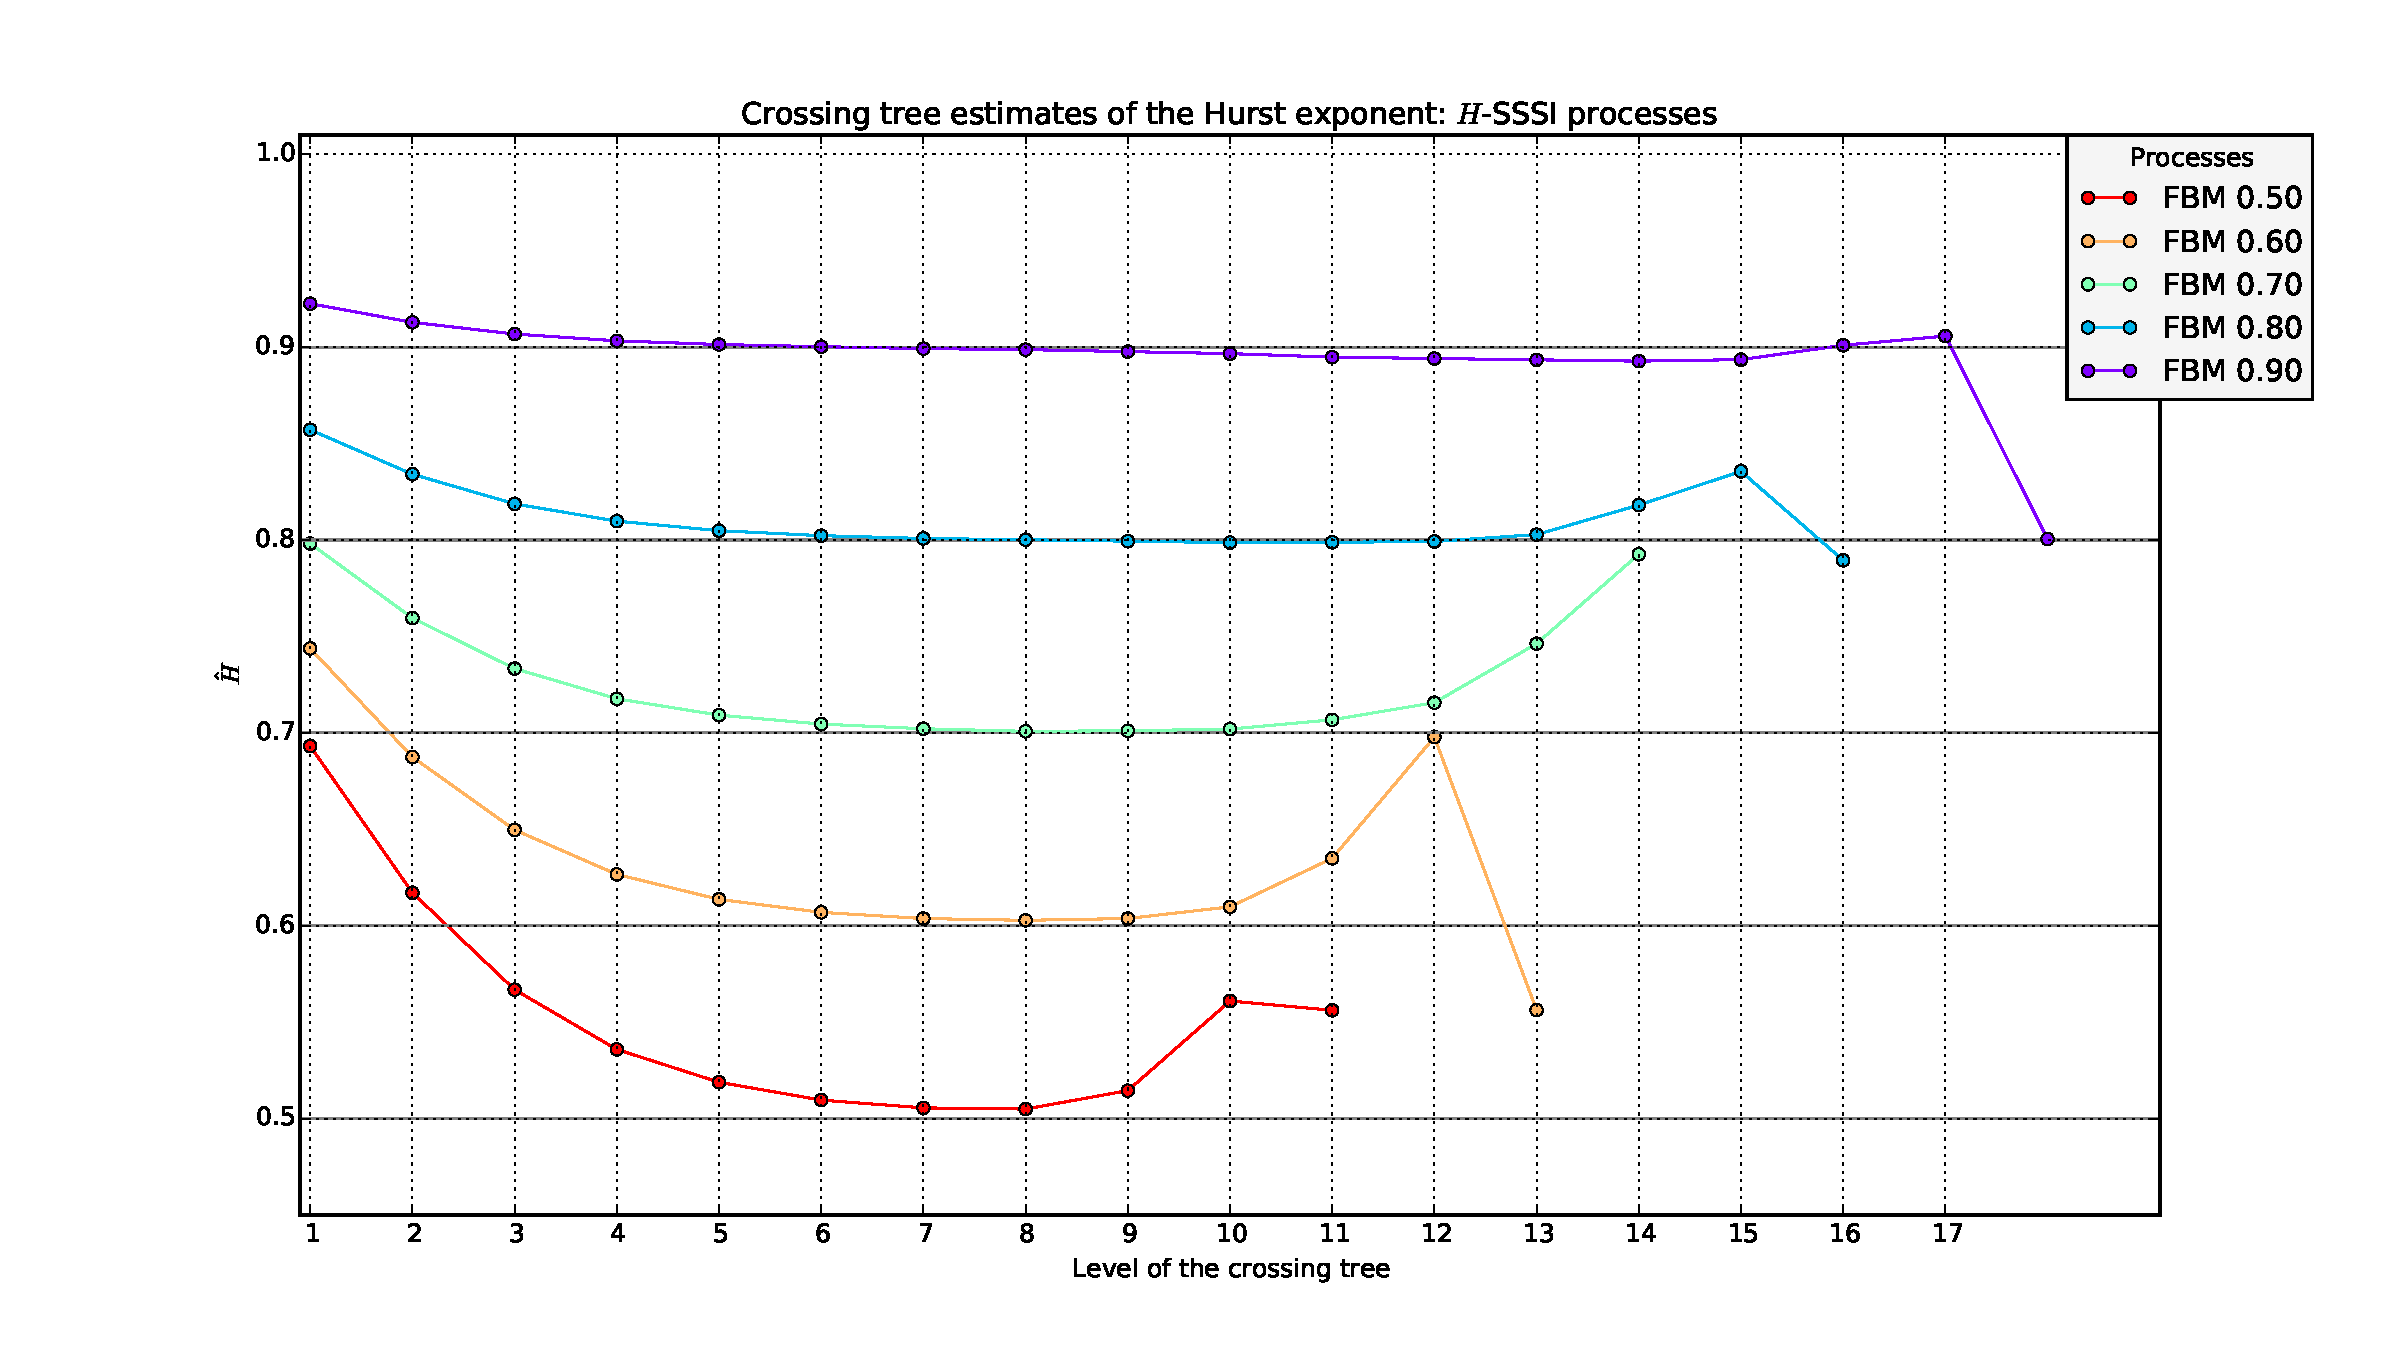
\includegraphics[draft,width=6in]{images/fbm_fig_05_med_1000-21}
    \caption{The plot of the estimates of the Hurst index $H$ on the offspring data
    of a single level of the crossing tree based on $10^3$ Monte-Carlo simulations of
    fBM.}
\label{fig:fbm_hurst_crossing_tree}
\end{center}\end{figure}

Figure~\ref{fig:fbm_hurst_crossing_tree} suggests that scale invariance properties
for the studied fractional processes and the chosen method of computation of the
base scale manifest their effects at across levels from 6 to 9. In fact the $\chi^2$
test described in section~\ref{sub:analysis_using_the_crossing_tree} does not seem
to support this finding and instead has the lowest empirical rejection rate exactly
at levels from 7 to 8 (see table~\ref{tbl:chi_sq_test_for_fbm_only}).
\begin{table}[h]\begin{center}
	\begin{tabular}{l||c|c|c|c|c|c|}
	Process 		&  $6-7$ &          $7-8$ & $8-9$ &  $6-8$ &  $7-9$ &  $6-9$ \\ \hline\hline
	fBM-$0.50$ 		& $10.6$ & $\mathbf{8.2}$ & $9.1$ & $13.6$ & $12.2$ & $16.2$ \\ \hline 
	fBM-$0.60$ 		& $10.9$ & $\mathbf{9.1}$ & $9.4$ & $14.2$ & $13.1$ & $16.4$ \\ \hline 
	fBM-$0.70$ 		&  $9.4$ & $\mathbf{7.0}$ & $7.2$ & $12.6$ & $11.2$ & $15.8$ \\ \hline 
	fBM-$0.80$ 		& $10.3$ & $\mathbf{6.1}$ & $6.7$ & $12.8$ & $10.7$ & $16.9$ \\ \hline 
	fBM-$0.90$ 		& $11.1$ & $\mathbf{7.8}$ & $7.9$ & $18.0$ & $12.8$ & $27.7$ \\ \hline 
 	\end{tabular}
	\caption{The table of empirical rejection rate at significance level of $\alpha = 5\%$
	of the $\chi^2$ test for self-similarity between levels of the crossing tree. }
\label{tbl:chi_sq_test_for_fbm_only}
\end{center}\end{table}
Since the self-similarity of the simulated fractional Brownian motion paths seems
to become apparent at levels 7 and 8 on average, we pool the crossing tree data of
these levels in order to obtain more reliable estimates.

Restricting the attention to the Brownian motion case (fBM with $H=\frac{1}{2}$)
one can easily see that the numerical evidence is well aligned with the theoretical
result of Jones and Rolls (fig.~\ref{fig:fbm_offspring_distribution}).
\begin{figure}[htb]\begin{center}
    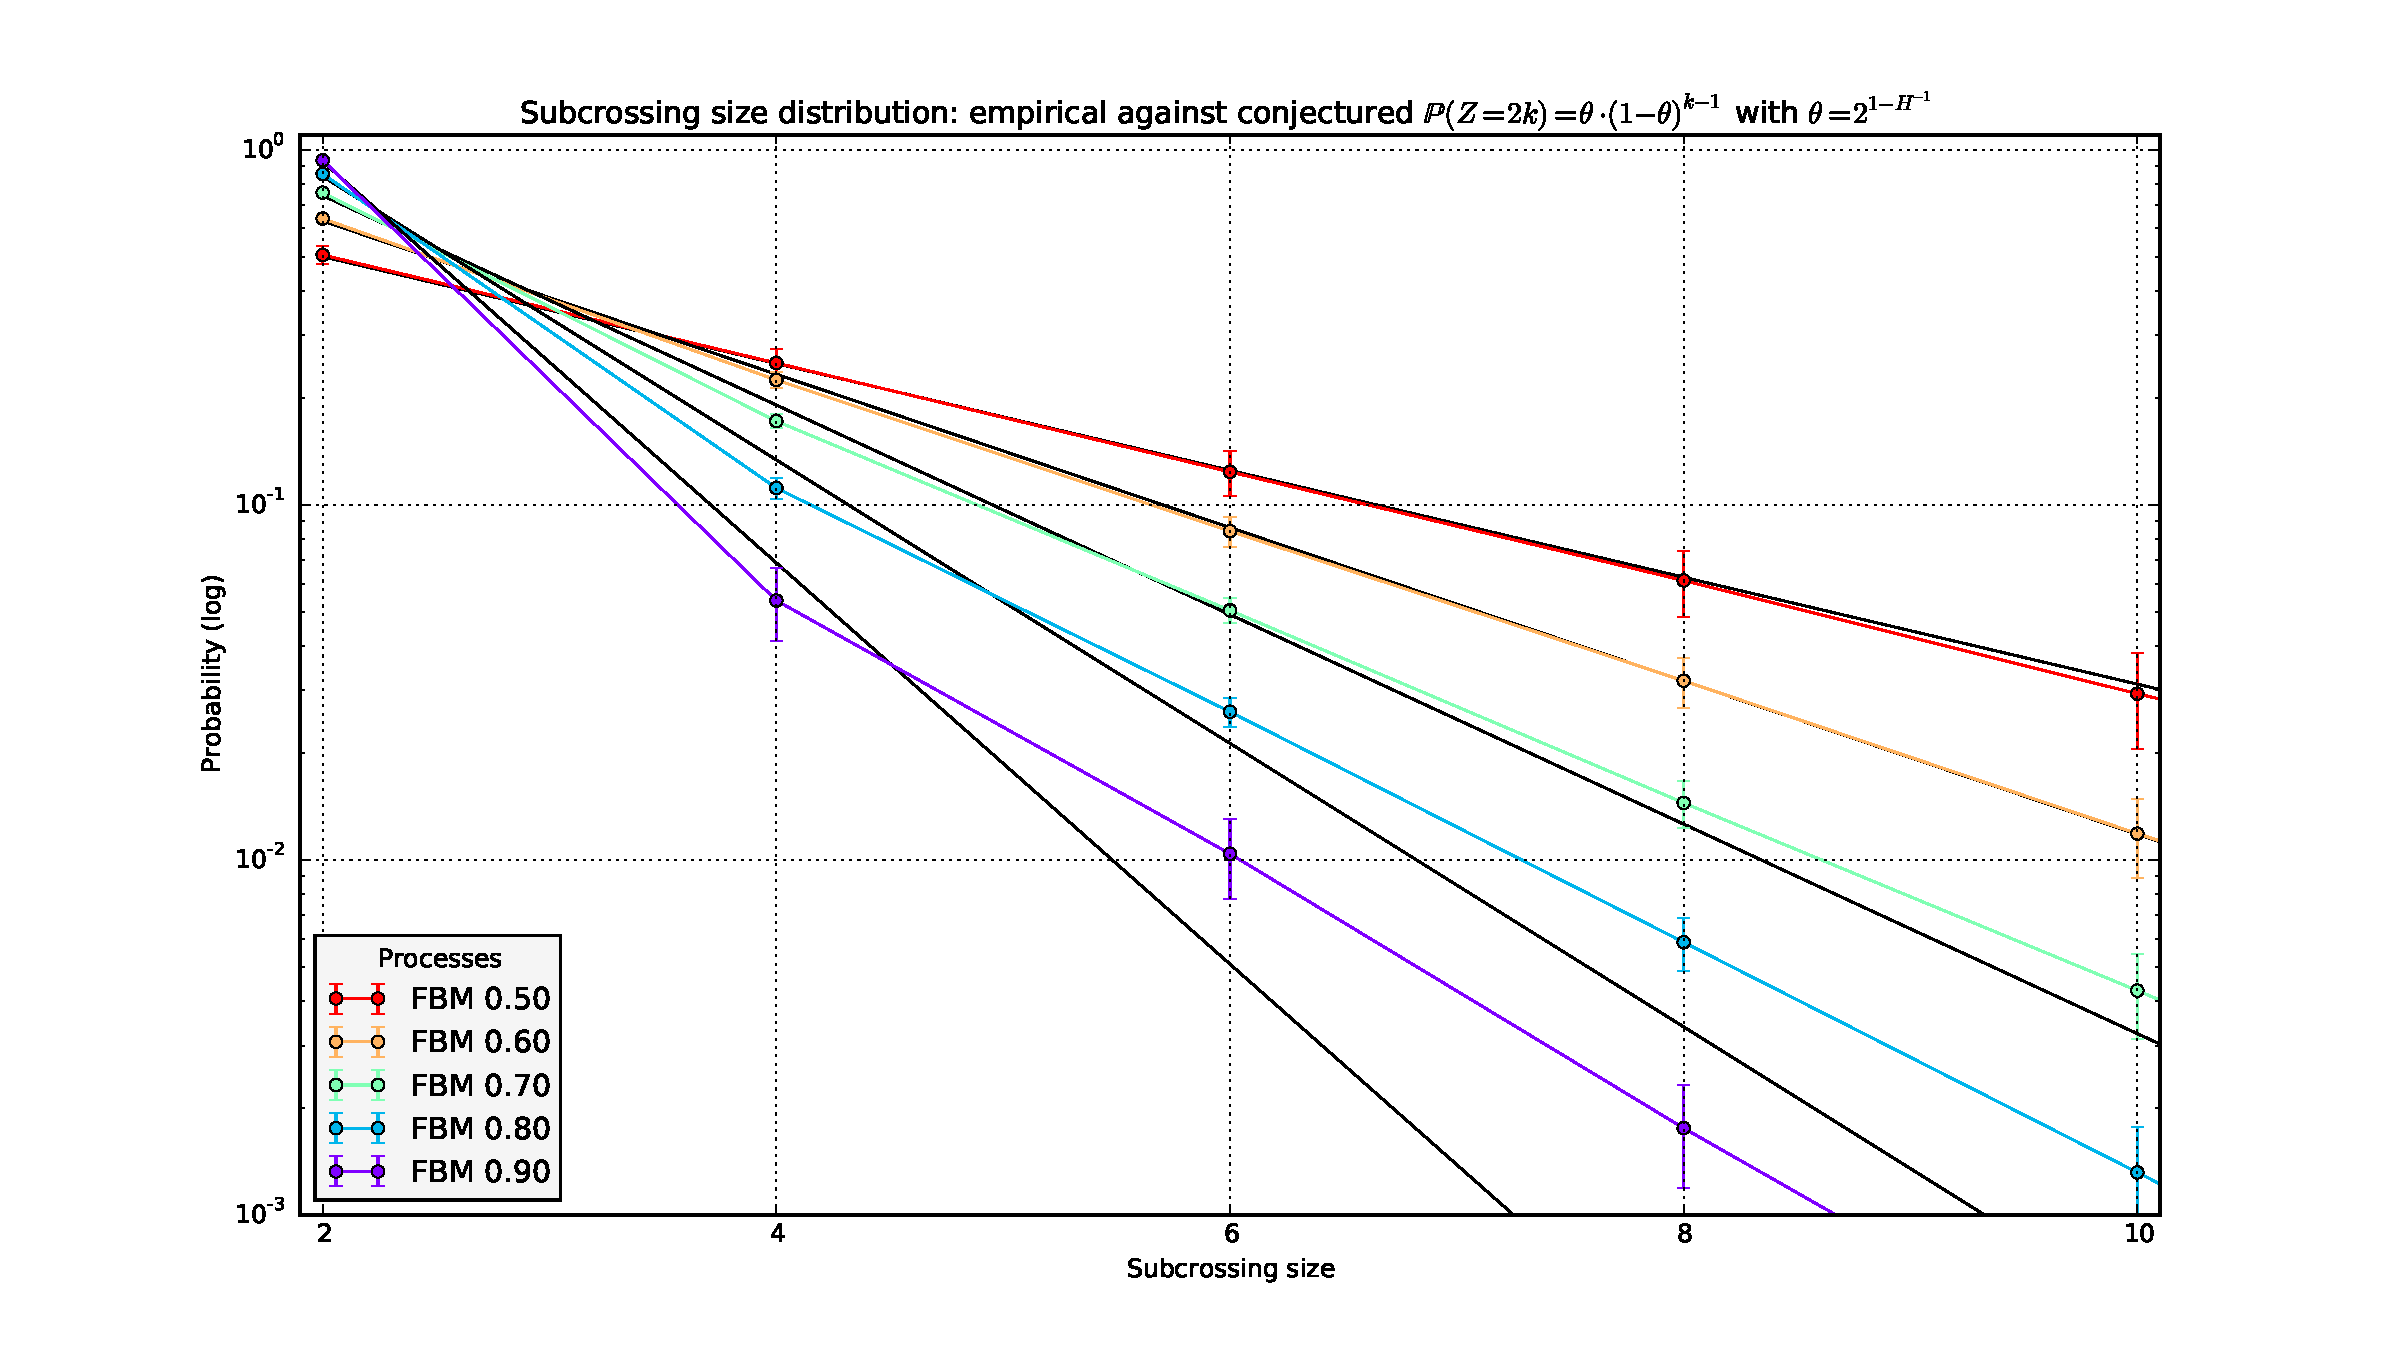
\includegraphics[draft,width=6in]{images/fbm_fig_01_med_1000-21}
    \caption{The log-plot of the offspring distributions estimated on 1000 sample discrete paths
    of the fBM process of length $2^{21}$ and Hurst exponents in the range from $0.5$ to $0.9$.}
\label{fig:fbm_offspring_distribution}
\end{center}\end{figure}
Similarly, the theoretical probability of an up-down crossing conditional on an upcrossing
is matched very closely by the numerical evidence (fig.~\ref{fig:fbm_offspring_up_down}).
The results are similar in the down-up excursions case (fig.~\ref{fig:fbm_offspring_down_up}).

\begin{figure}[htb]\begin{center}
    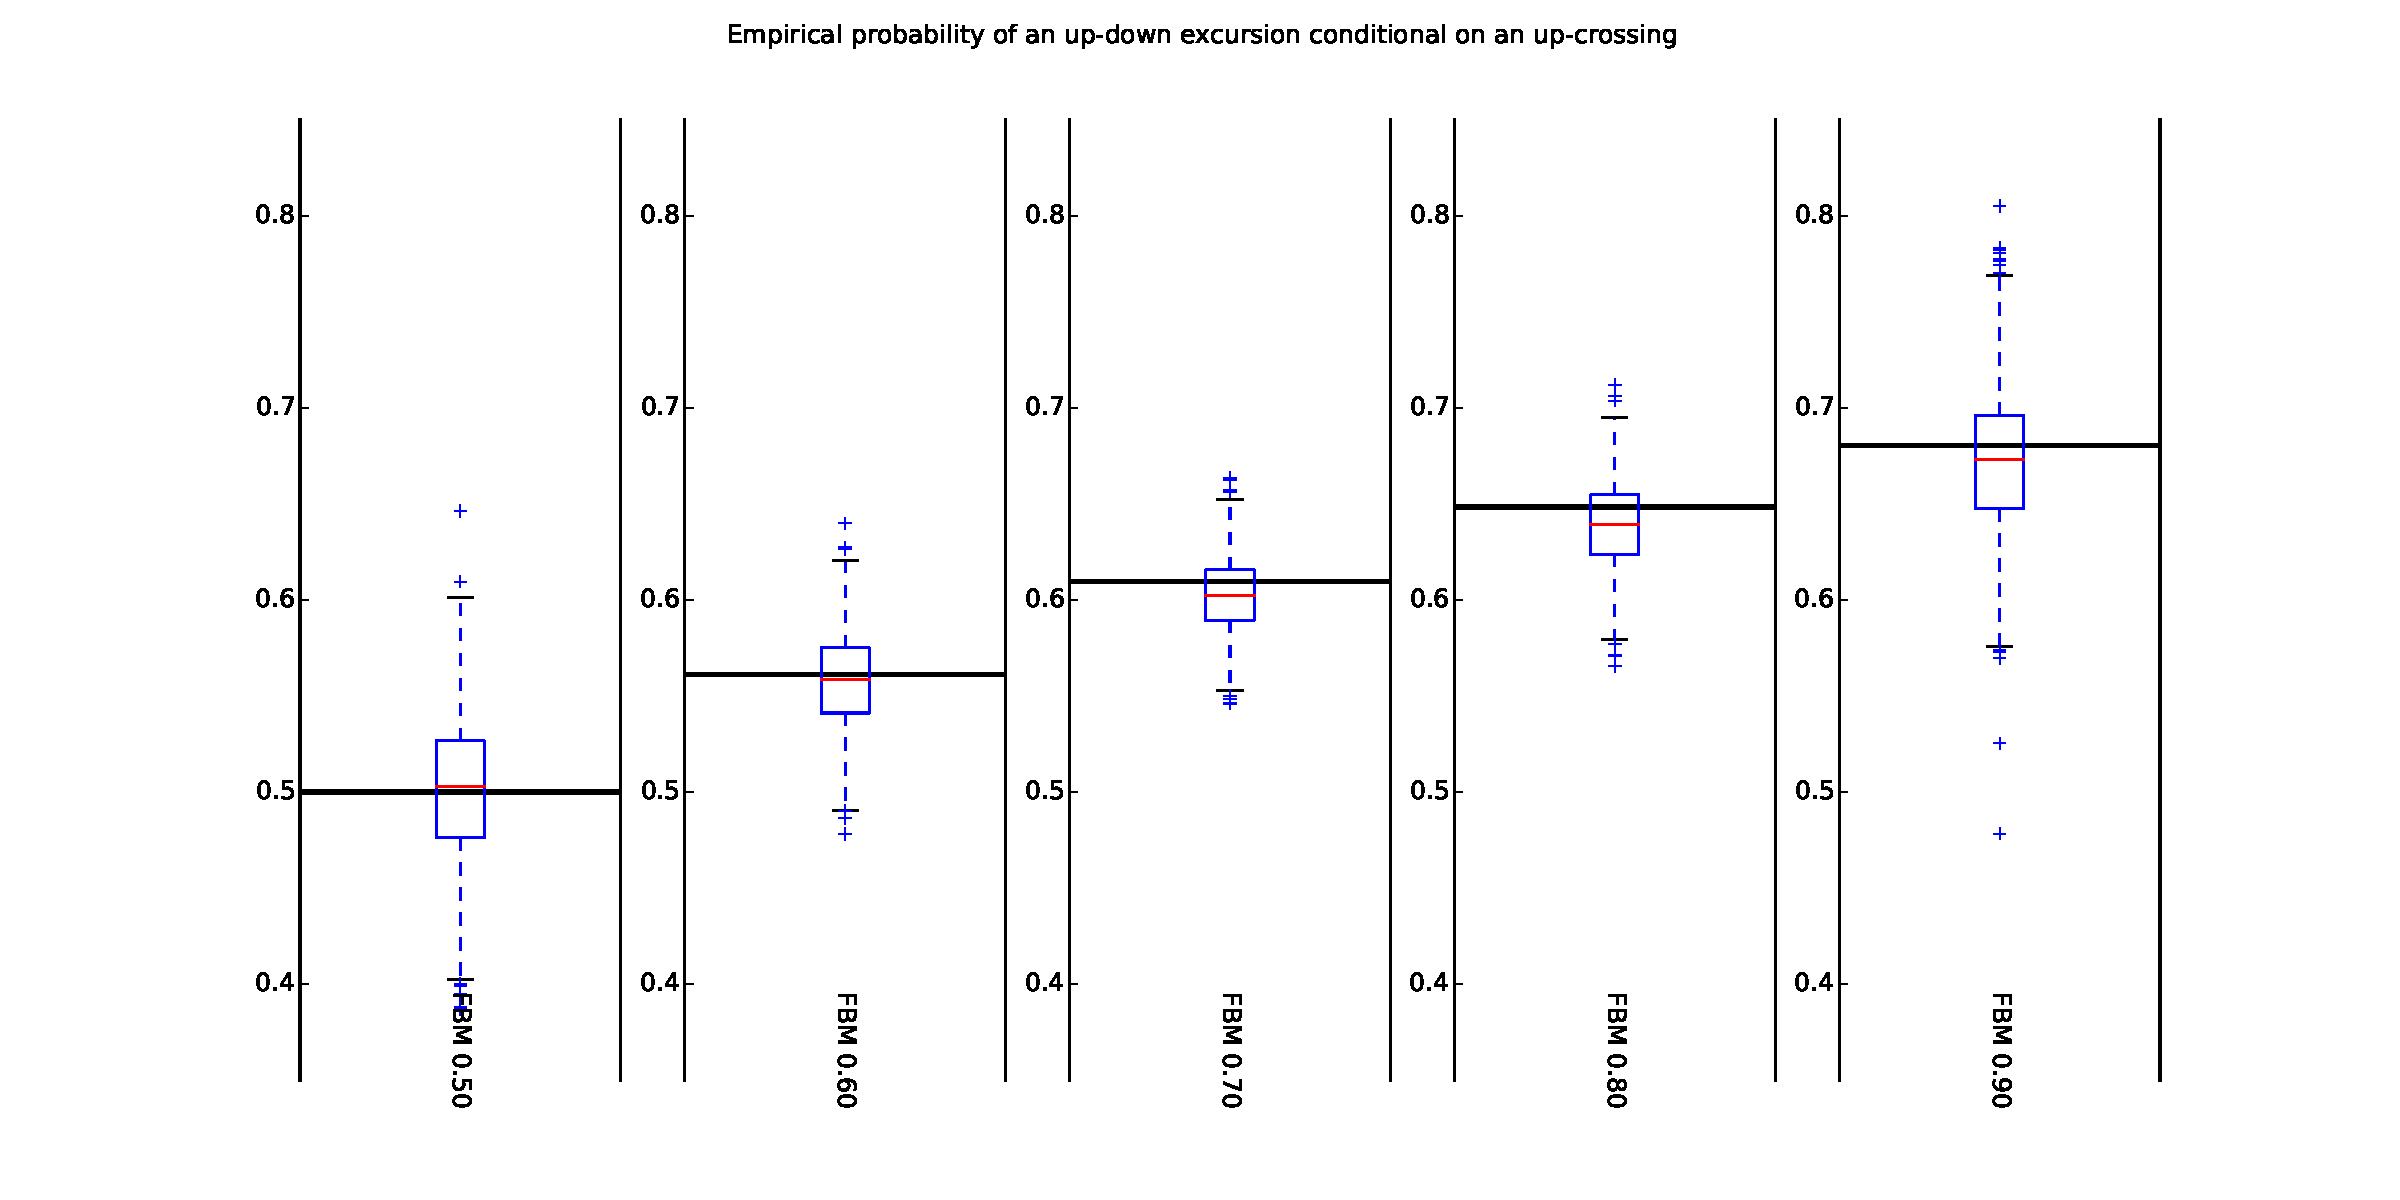
\includegraphics[draft,width=6in]{images/fbm_fig_03_up-down_med_1000-21}
    \caption{The estimated conditional probability of an up-down excursion given upward
    orientation of the parent crossing.}
\label{fig:fbm_offspring_up_down}
\end{center}\end{figure}

\begin{figure}[htb]\begin{center}
    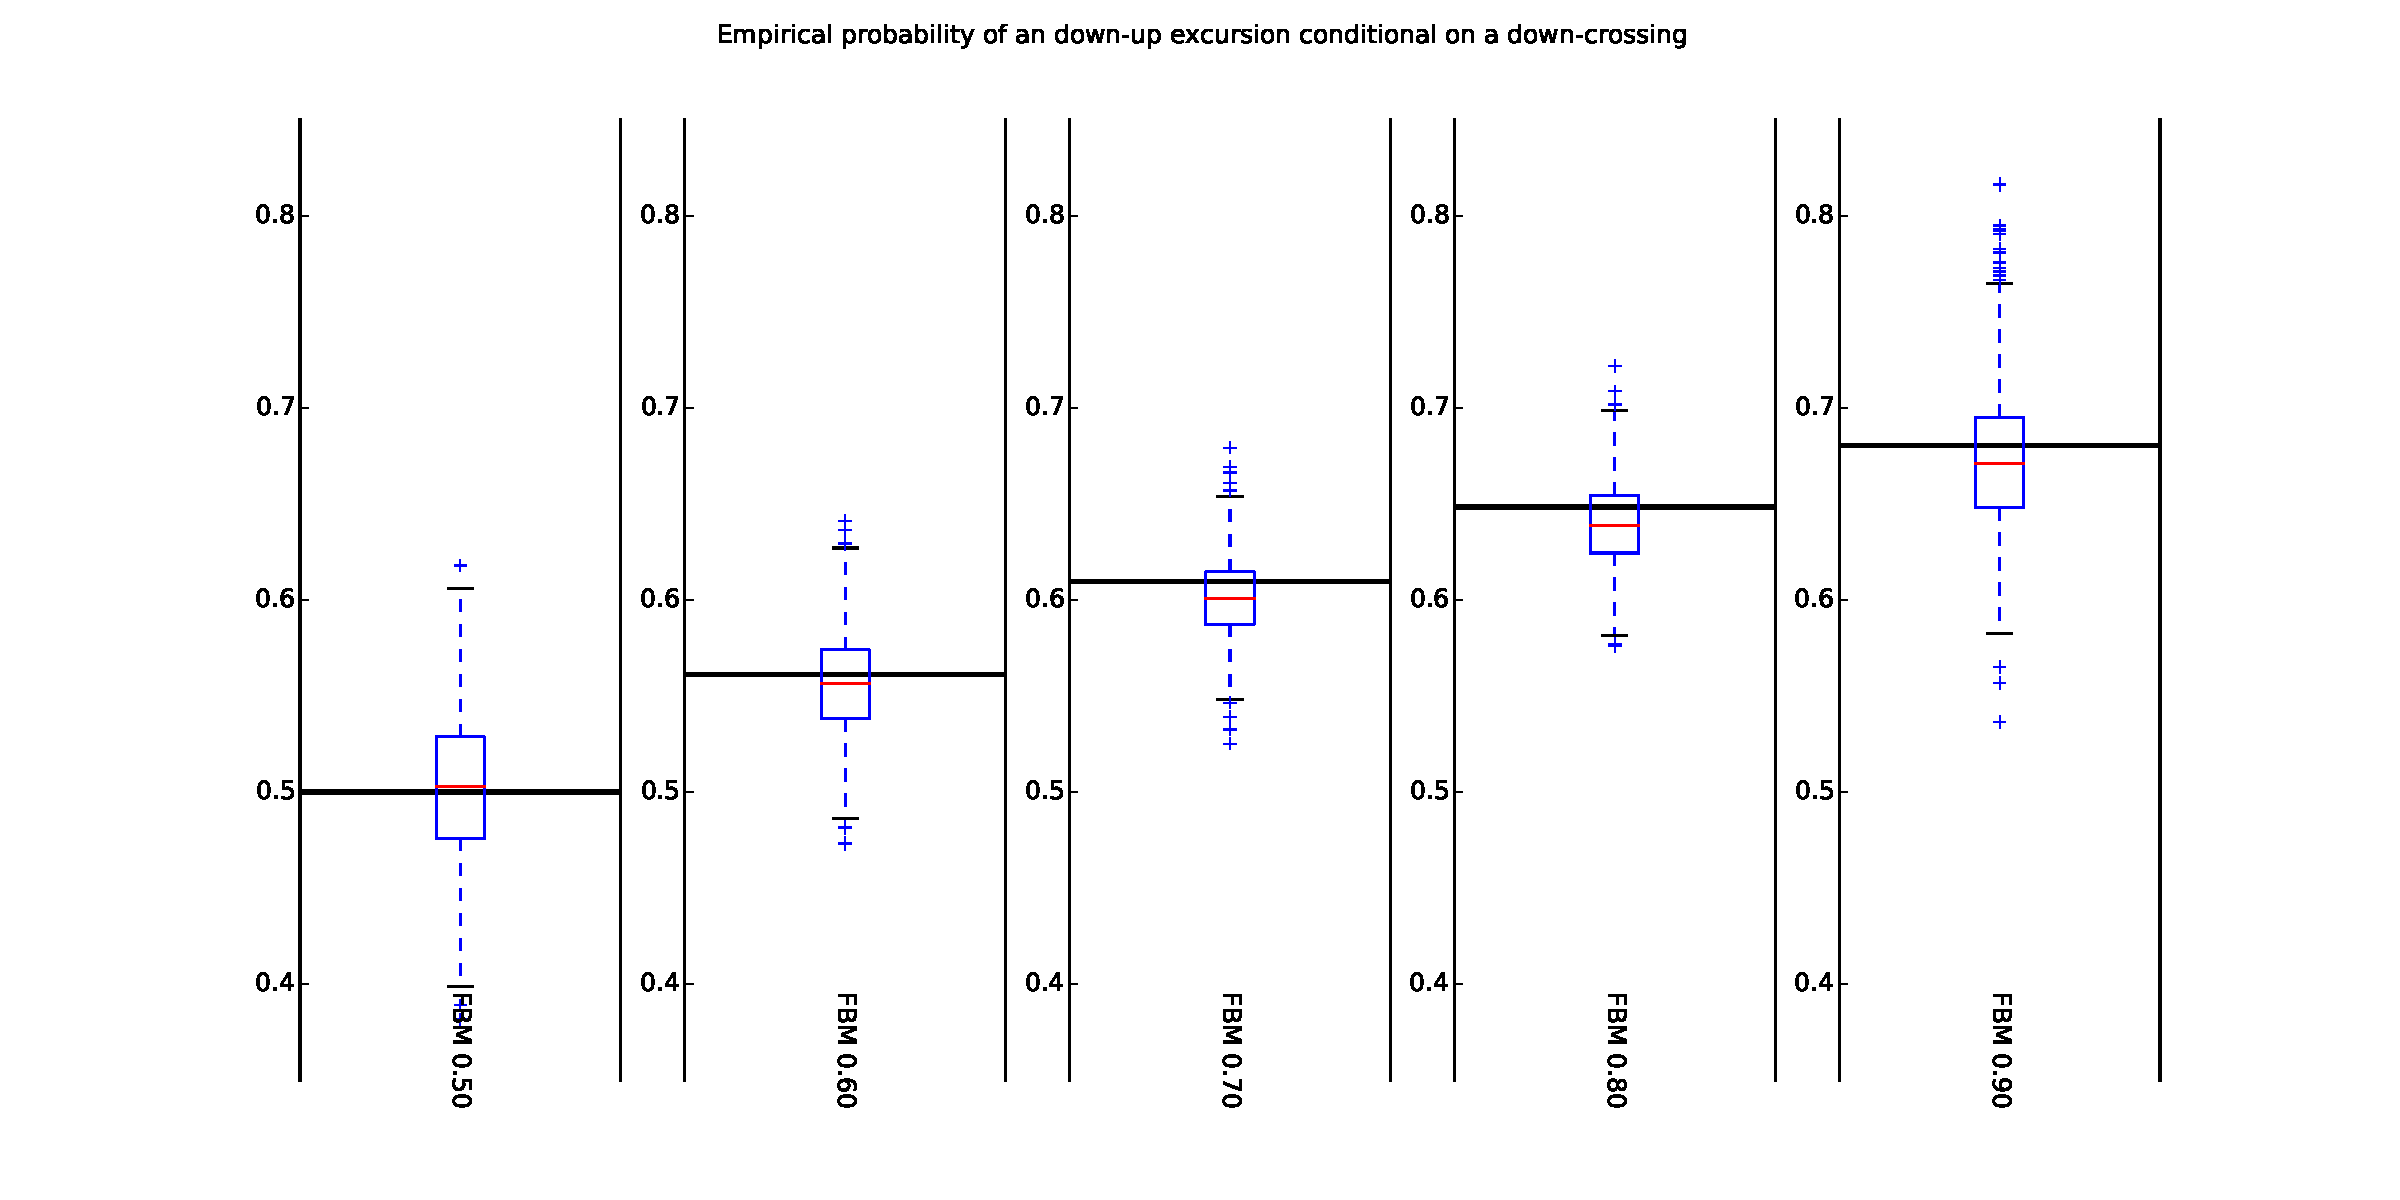
\includegraphics[draft,width=6in]{images/fbm_fig_03_down-up_med_1000-21}
    \caption{The box-plot of the estimates of the probability of an down-up excursion
    conditional on the orientation of the parent crossing being downward.}
\label{fig:fbm_offspring_down_up}
\end{center}\end{figure}

As for the conjectured distribution, the offspring distribution in the performed
experiments seems to suggest that the levels of the tree, at least for the fractional
Brownian motion, tend to be populated by crossings with more than predicted number
of subcrossings (see tables~\ref{tbl:empirical_probs_01} for $H=0.6$
and~\ref{tbl:empirical_probs_02} for $H=0.8$). However the failure of the conjectured
crossing size distribution to match the empirical results closely, should not be
considered as a serious evidence against it in this case. Indeed, the empirical
offspring distribution for fBM with $H=0.5,0.6$ and $0.7$ is aligned quite well
with the conjecture, and since there is no theoretical reason as to why the
dependence on $H$ should break down for values of $H$ closer to $1$, we attribute
this discrepancy to numerical issues of discretizing continuous processes and
simulating fGn with long range dependence. 

Finally, the mean crossing durations, averaged for each replication across all detected
crossings of a single level indeed demonstrate plausibility of the conjectured scaling
between levels of the crossing tree, see fig.~\ref{fig:fbm_avg_crossing_durations} for fBM.
\begin{figure}[htb]\begin{center}
    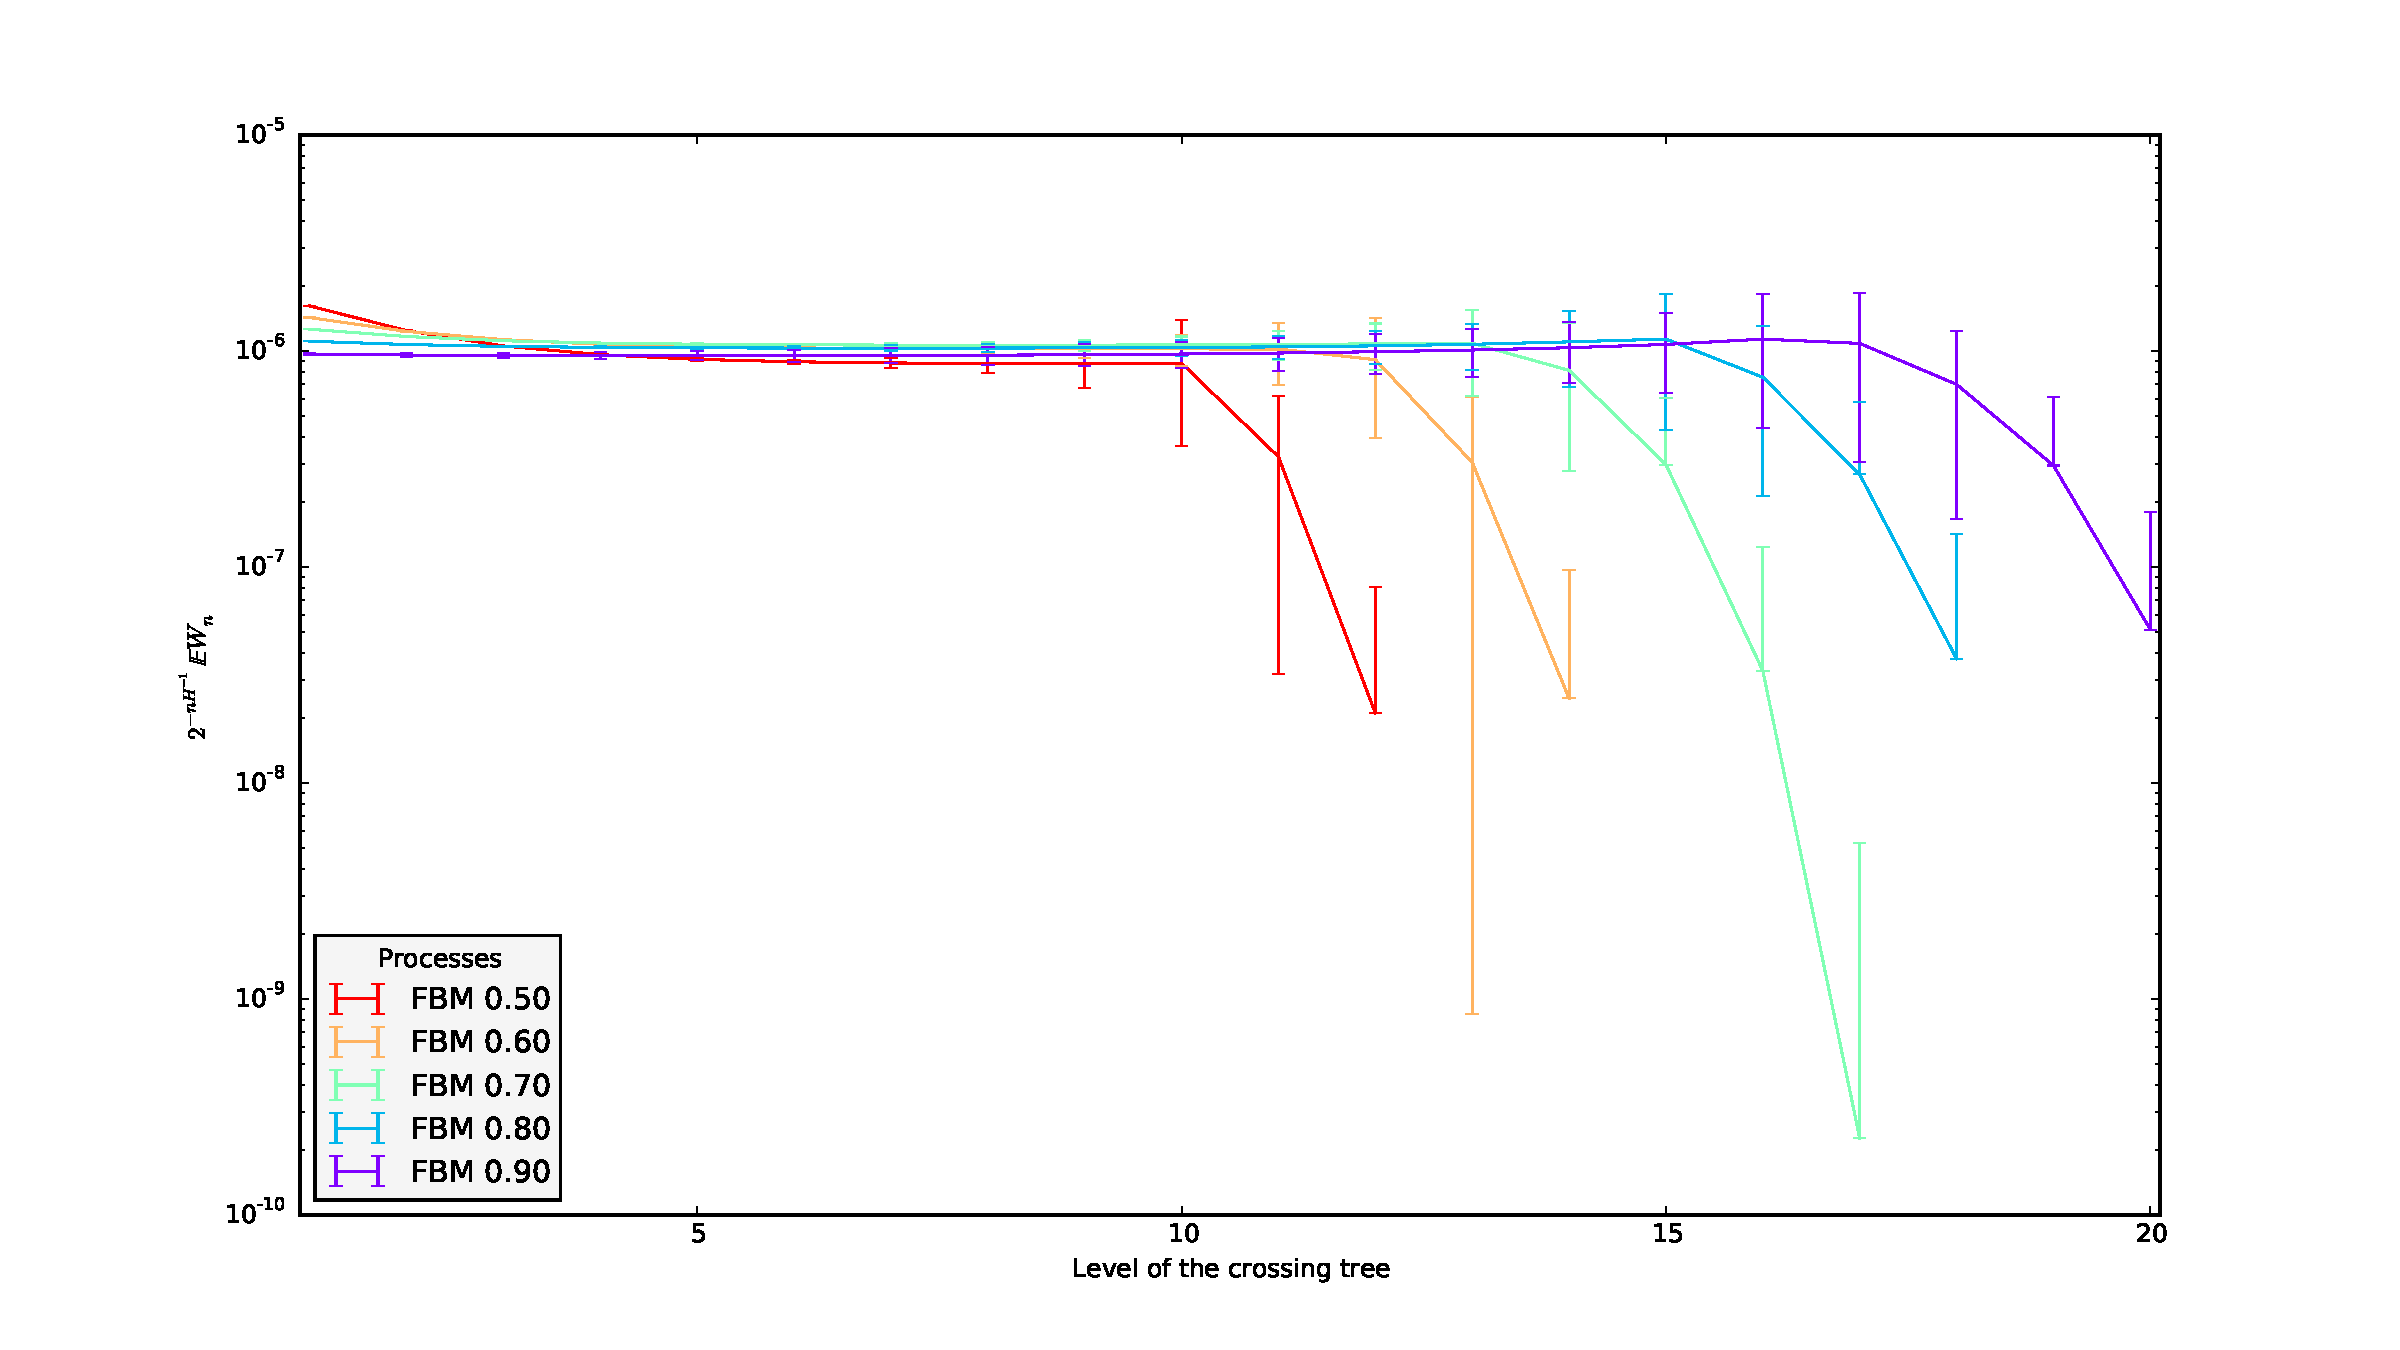
\includegraphics[draft,width=6in]{images/fbm_fig_08_med_1000-21}
    \caption{The average crossing duration at each level of the crossing tree built
    for fractional Brownian motion processes.}
\label{fig:fbm_avg_crossing_durations}
\end{center}\end{figure}

Now let's turn to the Hermite and Weierstrass processes. This time $10^4$ random
replications of sample paths of size $2^{17}$ were generated for each process.
This size limitation was dictated by deteriorating numerical accuracy of the procedure,
responsible for generating sample paths of Hermite processes. Thus in order to produce
comparable results, sample paths of fBM and Weierstrass processes were limited to $2^{17}$
points as well.

Figure~\ref{fig:all_hurst_crossing_tree} suggests that the processes studied share common
statistical properties of the crossing tree.
\begin{figure}[htb]\begin{center}
    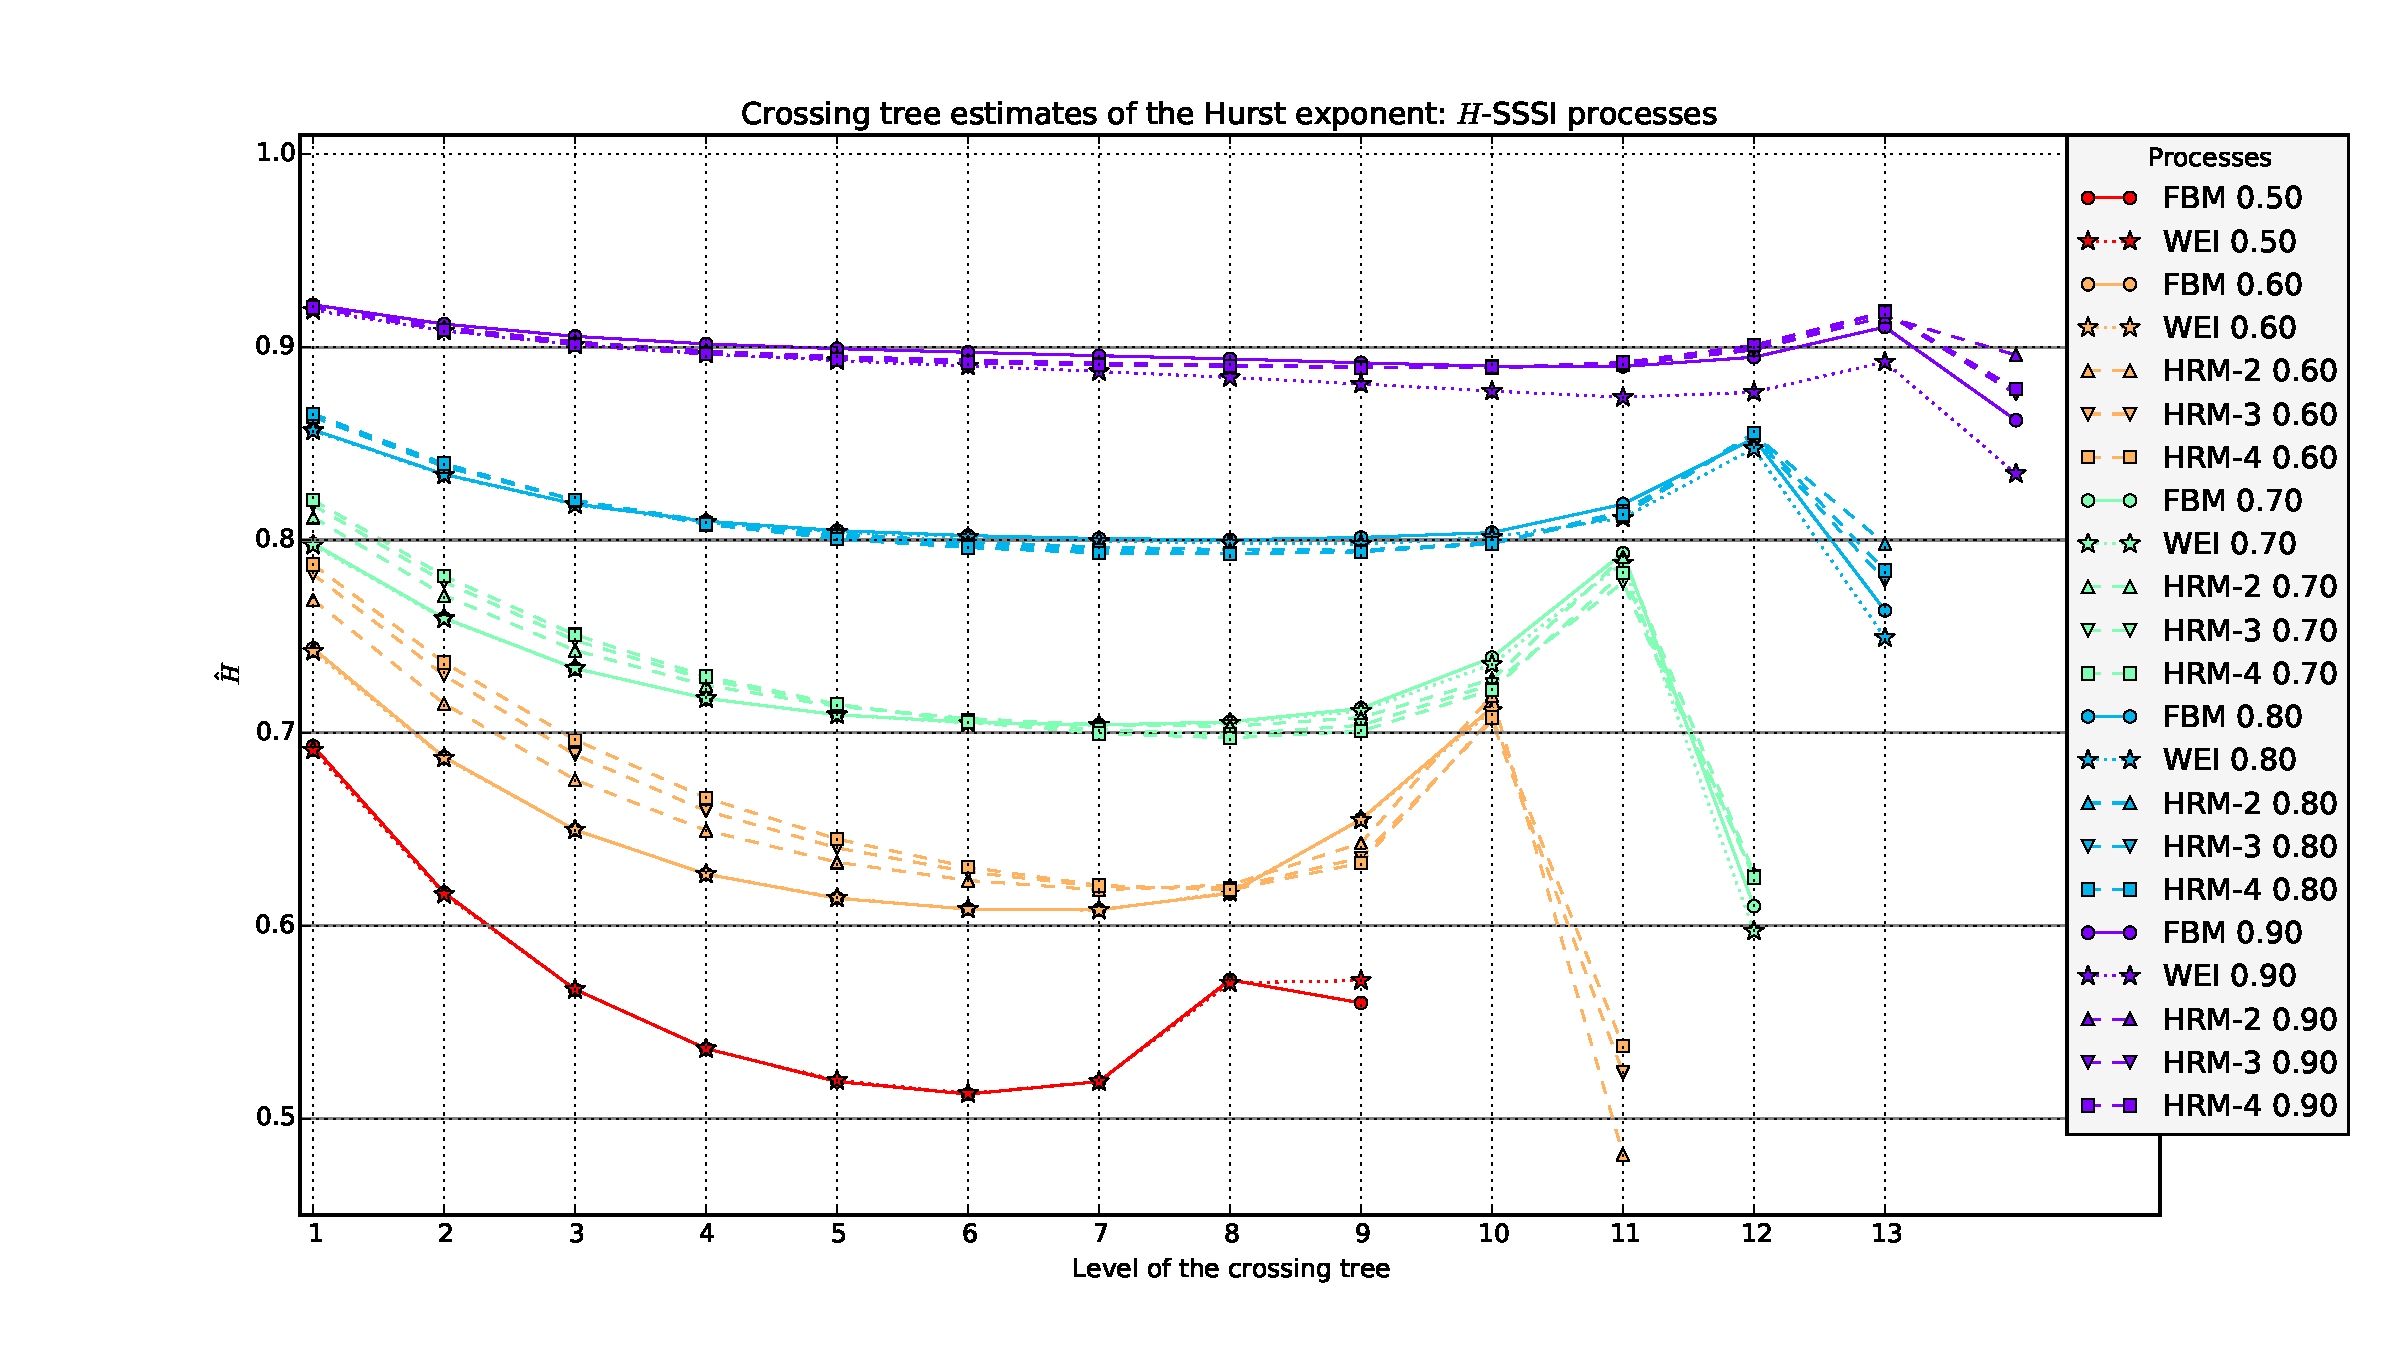
\includegraphics[draft,width=6in]{images/fig_05_med_10000-17}
    \caption{Estimates of the Hurst exponent $H$ based on a single level of the crossing tree for
    the all studied $H$-sssi processes.}
\label{fig:all_hurst_crossing_tree}
\end{center}\end{figure}

Table~\ref{tbl:chi_sq_test_for_all_01} summarizes the empirical rejection rates of
the $\chi^2$ test for self similarity across the range of levels indicated in the
header of the table.
\begin{table}[h]\begin{center}
	\begin{tabular}{l||c|c|c|c|c|c|}
	Process 		& $6-7$ &  $7-8$ &  $8-9$ &  $6-8$ &  $7-9$ &  $6-9$ \\ \hline\hline
	  fBM-$0.50$	& $9.7$ & $15.7$ &     -- & $13.8$ &  $\mathbf{3.6}$ &  $5.4$ \\ \hline
	  fBM-$0.60$	& $8.8$ &  $9.3$ &  $\mathbf{5.6}$ & $14.2$ & $14.3$ & $16.5$ \\ \hline
	  fBM-$0.70$	& $7.6$ &  $\mathbf{6.6}$ & $10.5$ & $13.4$ & $15.7$ & $17.8$ \\ \hline
	  fBM-$0.80$	& $6.5$ &  $4.8$ &  $\mathbf{4.5}$ & $11.5$ & $13.1$ & $16.5$ \\ \hline
	  fBM-$0.90$	& $\mathbf{4.5}$ &  $5.1$ &  $6.9$ & $11.7$ & $13.6$ & $19.8$ \\ \hline\hline

	  WEI-$0.50$	& $9.6$ & $12.4$ &     -- & $13.9$ &  $\mathbf{2.2}$ &  $5.1$ \\ \hline
	  WEI-$0.60$	& $\mathbf{8.2}$ &  $9.6$ & $11.1$ & $13.2$ & $14.8$ & $15.5$ \\ \hline
	  WEI-$0.70$	& $7.0$ &  $\mathbf{5.9}$ &  $\mathbf{5.9}$ & $12.9$ & $14.6$ & $15.8$ \\ \hline
	  WEI-$0.80$	& $6.2$ &  $5.5$ &  $\mathbf{4.9}$ & $13.1$ & $13.2$ & $17.0$ \\ \hline
	  WEI-$0.90$	& $5.0$ &  $\mathbf{1.9}$ &  $8.7$ & $12.2$ &  $9.7$ & $21.0$ \\ \hline\hline

	HRM-2-$0.60$ 	& $9.6$ &  $9.2$ &  $\mathbf{7.1}$ & $15.2$ & $15.9$ & $19.6$ \\ \hline
	HRM-2-$0.70$ 	& $8.5$ &  $\mathbf{7.4}$ & $11.3$ & $13.9$ & $15.1$ & $18.2$ \\ \hline
	HRM-2-$0.80$ 	& $6.5$ &  $\mathbf{5.4}$ &  $5.6$ & $12.5$ & $12.3$ & $17.8$ \\ \hline
	HRM-2-$0.90$ 	& $6.4$ &  $\mathbf{4.9}$ &  $0.0$ & $12.7$ & $14.5$ & $18.7$ \\ \hline\hline

	HRM-3-$0.60$ 	& $9.6$ &  $\mathbf{9.2}$ & $13.7$ & $15.6$ & $17.9$ & $20.3$ \\ \hline
	HRM-3-$0.70$ 	& $\mathbf{7.9}$ &  $8.1$ &  $\mathbf{7.9}$ & $14.5$ & $16.4$ & $19.2$ \\ \hline
	HRM-3-$0.80$ 	& $5.5$ &  $\mathbf{4.3}$ &  $5.4$ & $11.8$ & $13.1$ & $16.7$ \\ \hline
	HRM-3-$0.90$ 	& $\mathbf{5.6}$ &  $7.7$ & $12.5$ & $13.4$ & $14.1$ & $19.8$ \\ \hline\hline

	HRM-4-$0.60$ 	& $9.7$ &  $\mathbf{9.3}$ & $12.3$ & $16.5$ & $17.4$ & $21.4$ \\ \hline
	HRM-4-$0.70$ 	& $8.1$ &  $7.2$ &  $\mathbf{6.0}$ & $15.4$ & $16.8$ & $20.4$ \\ \hline
	HRM-4-$0.80$ 	& $5.7$ &  $7.4$ &  $\mathbf{1.8}$ & $11.7$ & $13.7$ & $16.8$ \\ \hline
	HRM-4-$0.90$ 	& $5.1$ &  $\mathbf{2.9}$ &  $8.3$ &  $9.8$ & $12.9$ & $19.0$ \\ \hline\hline

 	\end{tabular}
	\caption{The table of empirical rejection rate at significance level of $\alpha = 5\%$
	of the $\chi^2$ test for self-similarity between levels of the crossing tree. }
\label{tbl:chi_sq_test_for_all_01}
\end{center}\end{table}
There does not seem to be a common range of levels, at the corresponding resolutions of which
all processes exhibit scale invariance. This might be attributed to the fact that the path
of the generated processes were insufficiently long to adequately populate the higher
levels of the crossing tree. Nevertheless, it seems reasonable to expect a certain degree
of self-similarity over levels from 7 to 8, which with due caution, could yield empirical
evidence useful for analysing the conjecture.

Indeed, the offspring distribution plot (fig.~\ref{fig:all_xing_probs}) seems to
suggest that even though the theoretical distribution seems to underestimate the real
probability of a crossing of a particular size (in the number of subcrossings) as $H$
increases to $1$, there is still evidence for similarity of the statistical properties
of the crossing tree across different self-similar processes.
\begin{figure}[htb]\begin{center}
    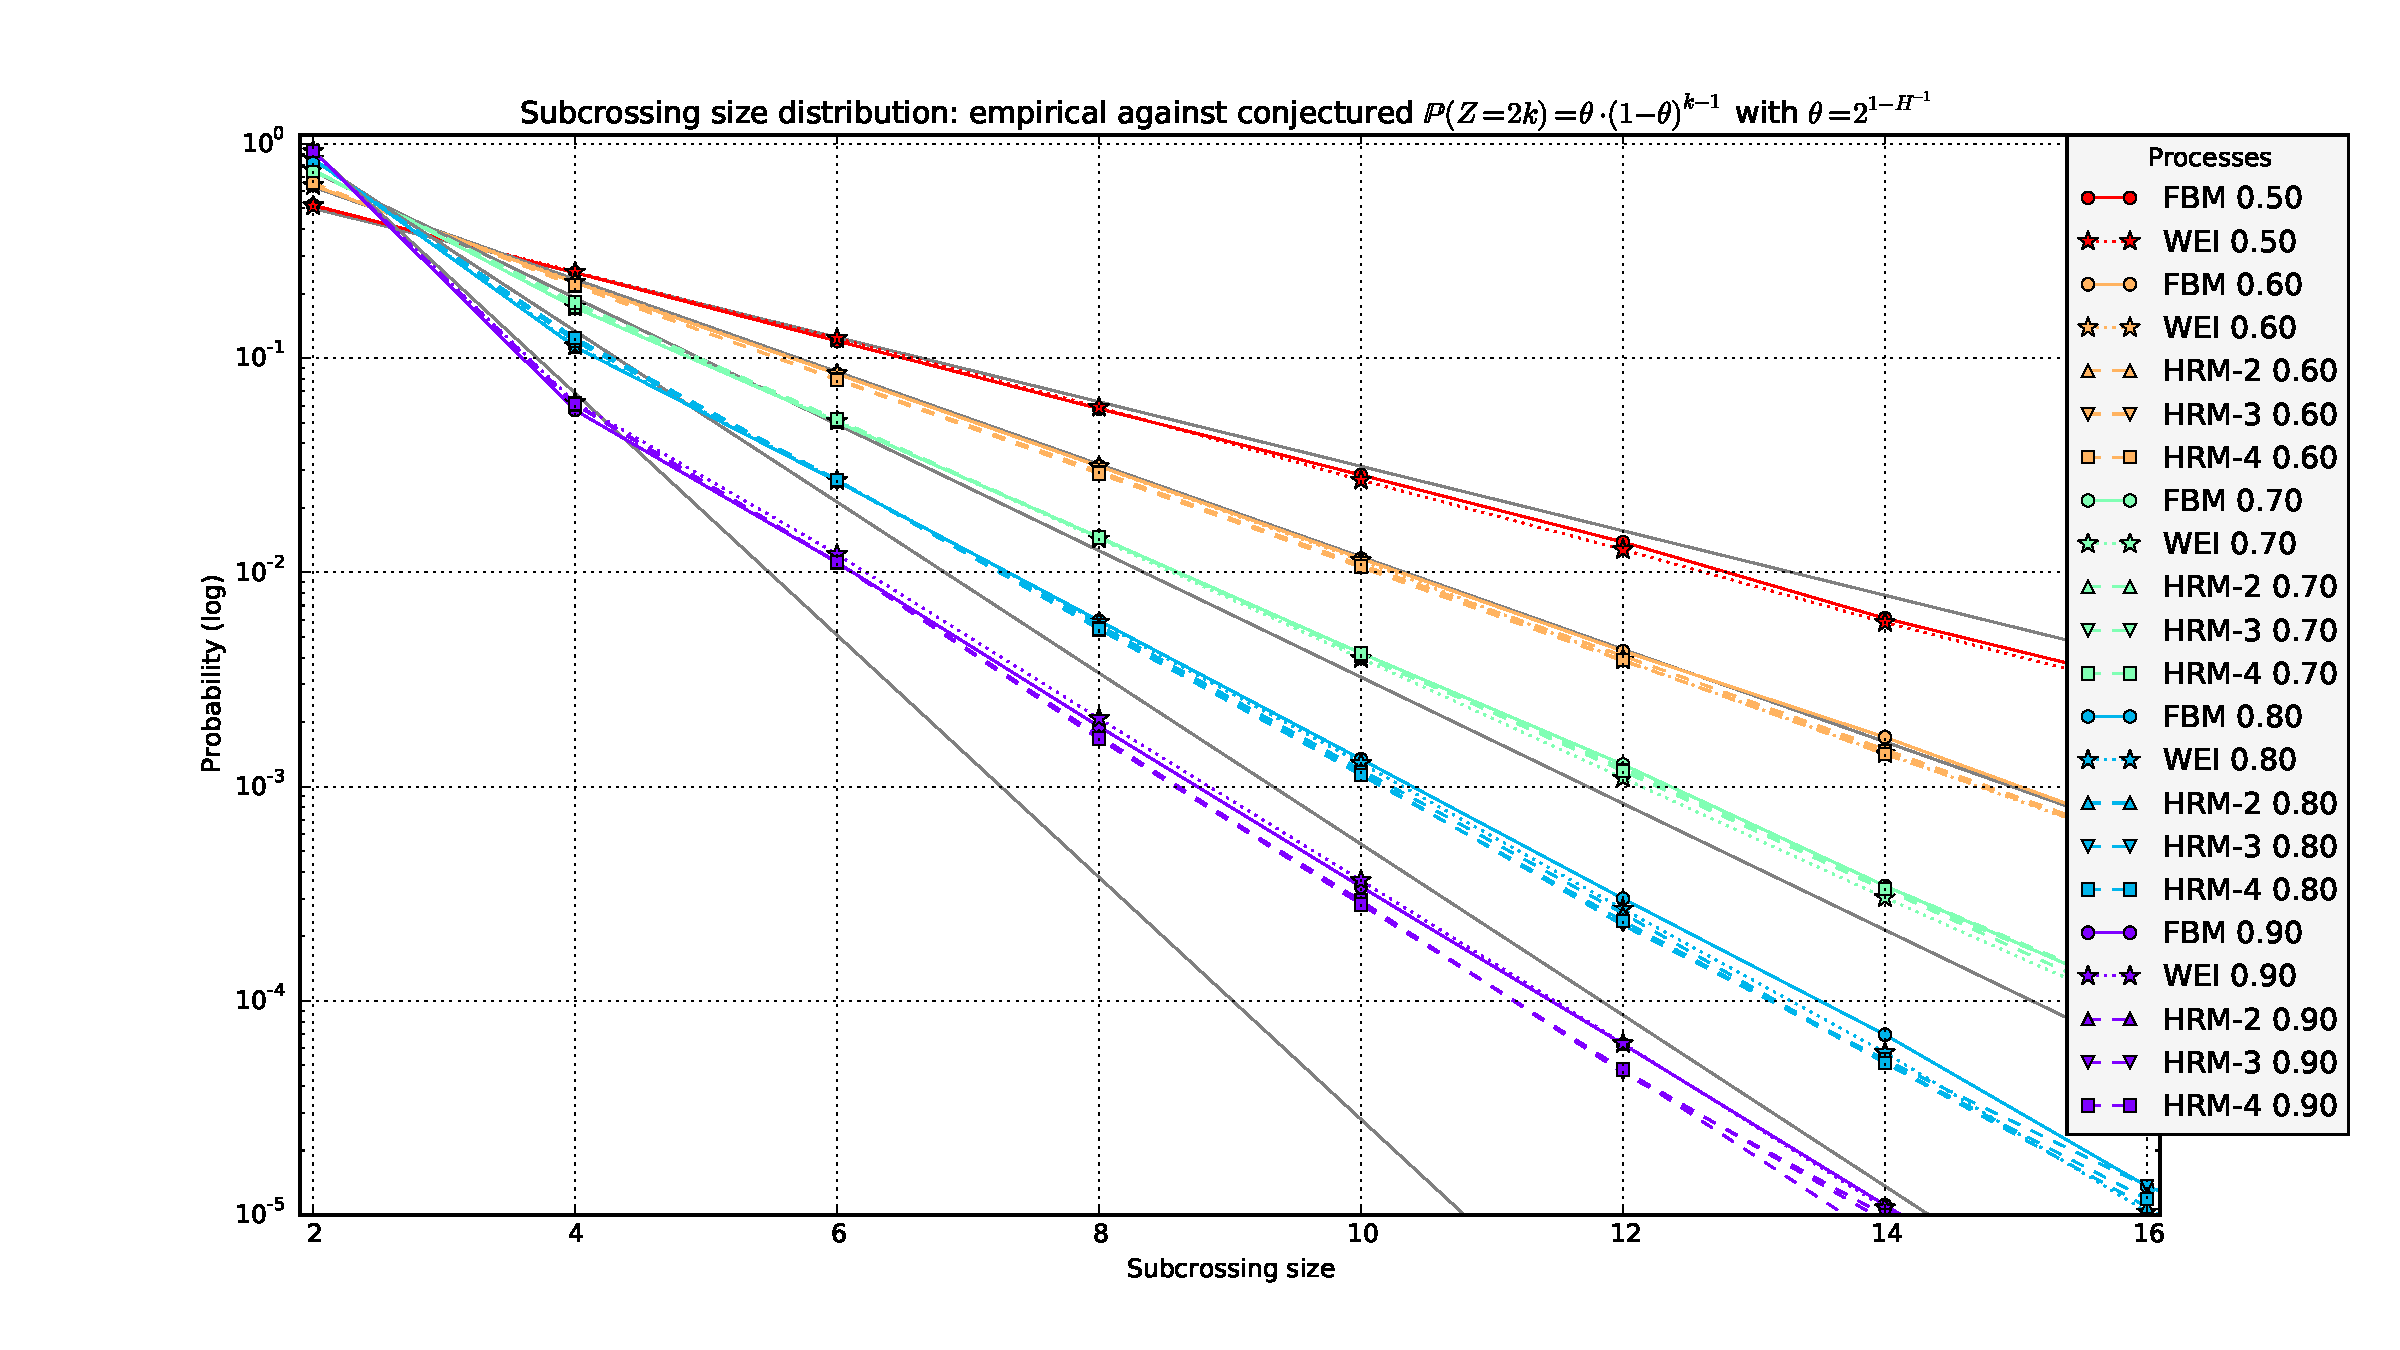
\includegraphics[draft,width=6in]{images/fig_02_med_10000-17}
    \caption{Empirical probabilities of the crossing sizes against the hypothesized
    theoretical probabilities for $10^4$ sample paths of length $2^{17}$ points.}
\label{fig:all_xing_probs}
\end{center}\end{figure}

The tables \ref{tbl:empirical_probs_01} and \ref{tbl:empirical_probs_02} compare the 
conjectured probabilities against the empirical ones. Though there is no strong evidence
for the conjecture, one cannot say that it should be discarded. Indeed, looking at
the box-plots (\ref{fig:all_offspring_down_up} and \ref{fig:all_offspring_up_down})
of the conditional distribution of excursions, it is possible to see that even
though there is significant margin of error there the probabilities seem to agree
quite well with the hypothesised distribution.
\begin{table}[h]\begin{center}
	\begin{tabular}{l||l|l|l|l|}
					$H=0.6$ & $Z_k = 2$ & $Z_k = 4$ & $Z_k = 6$ & $Z_k = 8$ \\ \hline\hline
	\multirow{2}{*}{fBM} 	& $0.630$ & $0.233$ & $0.086$ & $0.032$ \\ \cline{2-5}
							& $0.644\pm0.033$ & $0.224\pm0.027$ & $0.083\pm0.017$ & $0.031\pm0.011$ \\ \hline\hline
	\multirow{2}{*}{WEI} 	& $0.630$ & $0.233$ & $0.086$ & $0.032$ \\ \cline{2-5}
							& $0.642\pm0.027$ & $0.226\pm0.026$ & $0.084\pm0.017$ & $0.031\pm0.010$ \\ \hline\hline
	\multirow{2}{*}{HRM-2} 	& $0.630$ & $0.233$ & $0.086$ & $0.032$ \\ \cline{2-5}
							& $0.663\pm0.034$ & $0.215\pm0.026$ & $0.078\pm0.015$ & $0.028\pm0.009$ \\ \hline\hline
	\multirow{2}{*}{HRM-3} 	& $0.630$ & $0.233$ & $0.086$ & $0.032$ \\ \cline{2-5}
							& $0.666\pm0.038$ & $0.214\pm0.026$ & $0.076\pm0.015$ & $0.027\pm0.009$ \\ \hline\hline
	\multirow{2}{*}{HRM-4} 	& $0.630$ & $0.233$ & $0.086$ & $0.032$ \\ \cline{2-5}
							& $0.667\pm0.039$ & $0.215\pm0.025$ & $0.076\pm0.016$ & $0.027\pm0.009$ \\ \hline\hline
	\end{tabular}
	\caption{The table of empirical probabilities of the first four values of the number
	of subcrossings in a parent crossing for $H$-sssi processes with $H=0.6$. Levels from
	6 to 8 were pooled to get the estimates.}
\label{tbl:empirical_probs_01}
\end{center}\end{table}

\begin{table}[h]\begin{center}
	\begin{tabular}{l||l|l|l|l|}
					$H=0.8$ & $Z_k = 2$ & $Z_k = 4$ & $Z_k = 6$ & $Z_k = 8$ \\ \hline\hline
	\multirow{2}{*}{fBM} 	& $0.841$ & $0.134$ & $0.021$ & $0.003$ \\ \cline{2-5}
 							& $0.855\pm0.023$ & $0.112\pm0.017$ & $0.026\pm0.006$ & $0.006\pm0.002$ \\ \hline\hline
	\multirow{2}{*}{HRM-2} 	& $0.841$ & $0.134$ & $0.021$ & $0.003$ \\ \cline{2-5}
 							& $0.848\pm0.027$ & $0.118\pm0.022$ & $0.026\pm0.006$ & $0.005\pm0.002$ \\ \hline\hline
	\multirow{2}{*}{HRM-3} 	& $0.841$ & $0.134$ & $0.021$ & $0.003$ \\ \cline{2-5}
 							& $0.846\pm0.024$ & $0.121\pm0.019$ & $0.026\pm0.006$ & $0.005\pm0.002$ \\ \hline\hline
	\multirow{2}{*}{HRM-4} 	& $0.841$ & $0.134$ & $0.021$ & $0.003$ \\ \cline{2-5}
 							& $0.844\pm0.021$ & $0.122\pm0.016$ & $0.026\pm0.006$ & $0.005\pm0.002$ \\ \hline\hline
	\multirow{2}{*}{WEI} 	& $0.841$ & $0.134$ & $0.021$ & $0.003$ \\ \cline{2-5}
 							& $0.854\pm0.019$ & $0.113\pm0.015$ & $0.026\pm0.005$ & $0.006\pm0.002$ \\ \hline\hline
	\end{tabular}
	\caption{The table of empirical probabilities of the first four values of the number
	of subcrossings in a parent crossing for $H$-sssi processes with $H=0.8$. Levels from
	6 to 8 were pooled to get the estimates.}
\label{tbl:empirical_probs_02}
\end{center}\end{table}

Crossing duration also do not seem contradict the hypothesized scaling for $H$-sssi
processes and the Weierstrass function (see fig.~\ref{fig:wei_durations} - \ref{fig:hrm_4_durations}).
Also we considered the properly scaled empirical quantiles (not presented here) of
the crossing durations between the processes considered and across all sufficiently
populated levels (from $1$-st to $10$-th) of the sample crossing tree. The conclusion
is that there is indeed similarity (up to a multiplicative constant depending on
the base scale $\delta$) of the crossing durations' distribution among processes
(see fig.~\ref{fig:fbm_quantiles_06}, \ref{fig:fbm_quantiles_08} and \ref{fig:fbm_quantiles_durations}).

\begin{figure}[htb]\begin{center}
    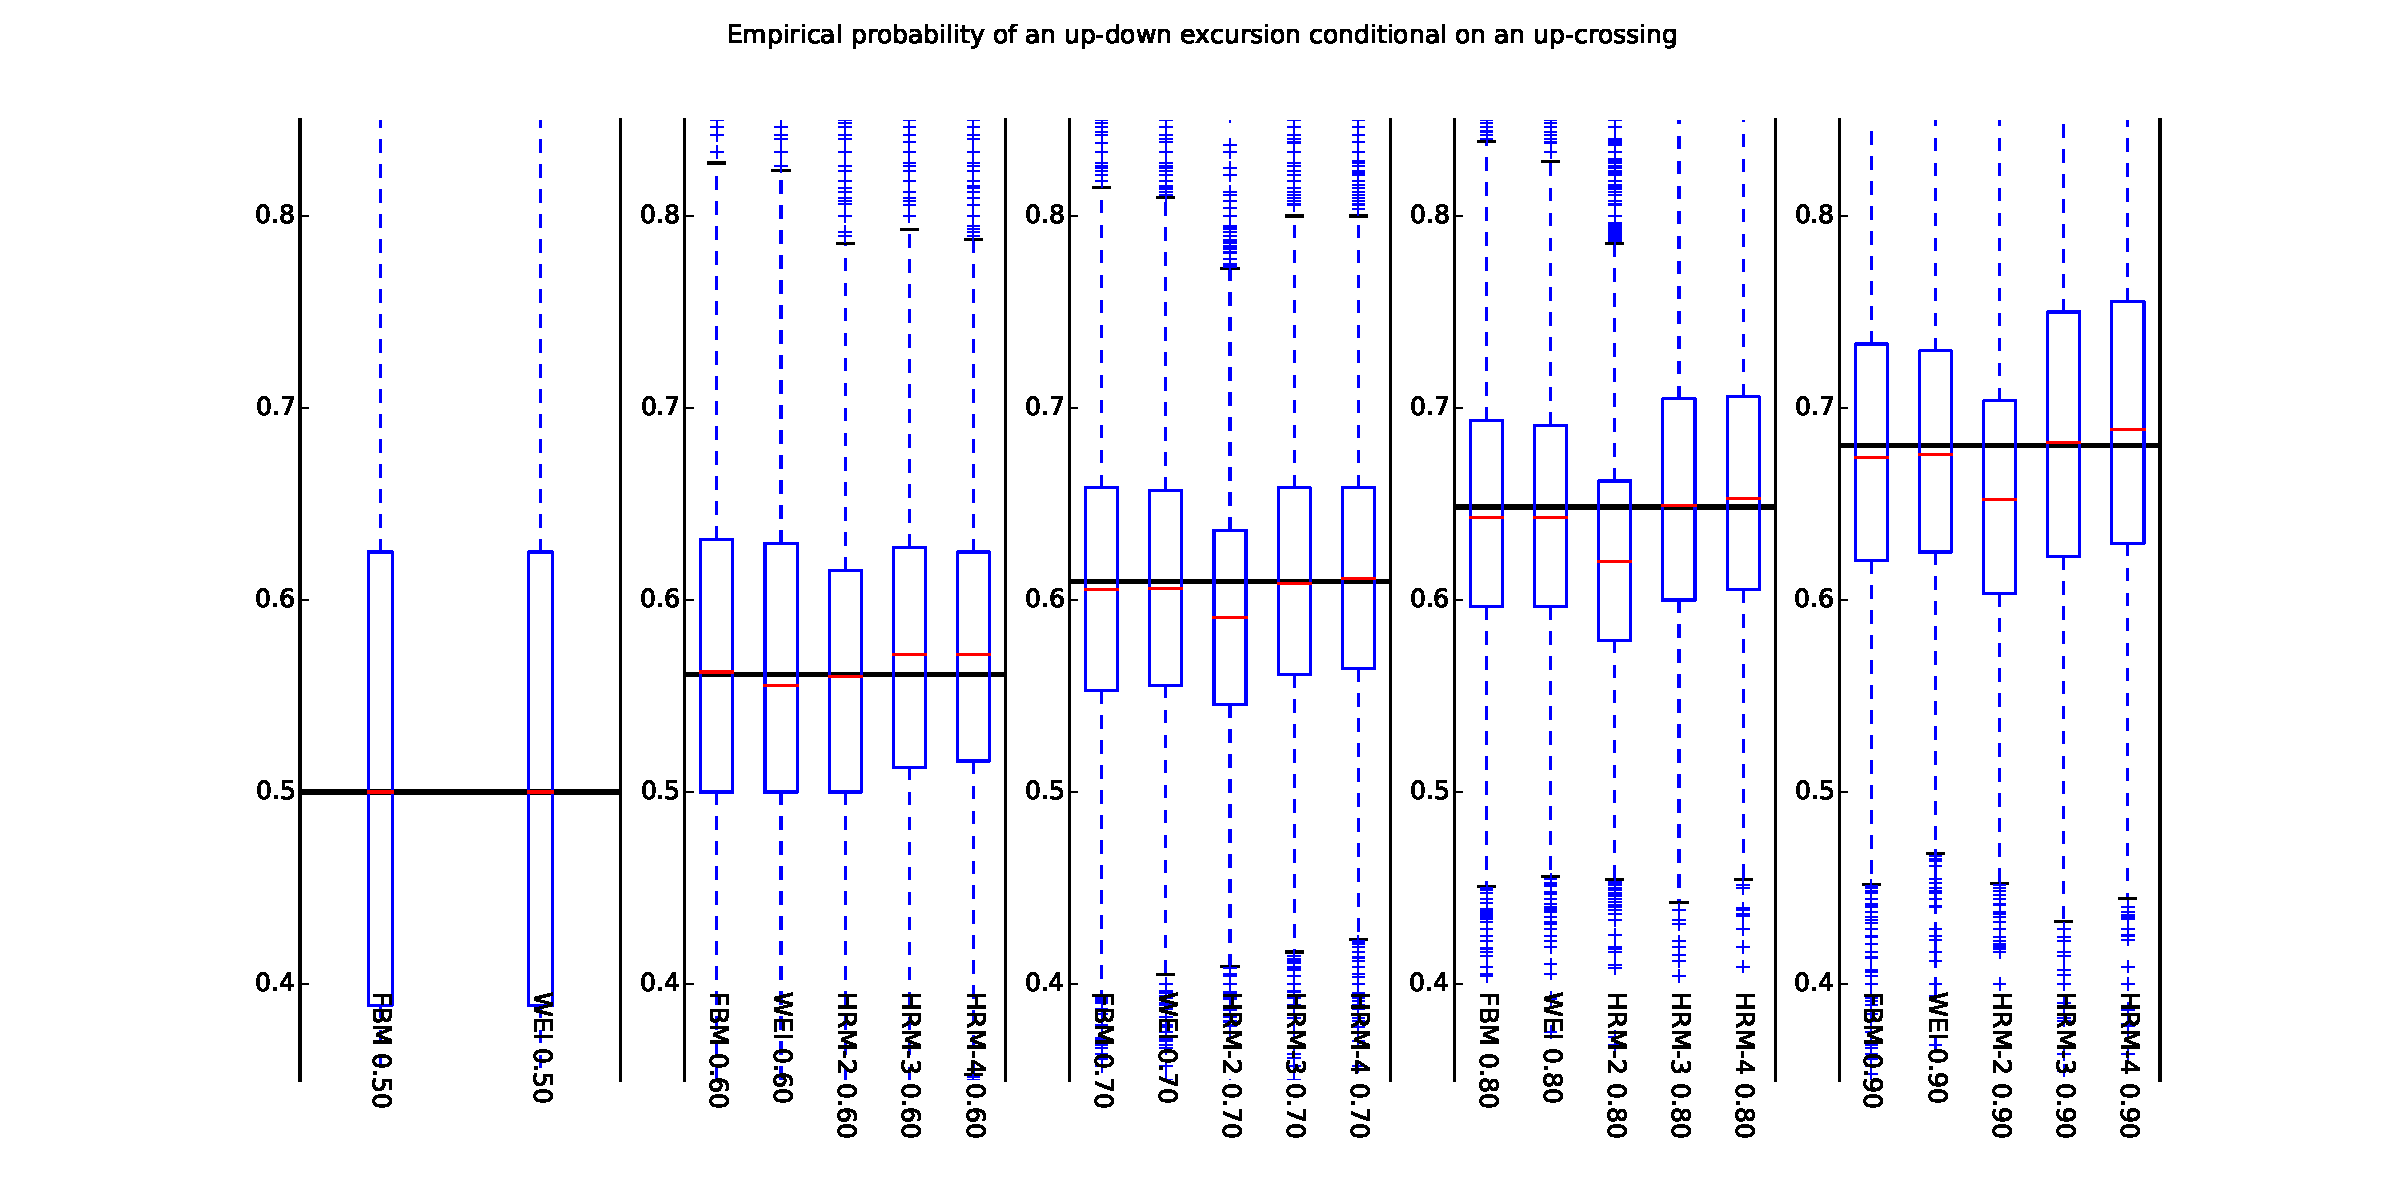
\includegraphics[draft,width=6in]{images/fig_03_up-down_med_10000-17}
    \caption{The empirical estimates of the probability of an up-down excursion conditional on
    the upward orientation of the parent crossing.}
\label{fig:all_offspring_up_down}
\end{center}\end{figure}

\begin{figure}[htb]\begin{center}
    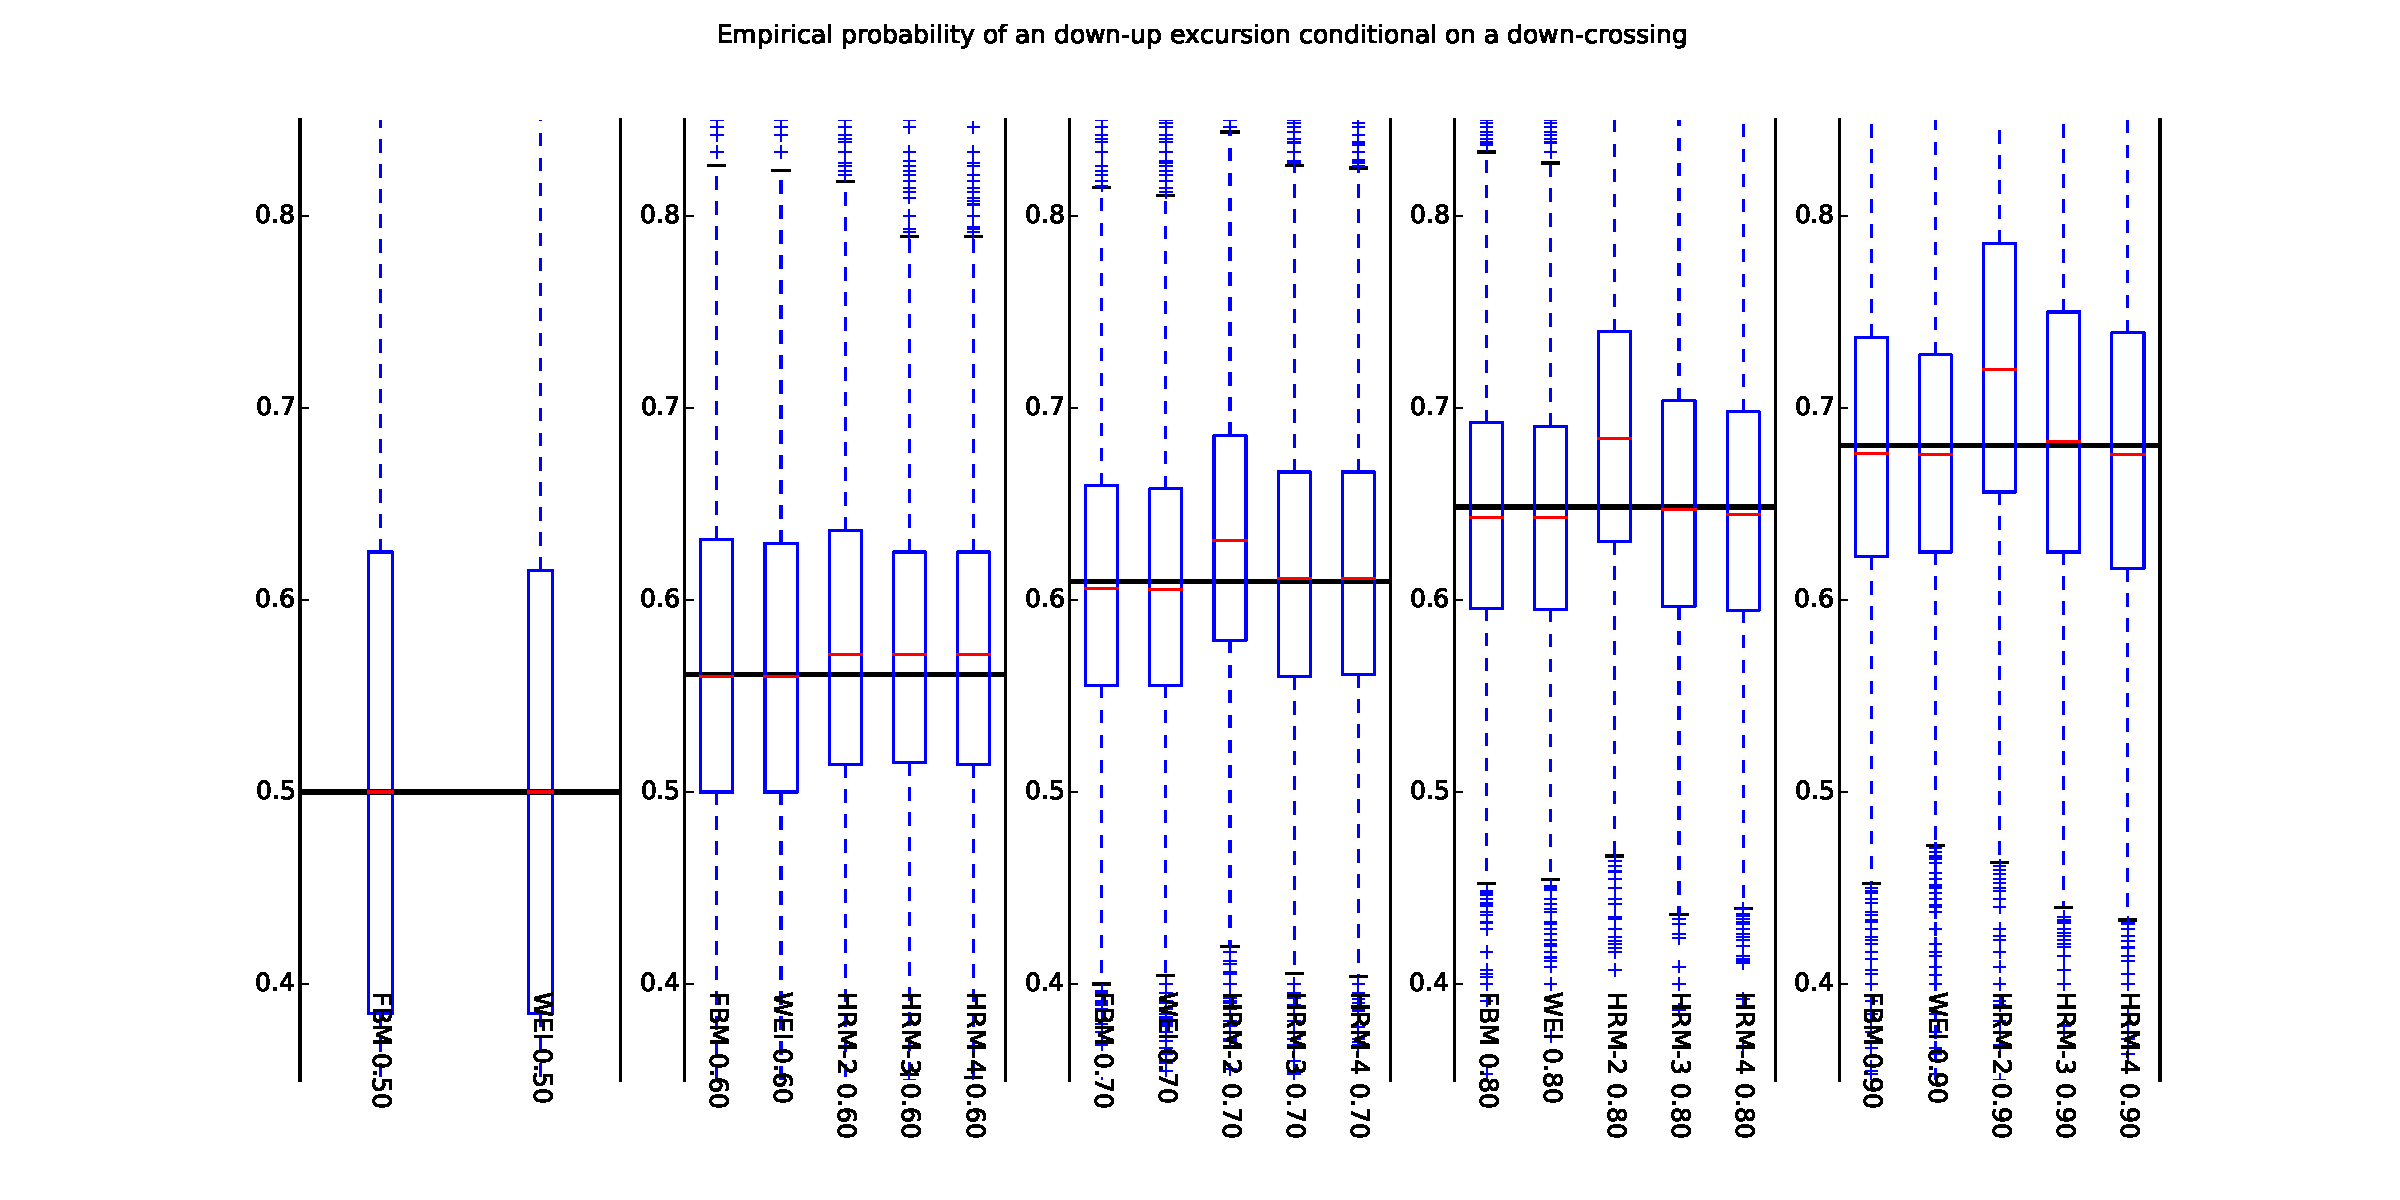
\includegraphics[draft,width=6in]{images/fig_03_down-up_med_10000-17}
    \caption{The same figure as~\ref{fig:all_offspring_up_down} but for down-up excursions
    conditional on the orientation of the parent crossing being downward.}
\label{fig:all_offspring_down_up}
\end{center}\end{figure}

\begin{figure}[htb]\begin{center}
    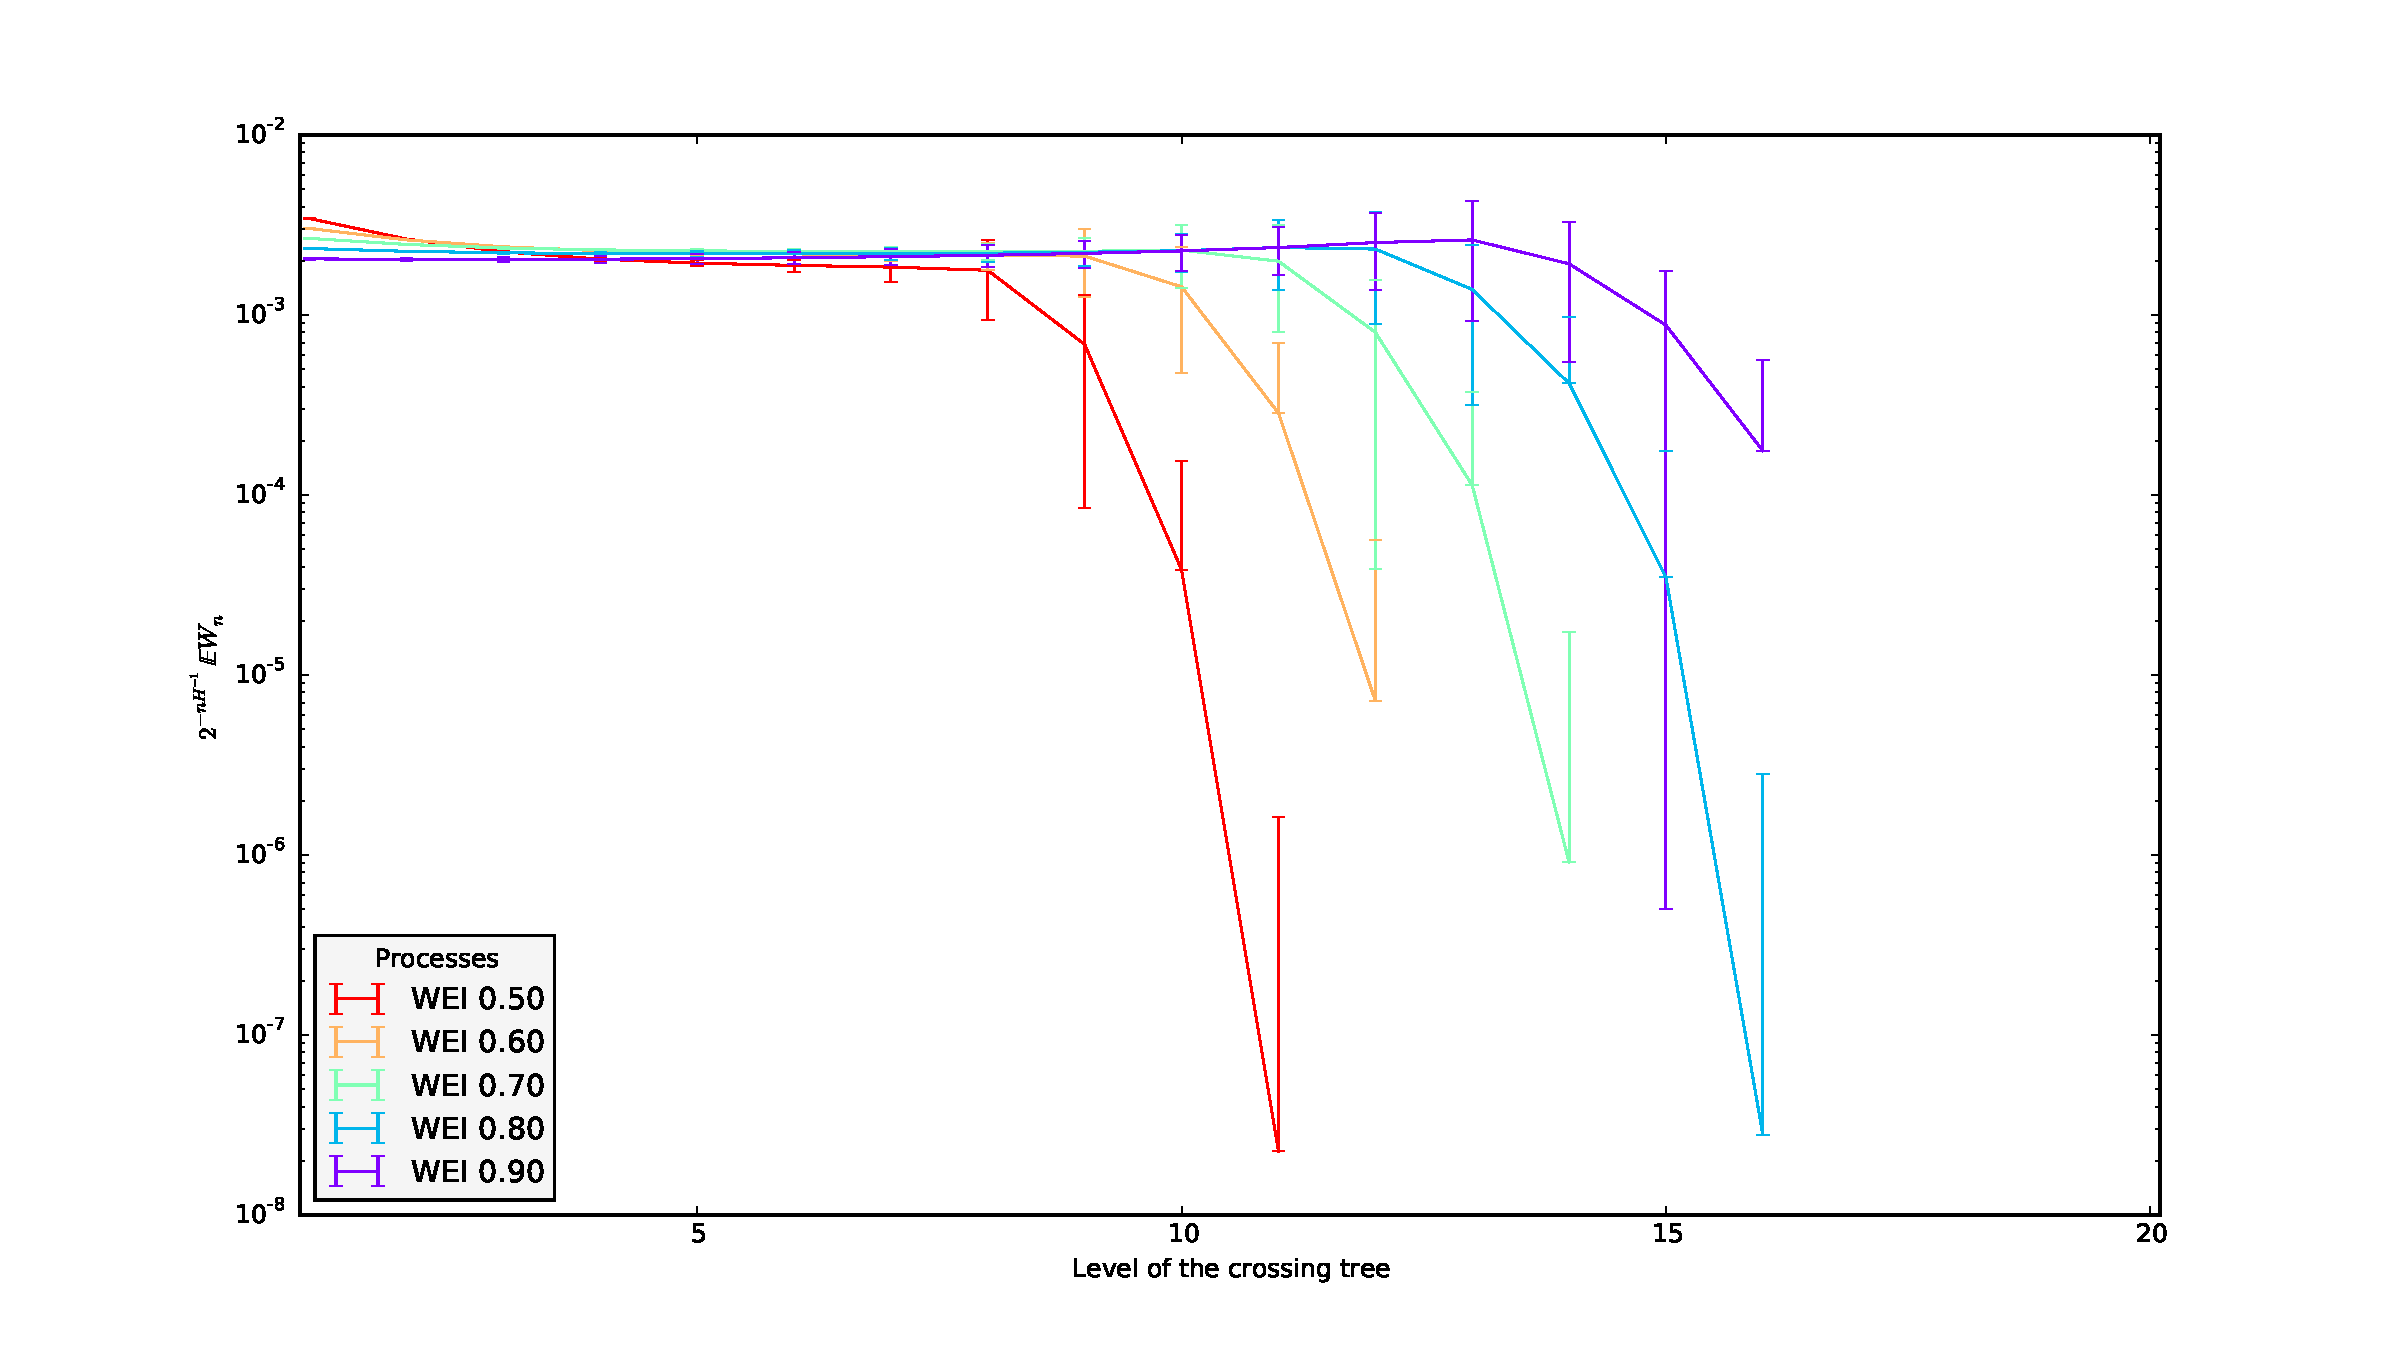
\includegraphics[draft,width=6in]{images/fig_08_med_WEI_10000-17}
    \caption{The average crossing duration at each level of the crossing tree built
    for the Weierstrass processes.}
\label{fig:wei_durations}
\end{center}\end{figure}

\begin{figure}[htb]\begin{center}
    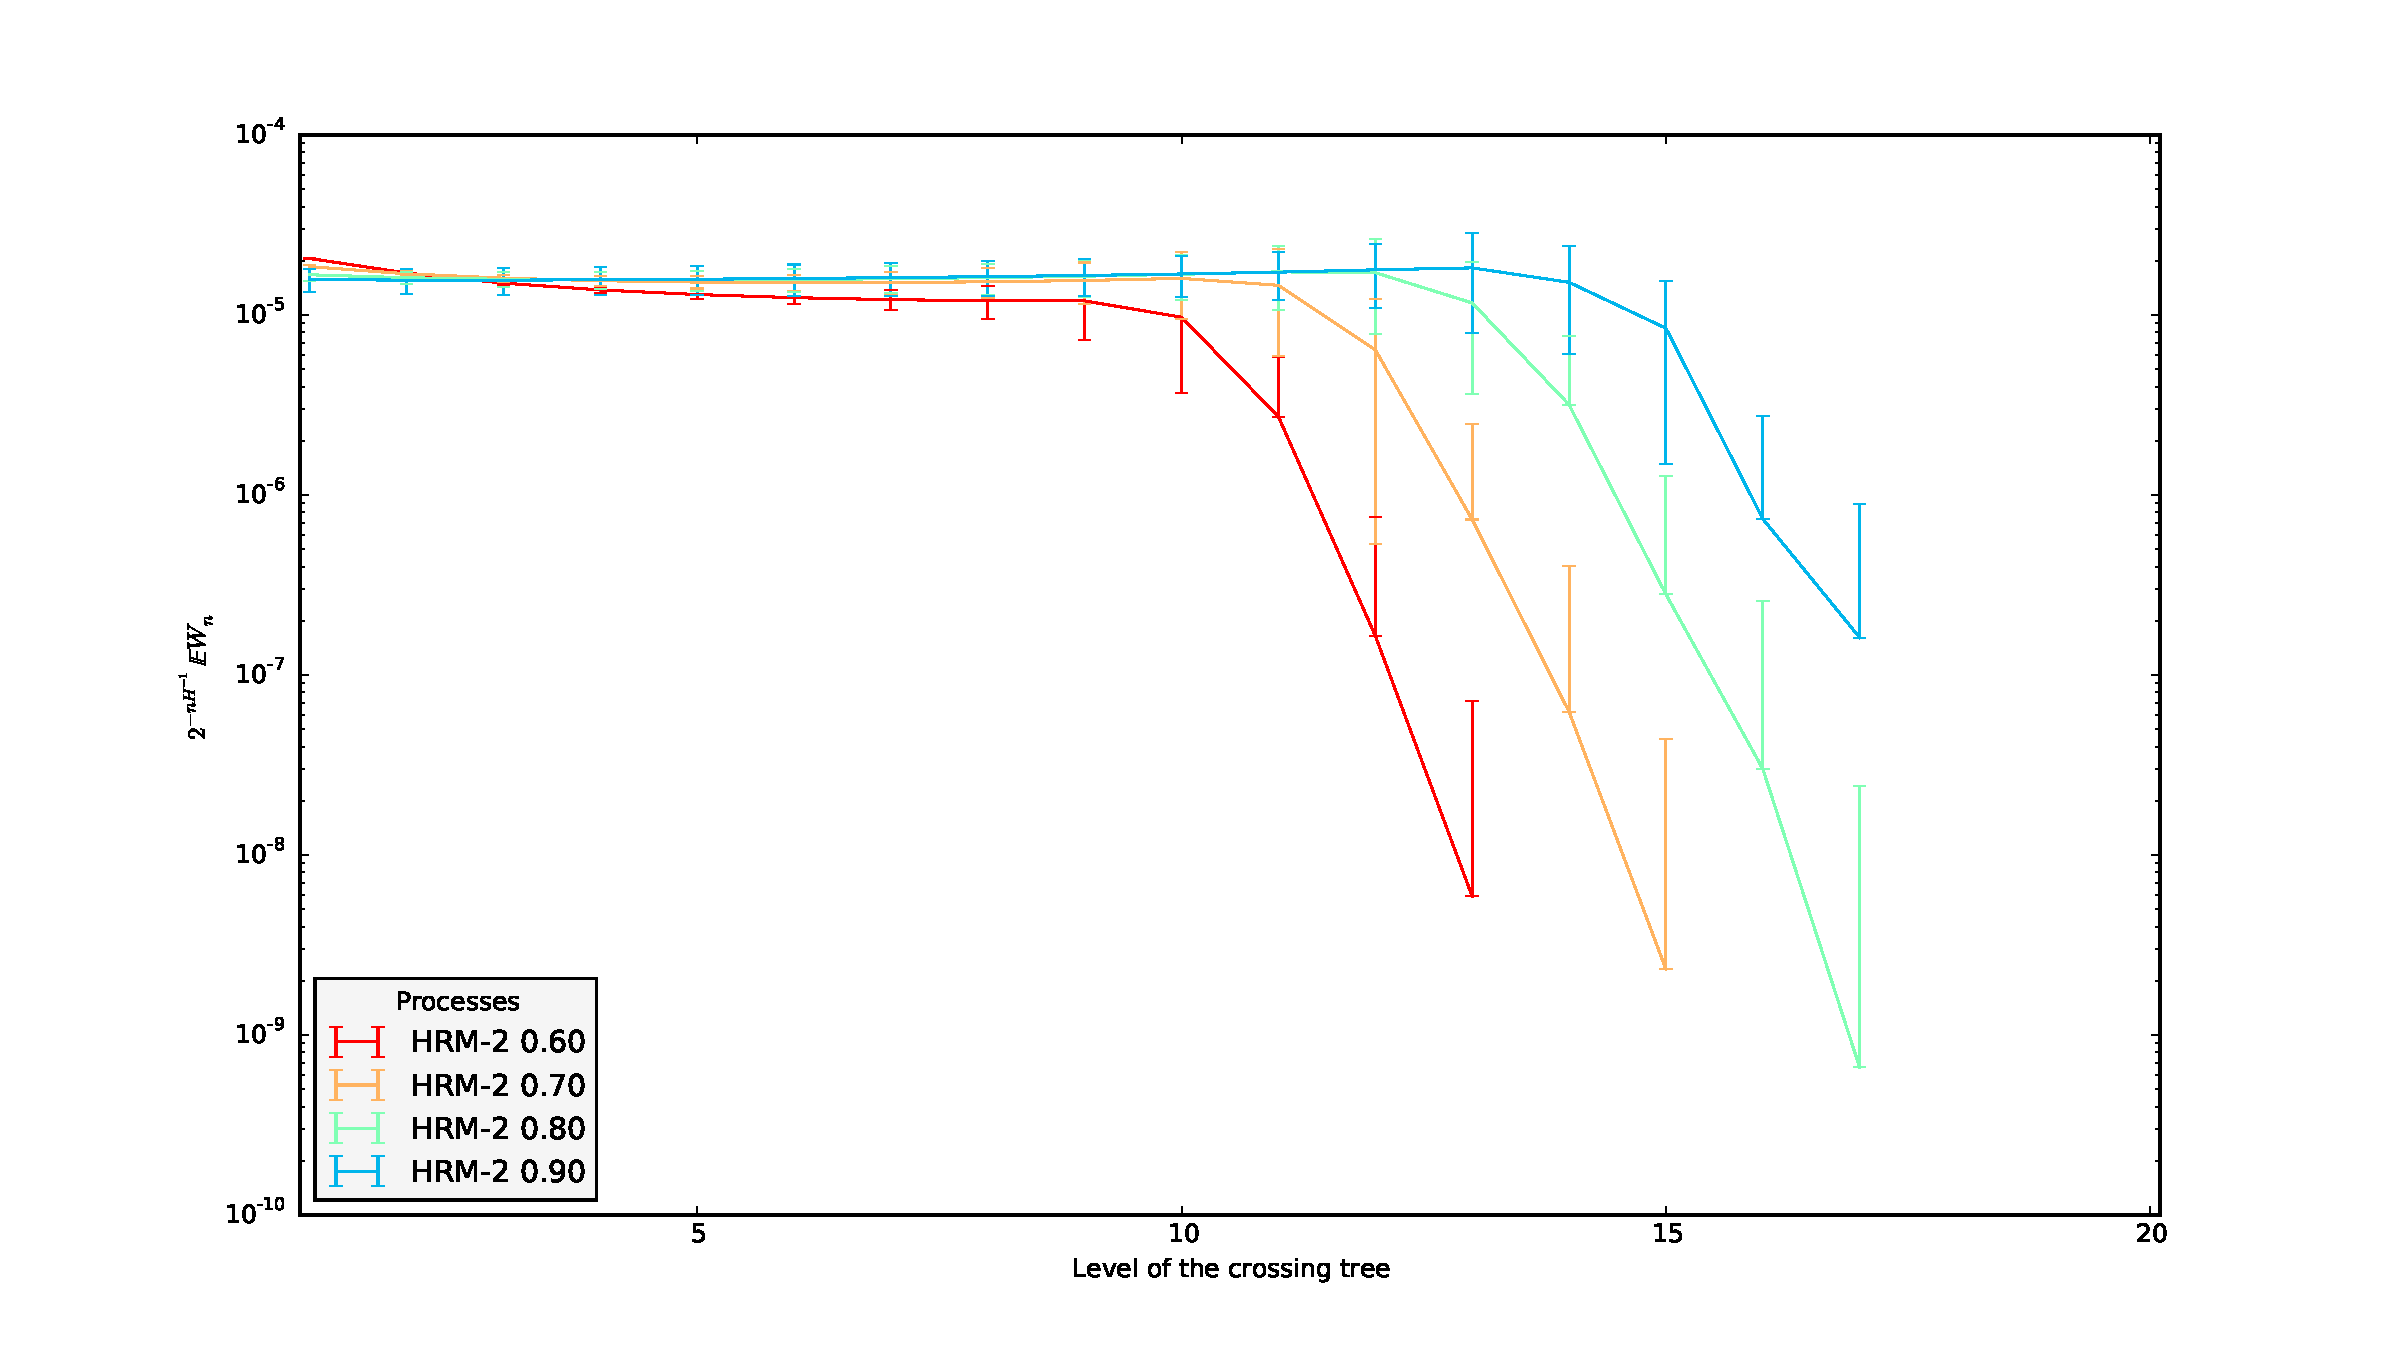
\includegraphics[draft,width=6in]{images/fig_08_med_HRM-2_10000-17}
    \caption{The average crossing duration at each level of the crossing tree built
    for the Hermite processes of order $2$.}
\label{fig:hrm_2_durations}
\end{center}\end{figure}

\begin{figure}[htb]\begin{center}
    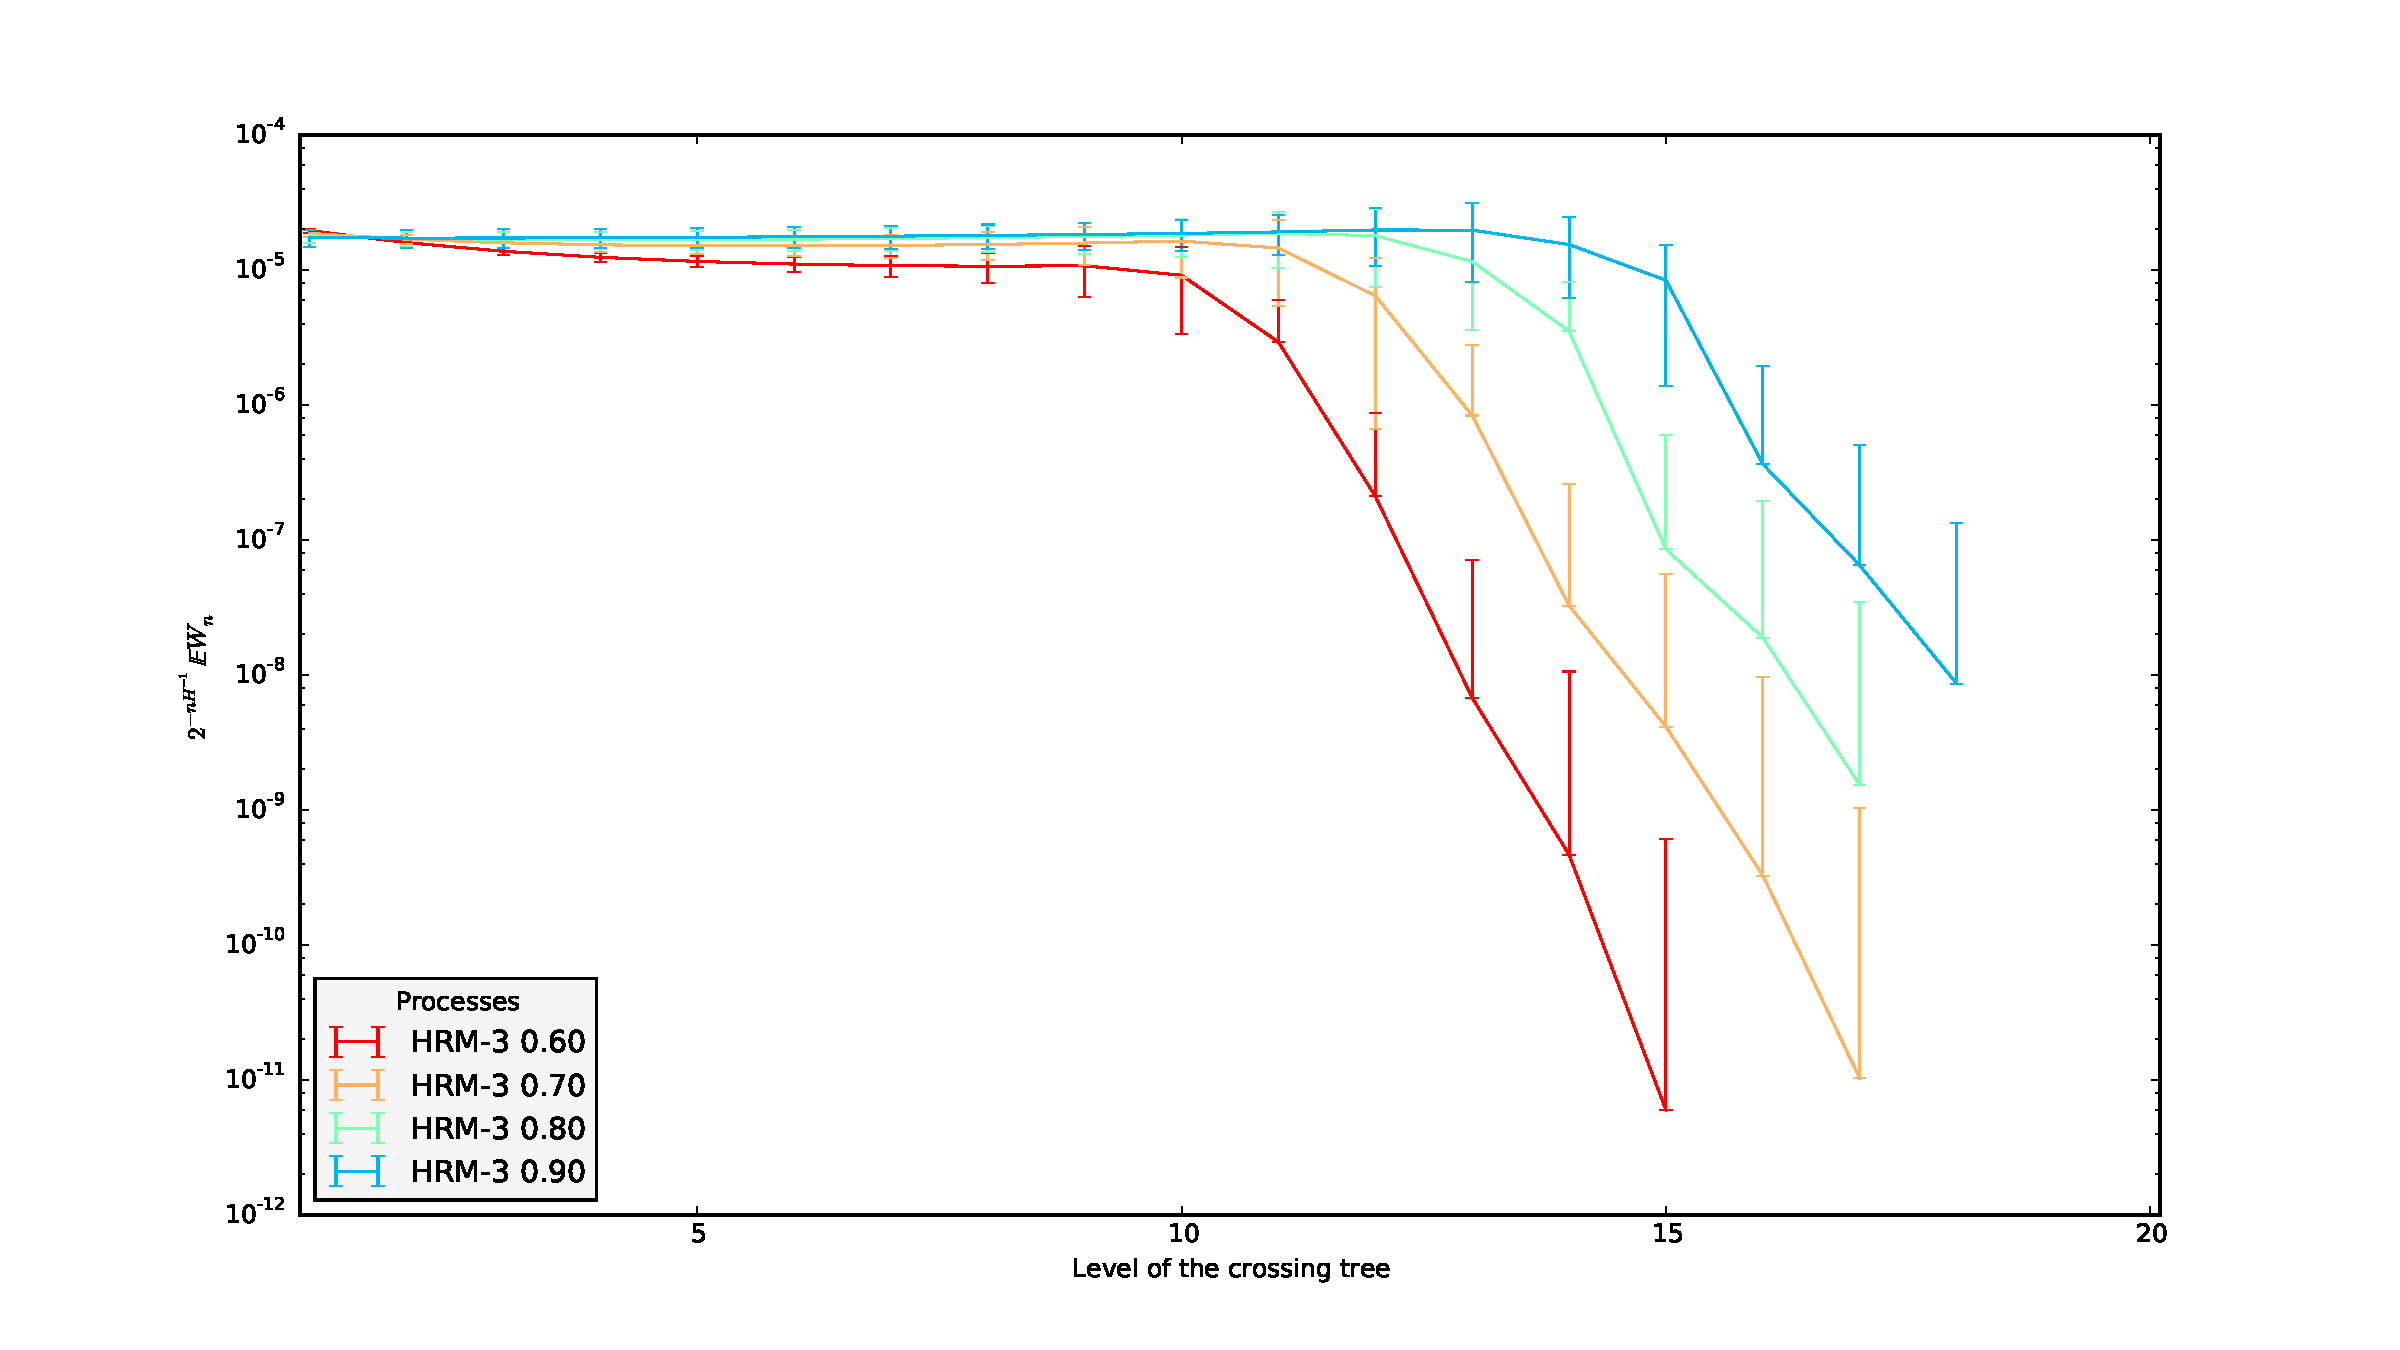
\includegraphics[draft,width=6in]{images/fig_08_med_HRM-3_10000-17}
    \caption{The average crossing duration at each level of the crossing tree built
    for the Hermite processes of order $3$.}
\label{fig:hrm_3_durations}
\end{center}\end{figure}

\begin{figure}[htb]\begin{center}
    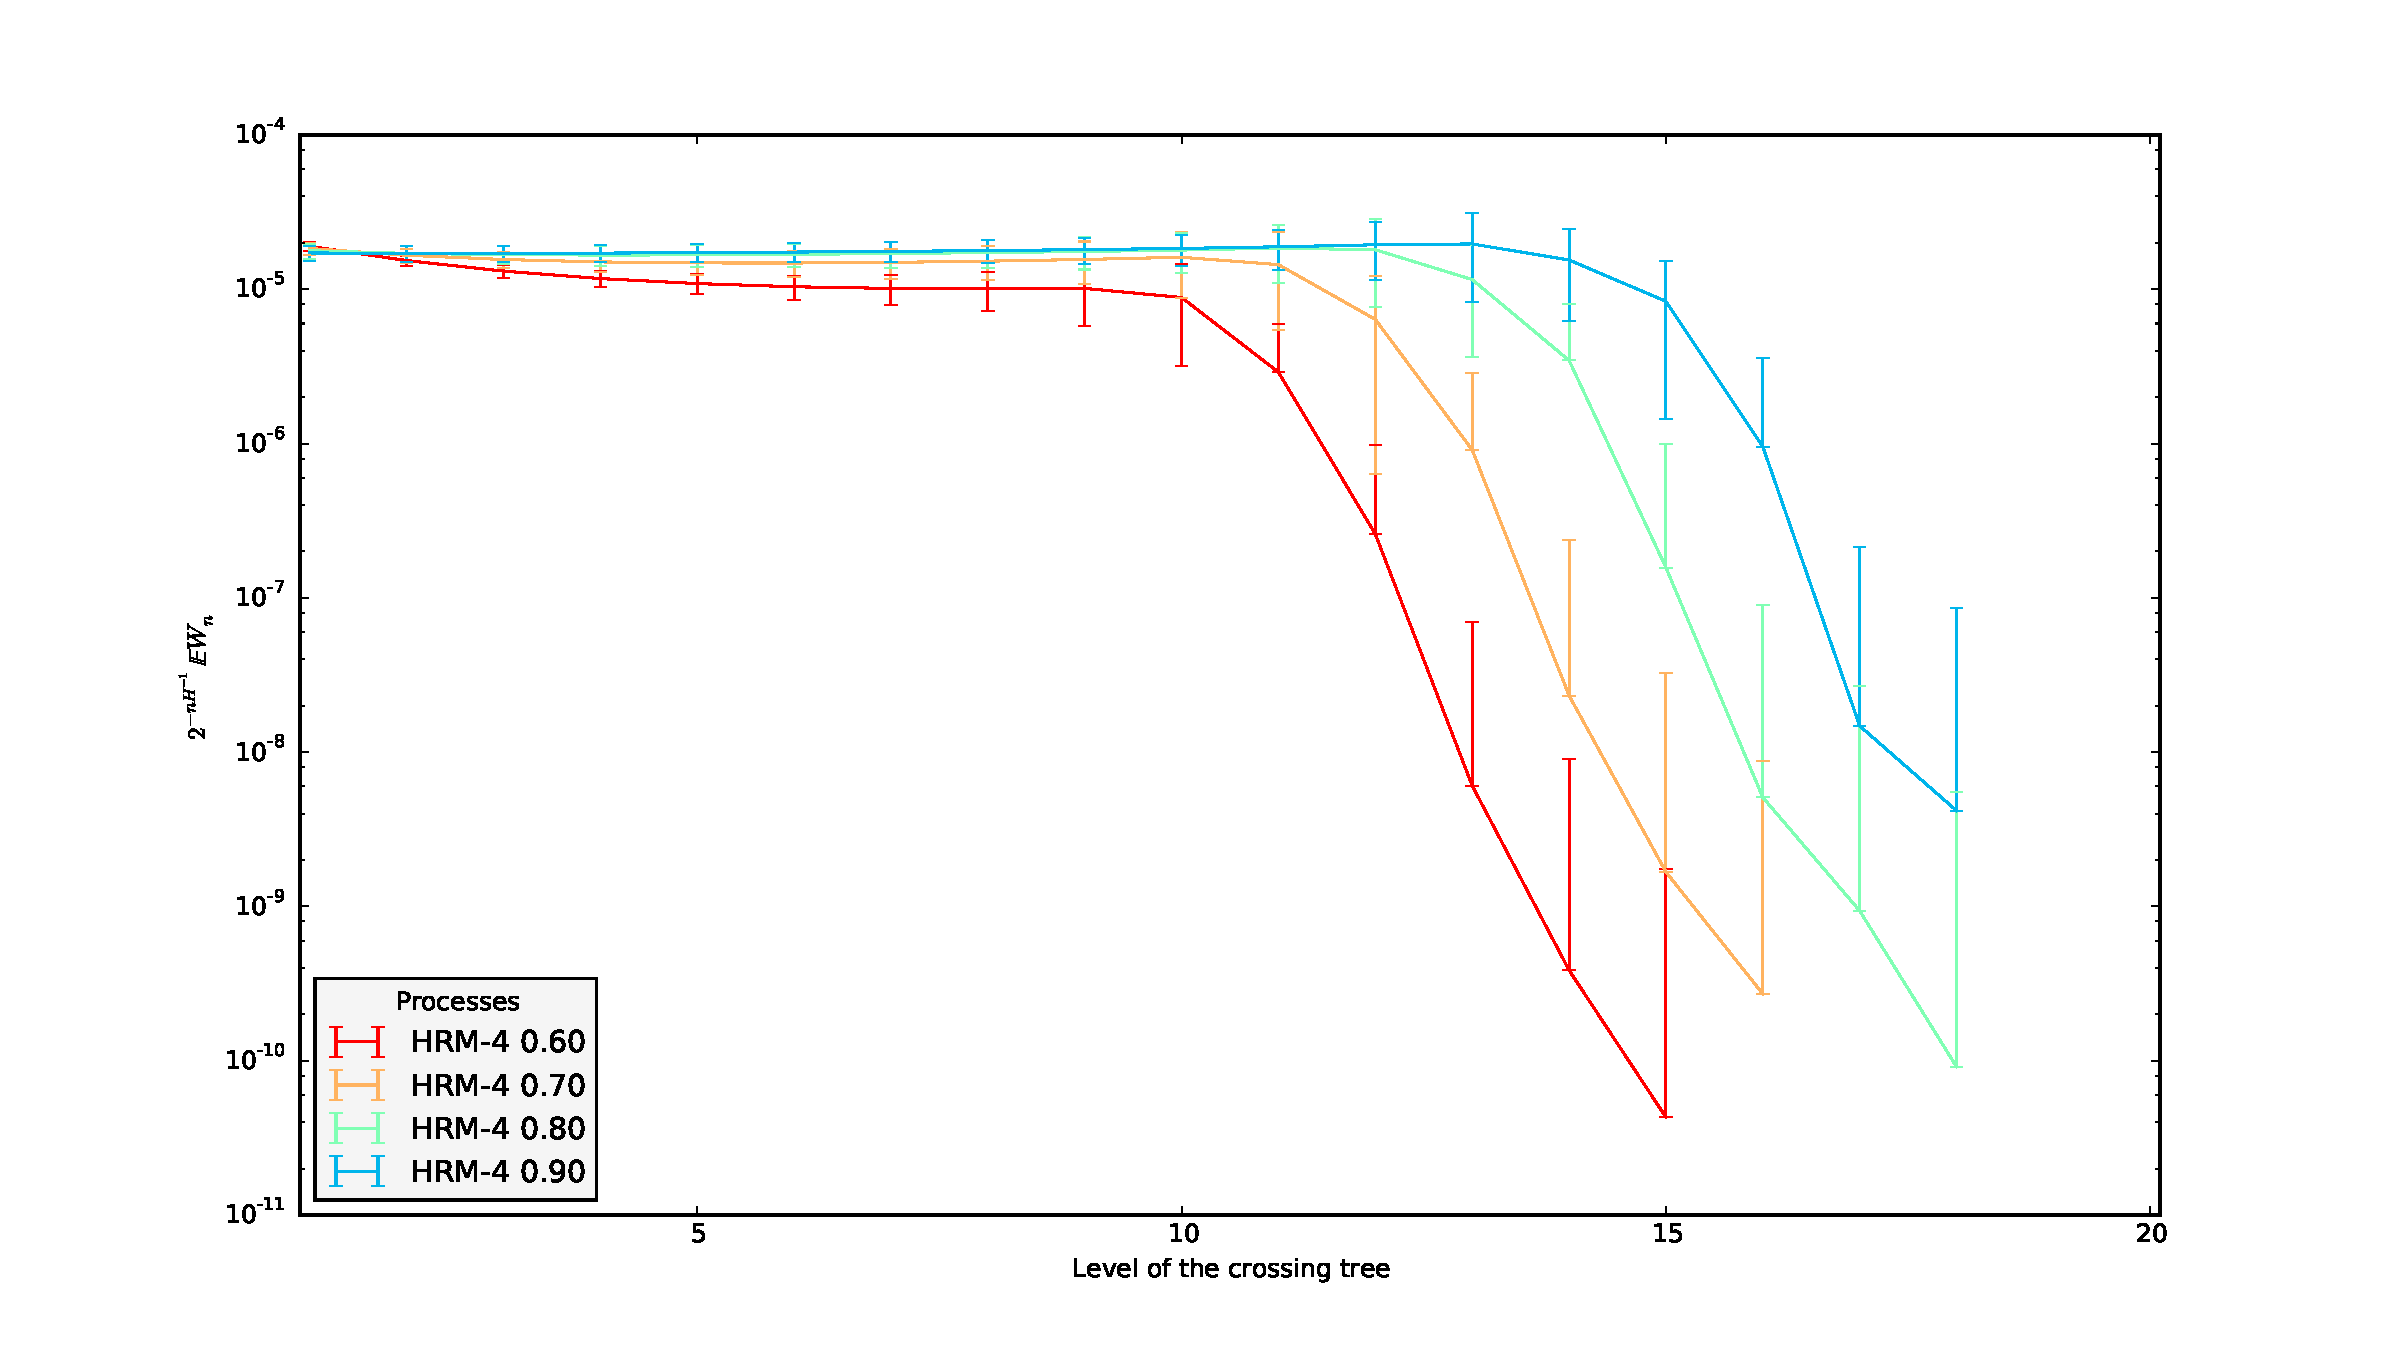
\includegraphics[draft,width=6in]{images/fig_08_med_HRM-4_10000-17}
    \caption{The average crossing duration at each level of the crossing tree built
    for the Hermite processes of order $4$.}
\label{fig:hrm_4_durations}
\end{center}\end{figure}

\begin{figure}[htb]\begin{center}
    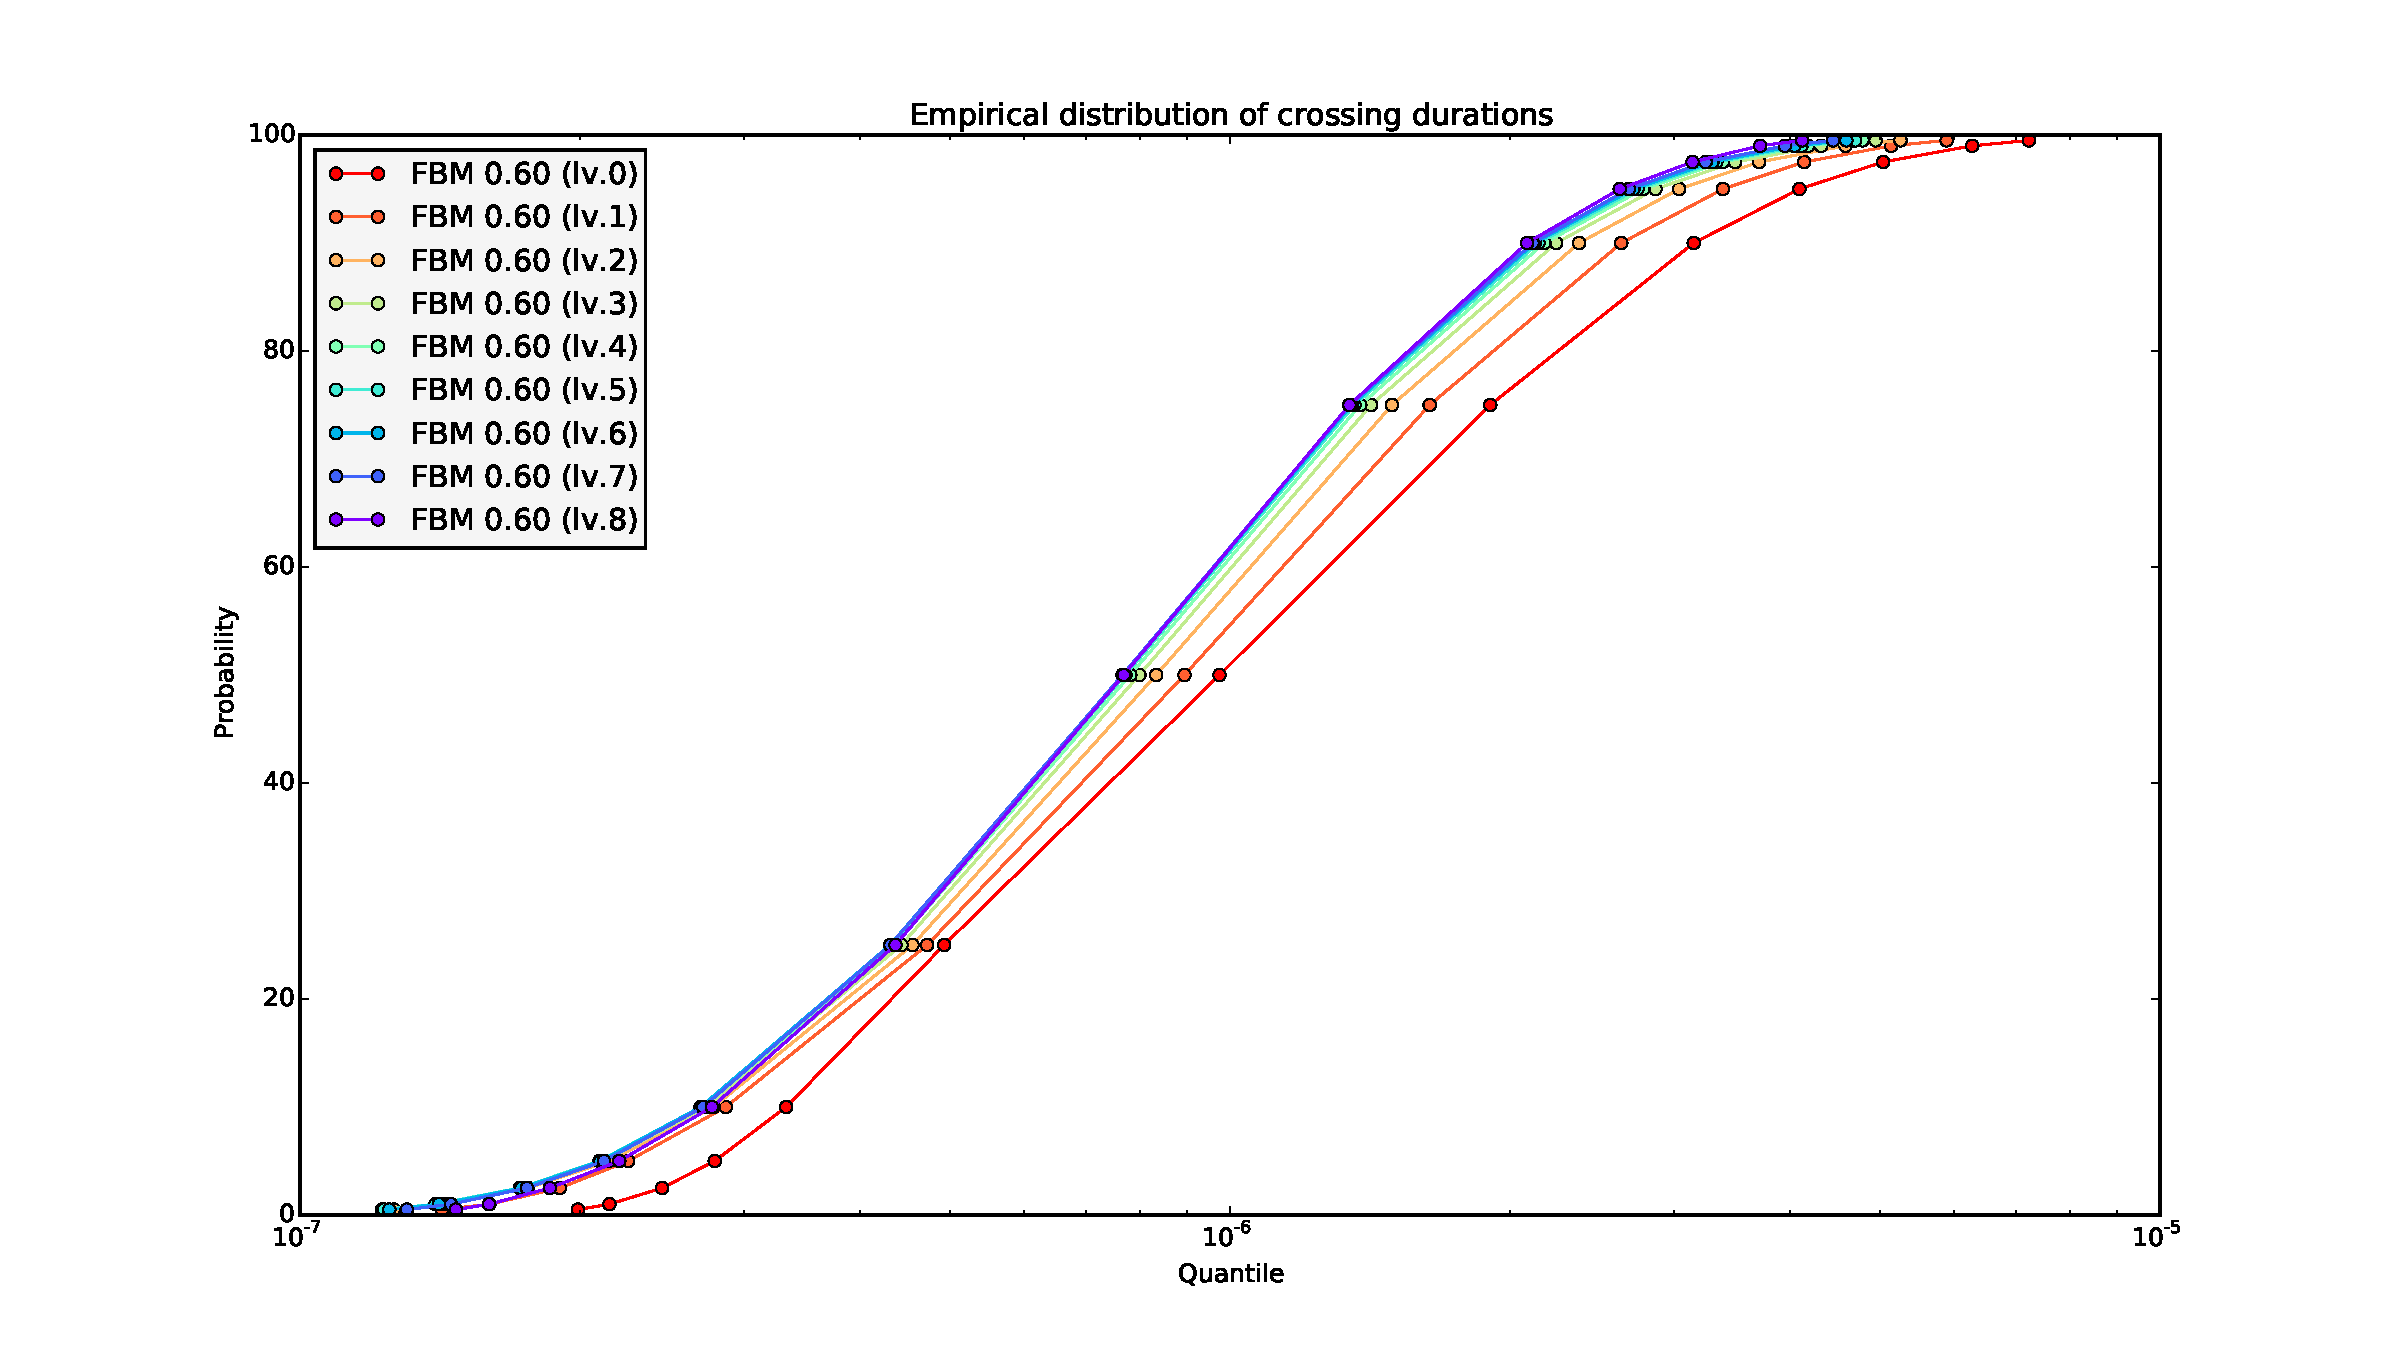
\includegraphics[draft,width=6in]{images/fig_09_med_FBM_060}
    \caption{The empirical distribution of crossing durations at each level of the
    crossing tree built for the fractional Brownian motion ($2^{21}$ datapoints) with $H = 0.6$.
    Averaged across all Monte-Carlo realisations.}
\label{fig:fbm_quantiles_06}
\end{center}\end{figure}

\begin{figure}[htb]\begin{center}
    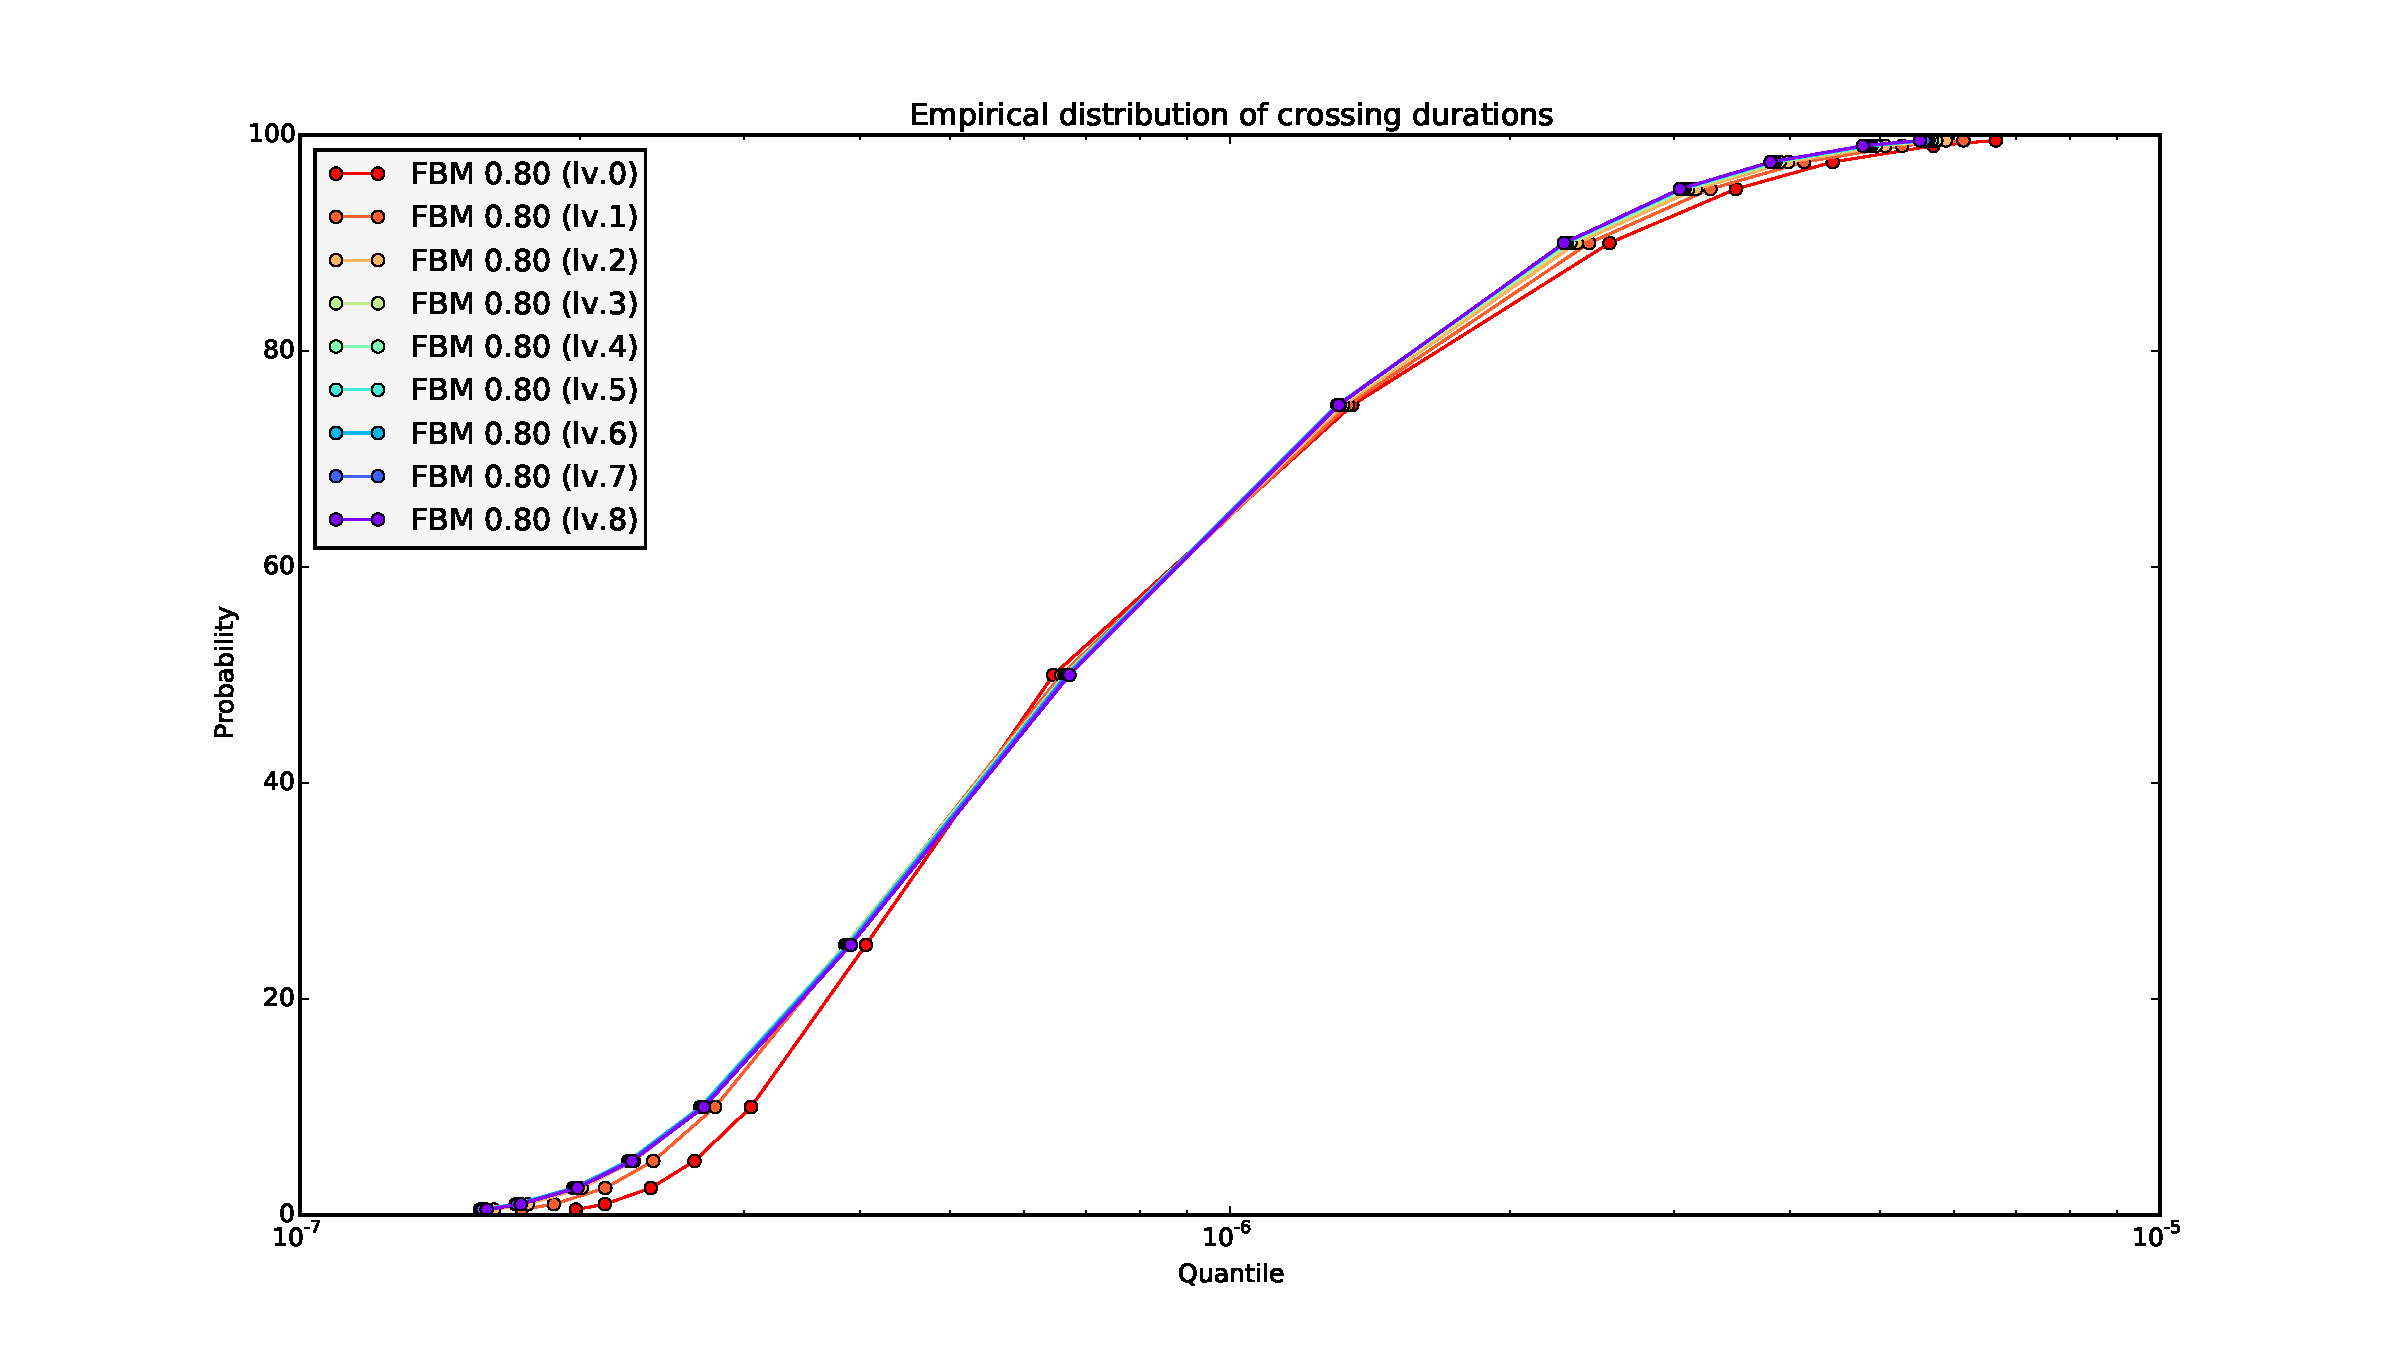
\includegraphics[draft,width=6in]{images/fig_09_med_FBM_080}
    \caption{Similarly to figure~\ref{fig:fbm_quantiles_06} but for fBM with $H=0.8$.}
\label{fig:fbm_quantiles_08}
\end{center}\end{figure}

\begin{figure}[htb]\begin{center}
    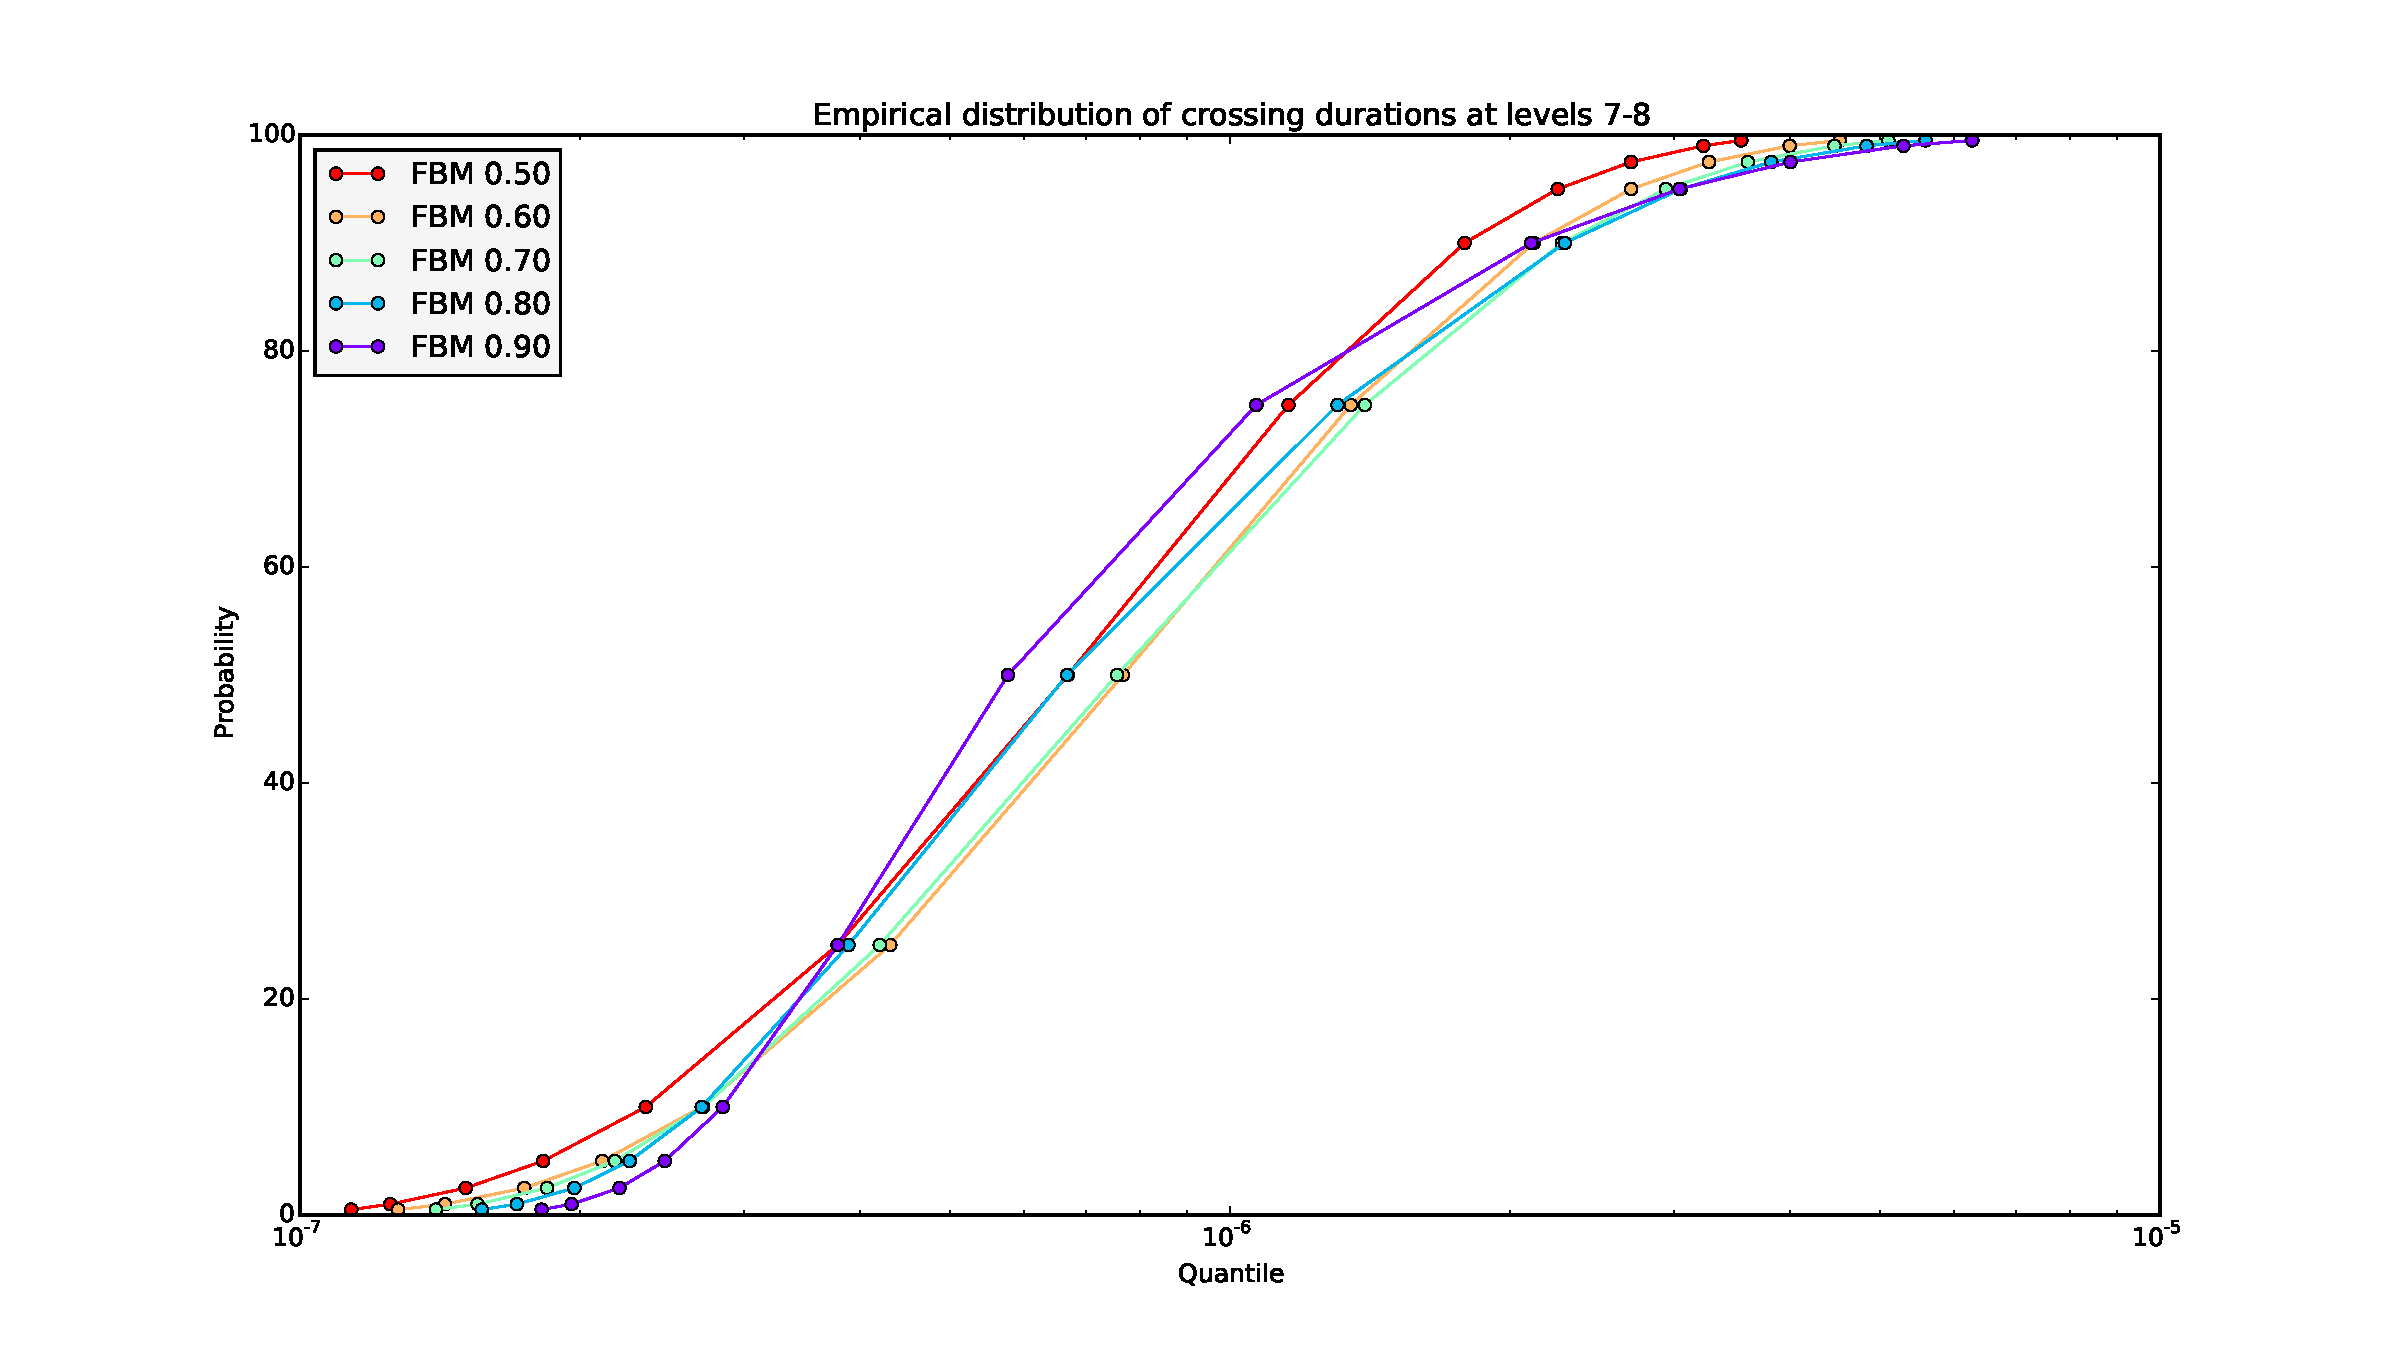
\includegraphics[draft,width=6in]{images/fig_10_med_FBM}
    \caption{Empirical distributions of crossing durations estimated on levels 7-8
    for the fBM ($2^{21}$ datapoints). Averaged across all Monte-Carlo realisations.}
\label{fig:fbm_quantiles_durations}
\end{center}\end{figure}

% subsection results (end)

% section experiment (end)

\section{Conclusion and further work} % (fold)
\label{sec:conlusion_and_further_work}

This preformed extensive Monte-Carlo simulation suggests, that the considered
classes of $H$-SSSI stochastic processes indeed shares common statistical properties
of the crossing tree. To findings are summarized below: \begin{enumerate}
	\item The crossing tree seems capable of correctly identifying the Hurst
	exponent of the studied series, provided correct tree levels are chosen to
	produce the estimate. The tree levels should not be too close to the leaves
	of the tree, for the sake of avoiding excessive bias due to linear interpolation,
	and be such that there is no statistical evidence to significant variations
	in the offspring distribution at each level;
	\item Processes seem to share similar shape of the empirical distribution of
	the crossing sizes (the number of offspring), though the hypothesized
	relationship between the offspring distribution and the Hurst exponent
	does not seem to hold exactly, (see figures \ref{fig:fbm_offspring_distribution}
	and \ref{fig:all_xing_probs});
	\item The conditional distributions of excursion within each crossing seems
	to agree with the hypothesised values of $2^{\frac{-1}{2H}}$.
	\item The collected empirical evidence seems to confirm similarity of the scaling
	properties of crossing durations across all studied processe.
\end{enumerate}
To summarize, the overall evidence is in favour of the conjecture, it is absolutely
necessary to address the issue of the upward bias in the empirical probabilities of
crossings of size higher than 2.

One of the way in which this study can be improved is the generation of samples paths
of Hermite stochastic processes. Another line of inquiry in the topic of crossing trees
if their application to machine learning and generalization to higher dimensions, which
would find application in image processing. The third possible extension is the utilization
of the crossing tree, or its modification, in the problem of early detection of structural
breaks in univariate or multivariate time series data.

% section conlusion_and_further_work (end)

\bibliographystyle{IEEEbib}
\bibliography{literature}
\end{document}
